\section{Estimation of QCD in the $l\tau$ and $l\rm{jet}$ channel}


\begin{figure}
    \centering
    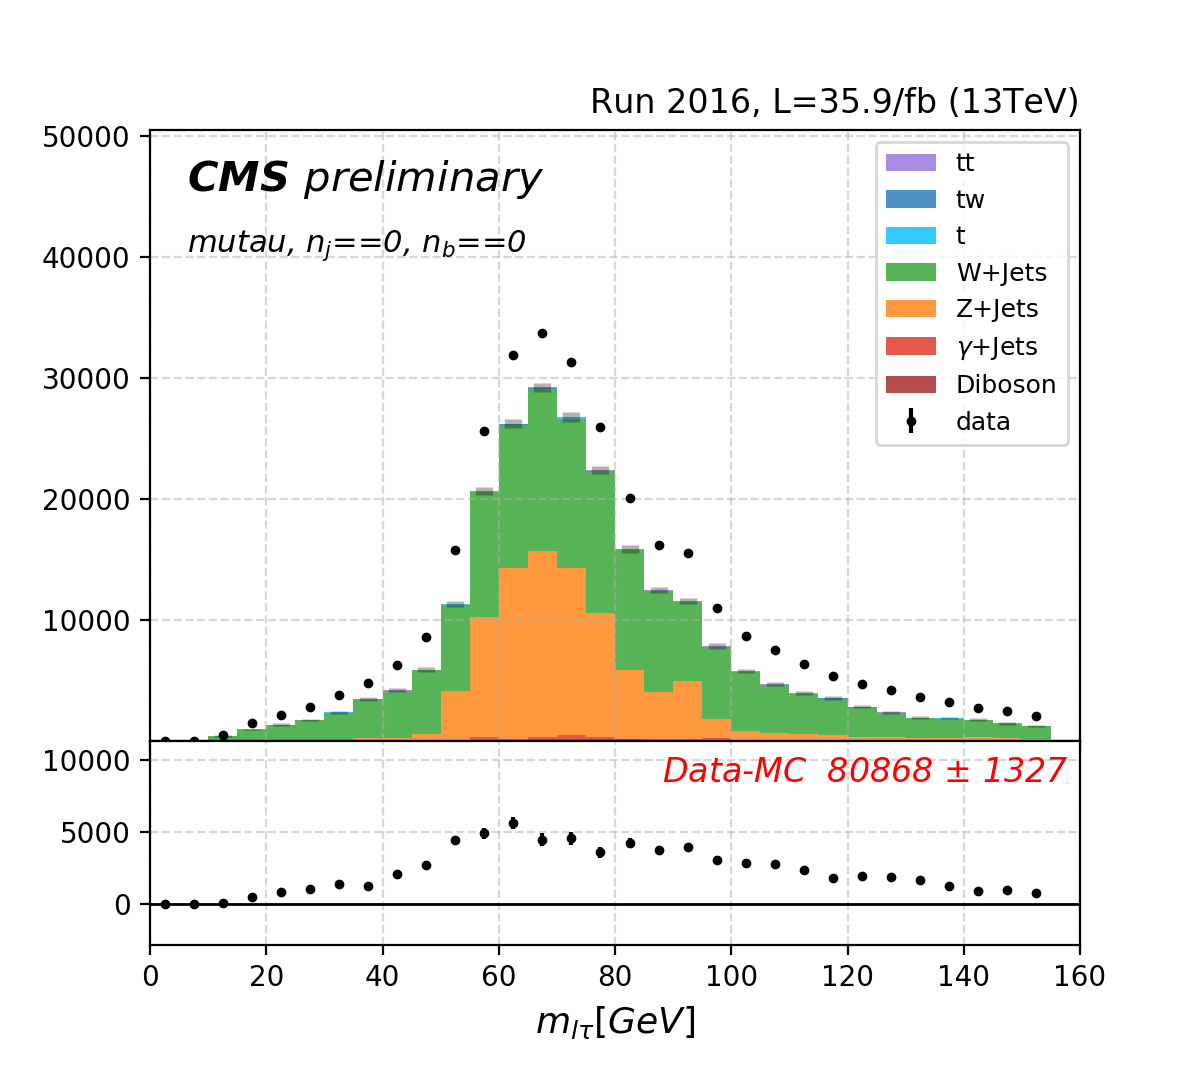
\includegraphics[width=0.24\textwidth]{chapters/Appendix/sectionQCD/figures/mutau_==0_==0_dilepton_mass.png}
    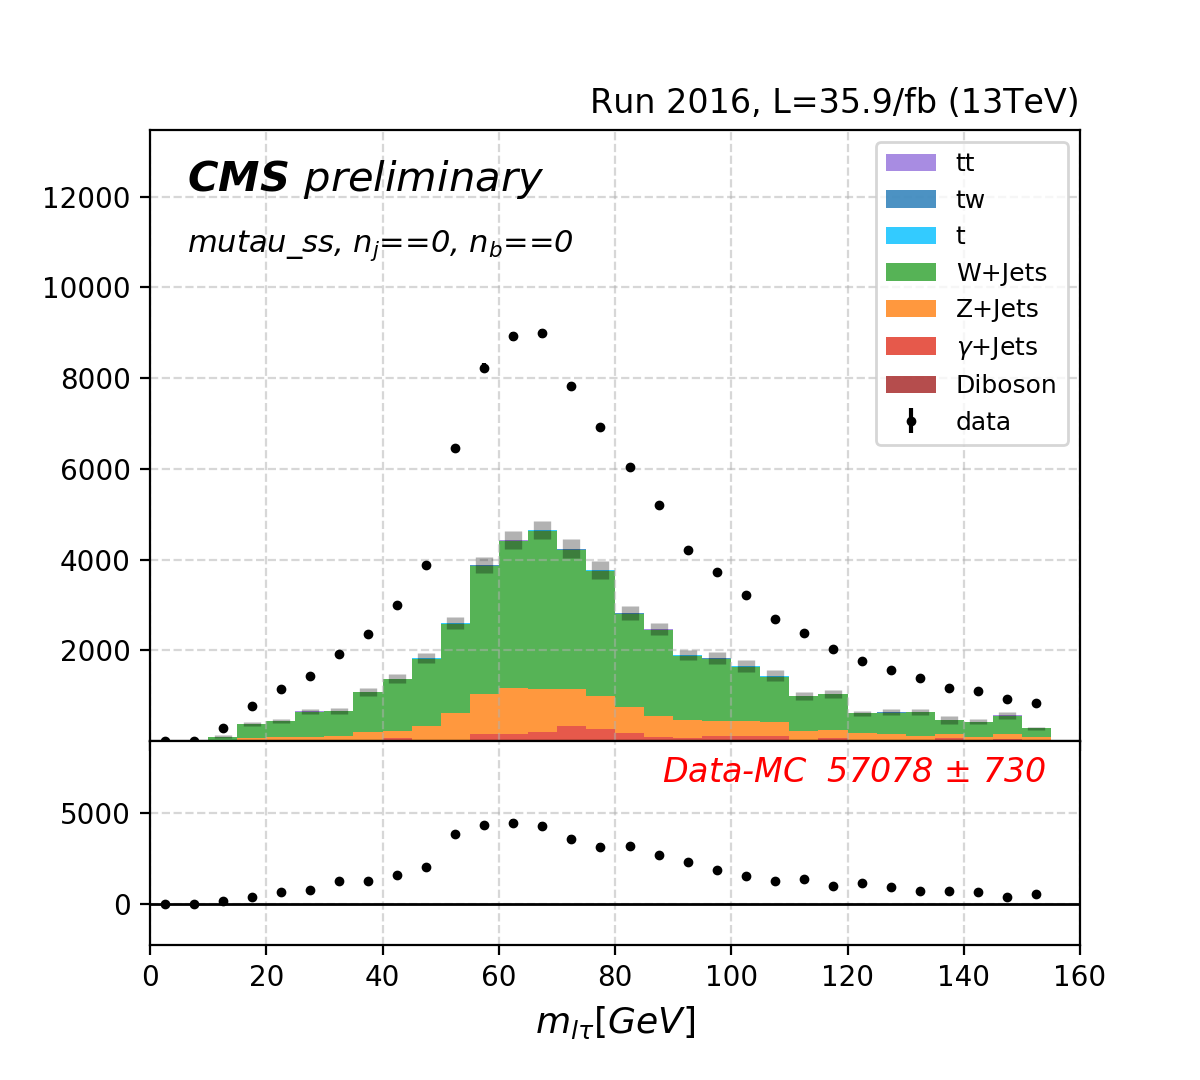
\includegraphics[width=0.24\textwidth]{chapters/Appendix/sectionQCD/figures/mutau_ss_==0_==0_dilepton_mass.png}
    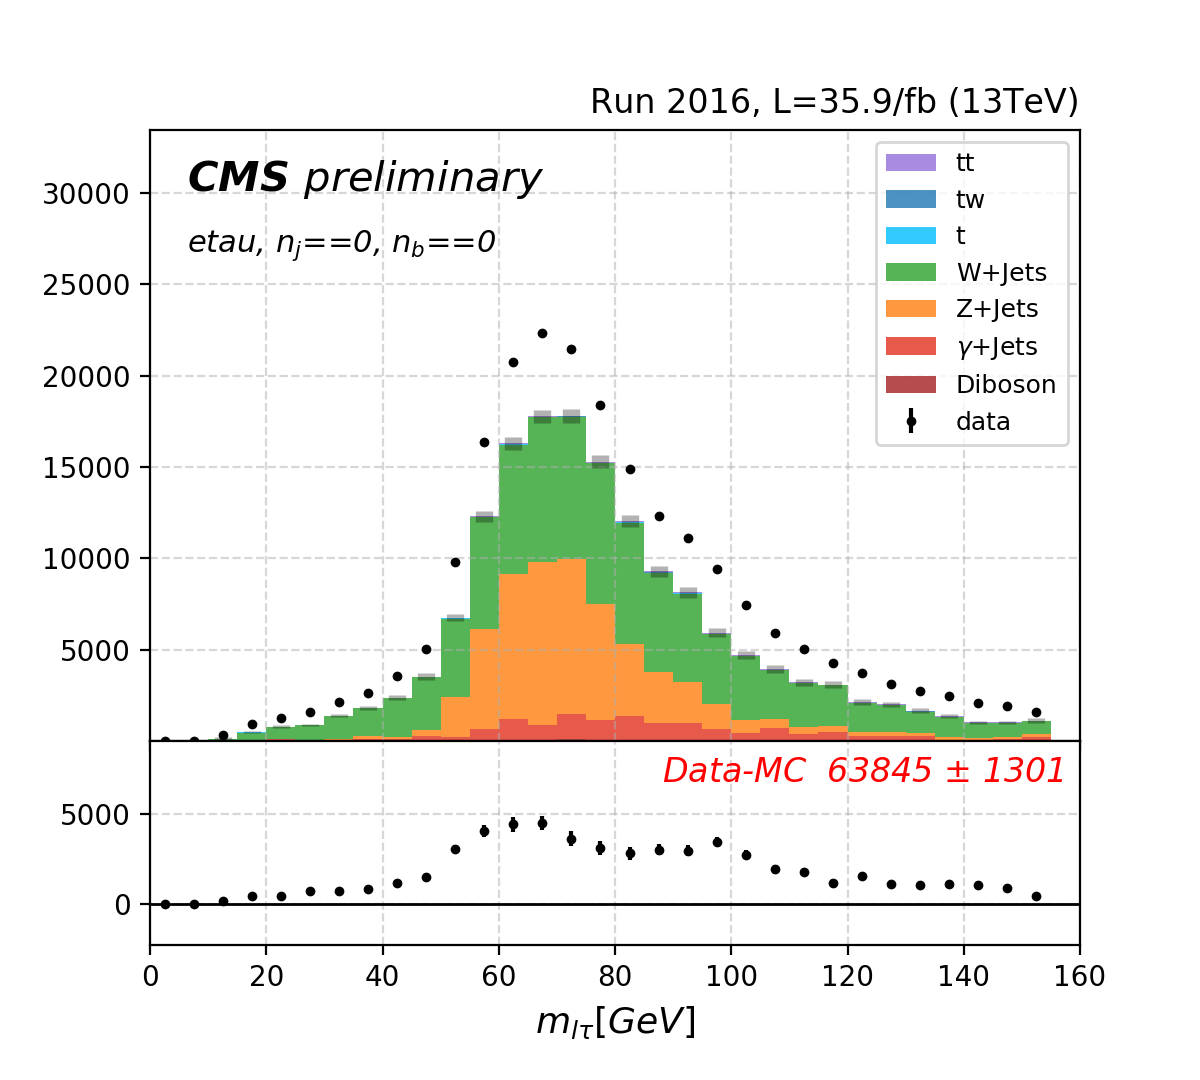
\includegraphics[width=0.24\textwidth]{chapters/Appendix/sectionQCD/figures/etau_==0_==0_dilepton_mass.png}
    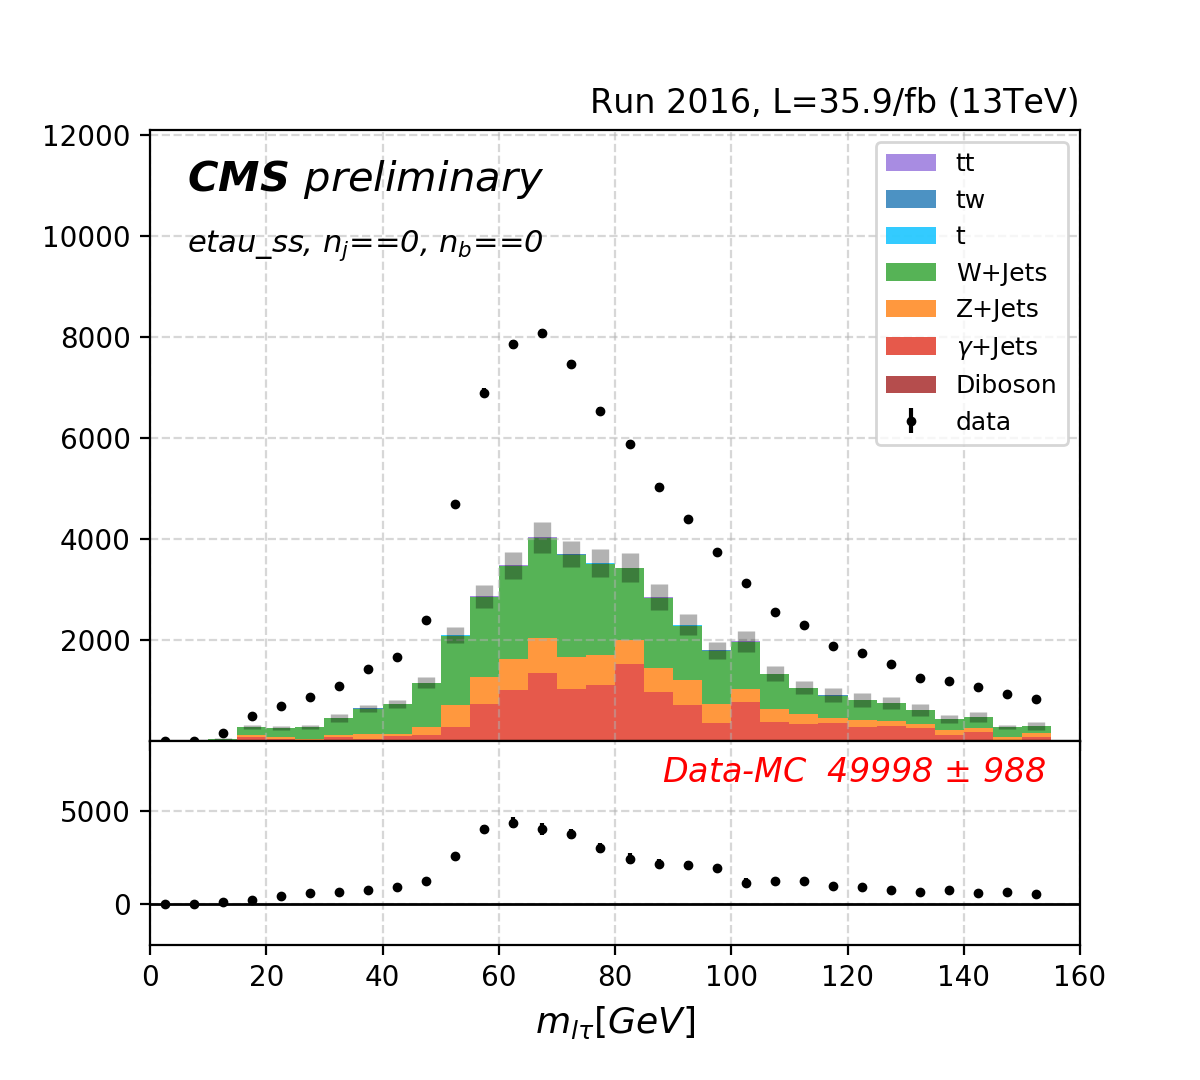
\includegraphics[width=0.24\textwidth]{chapters/Appendix/sectionQCD/figures/etau_ss_==0_==0_dilepton_mass.png}
    
    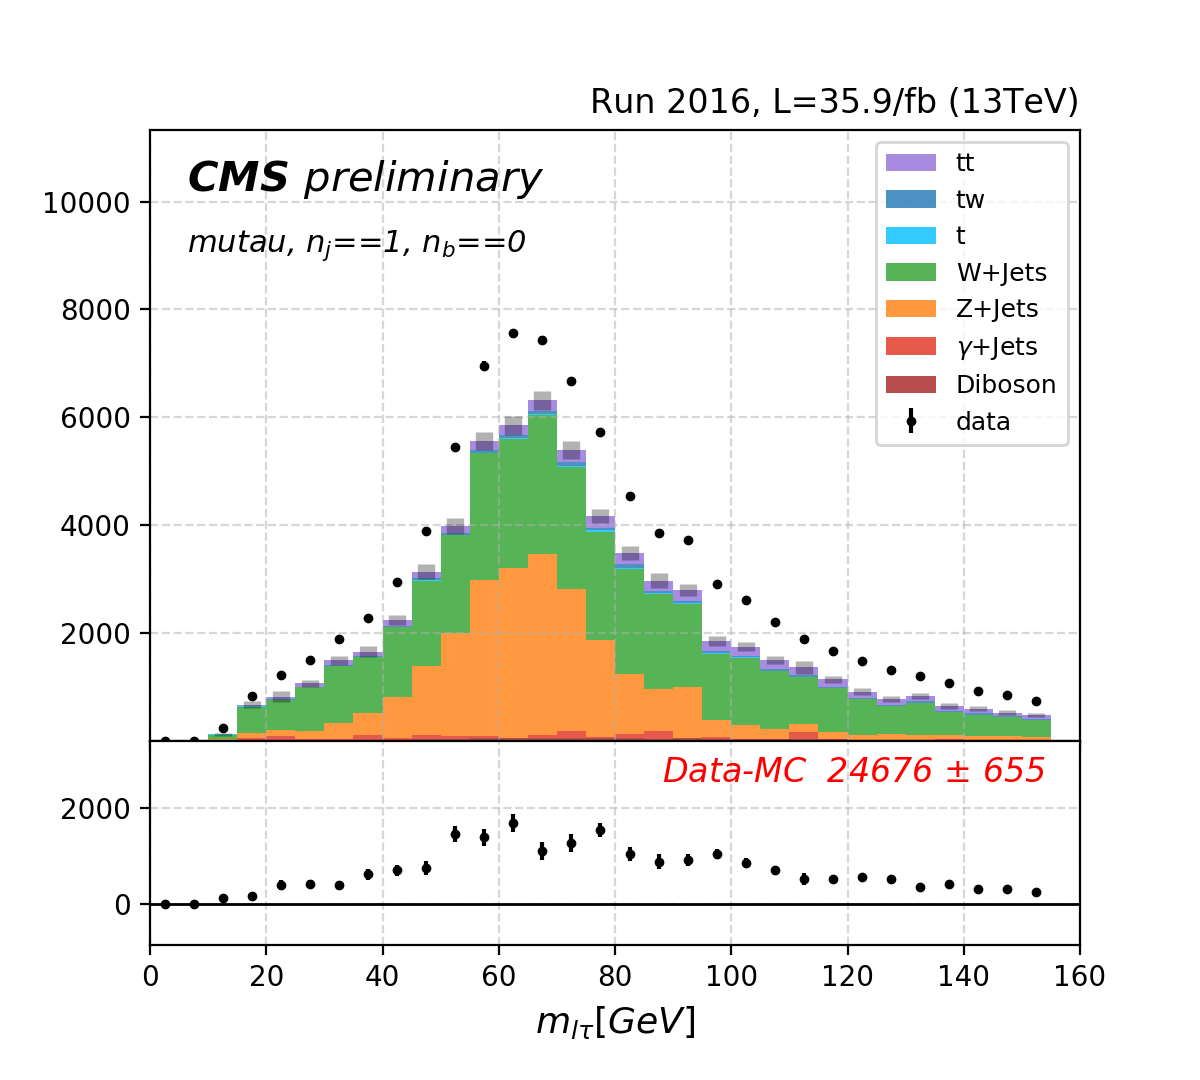
\includegraphics[width=0.24\textwidth]{chapters/Appendix/sectionQCD/figures/mutau_==1_==0_dilepton_mass.png}
    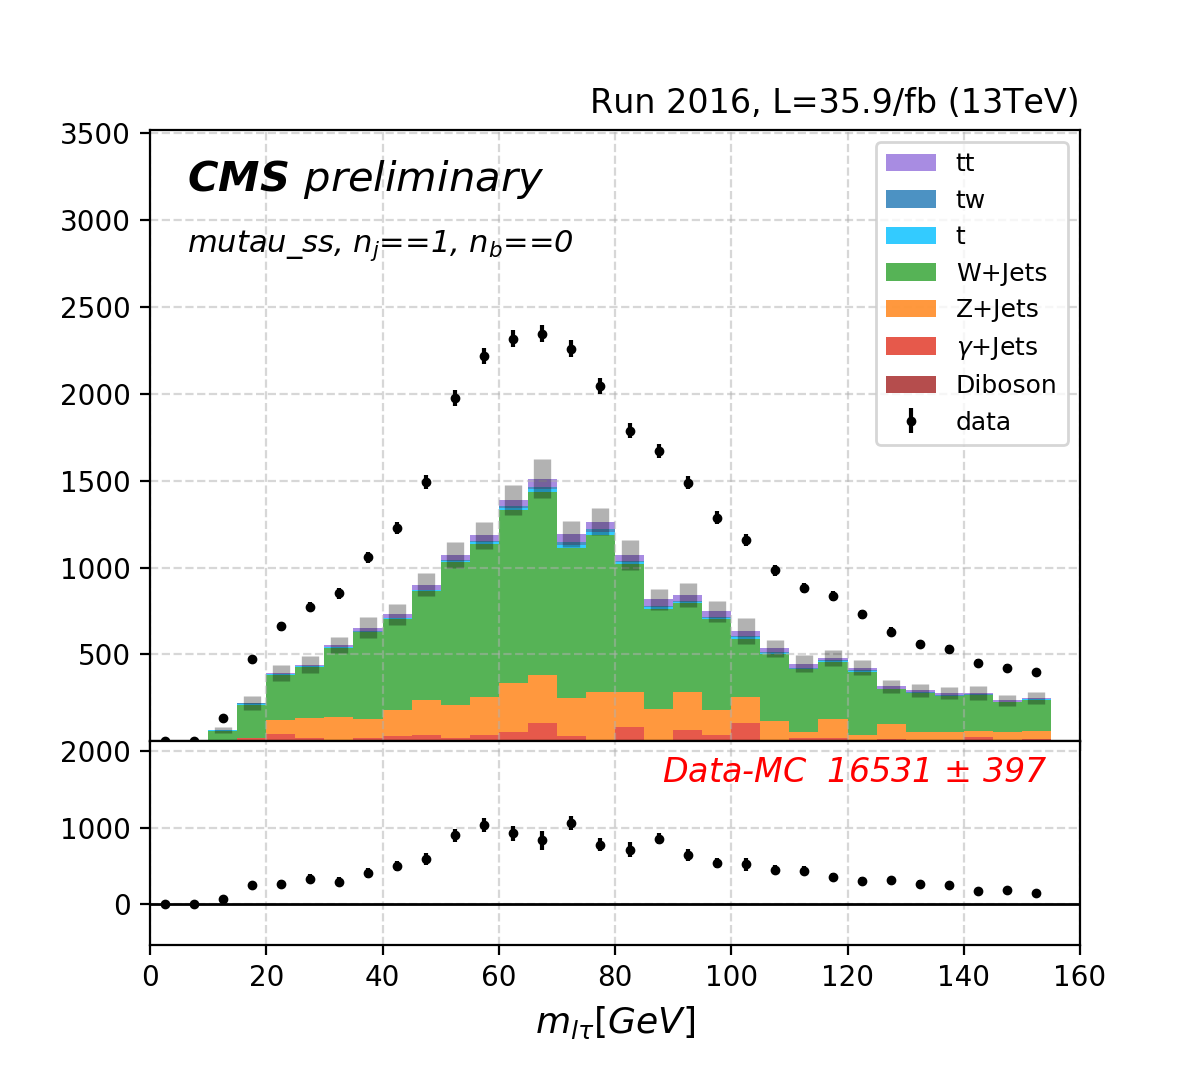
\includegraphics[width=0.24\textwidth]{chapters/Appendix/sectionQCD/figures/mutau_ss_==1_==0_dilepton_mass.png}
    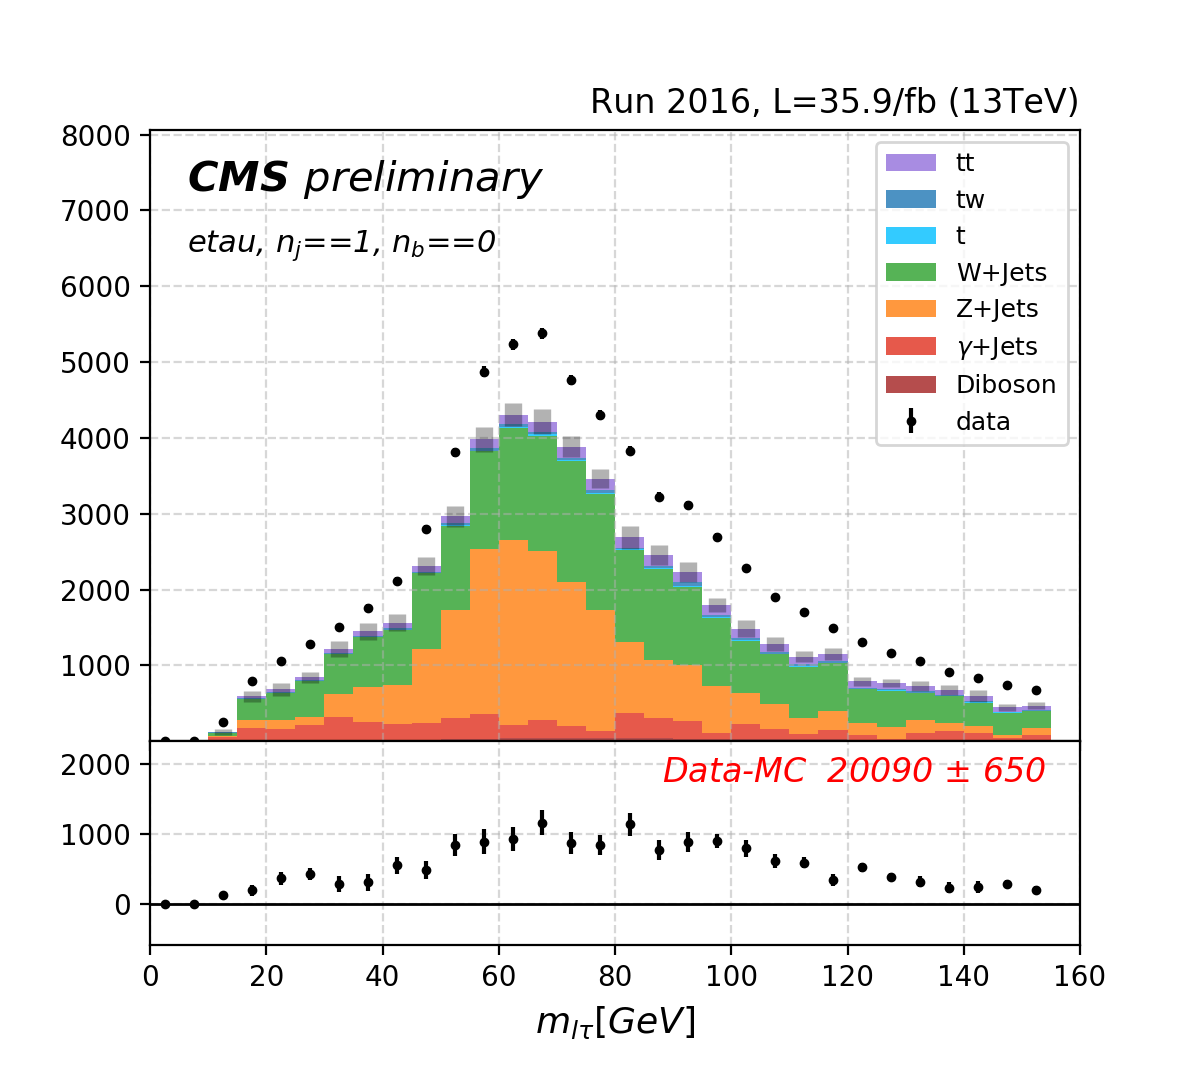
\includegraphics[width=0.24\textwidth]{chapters/Appendix/sectionQCD/figures/etau_==1_==0_dilepton_mass.png}
    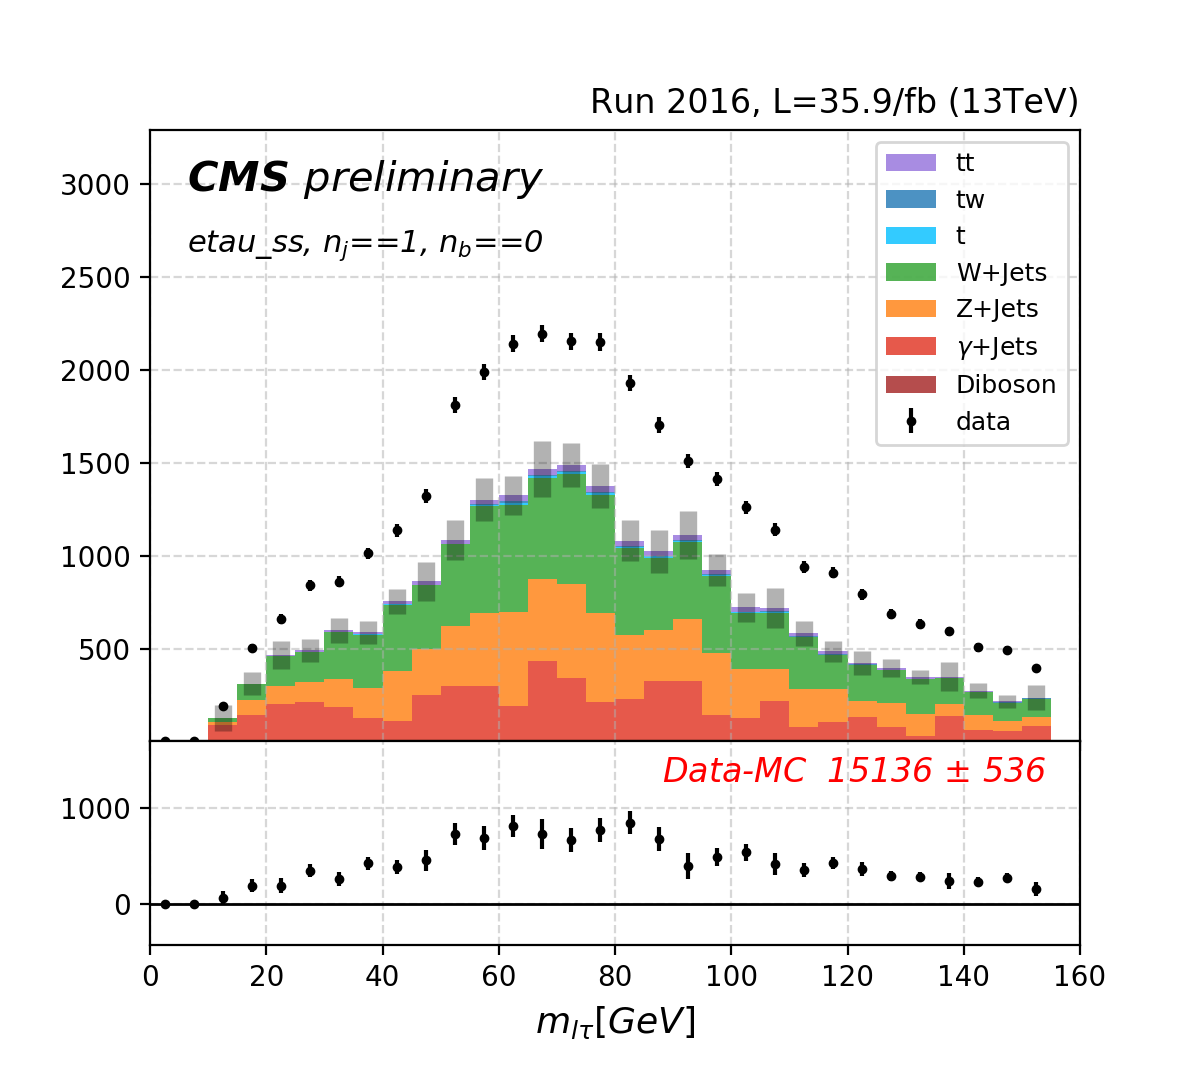
\includegraphics[width=0.24\textwidth]{chapters/Appendix/sectionQCD/figures/etau_ss_==1_==0_dilepton_mass.png}
    
    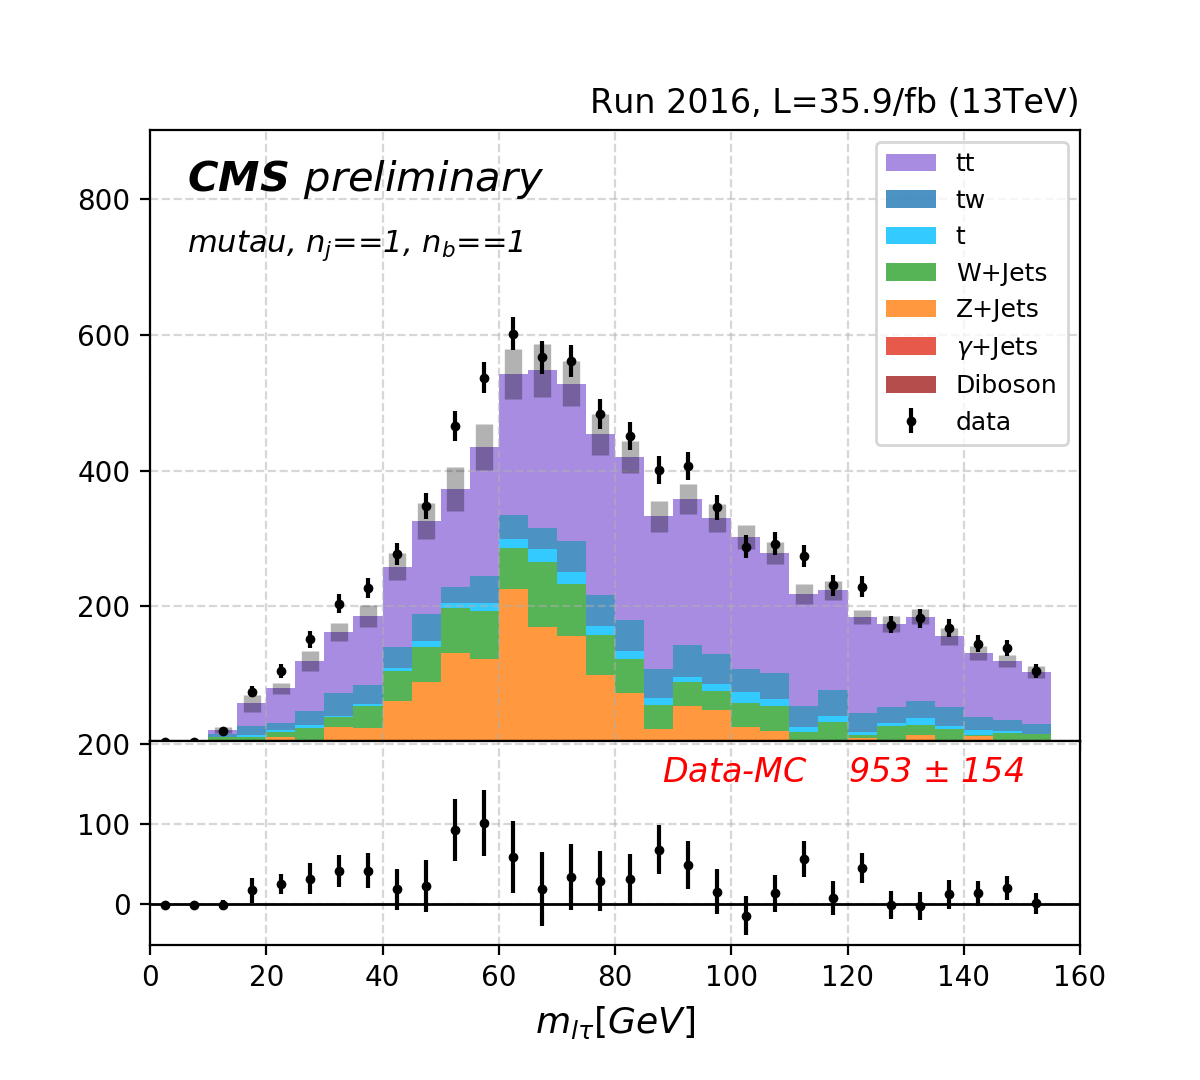
\includegraphics[width=0.24\textwidth]{chapters/Appendix/sectionQCD/figures/mutau_==1_==1_dilepton_mass.png}
    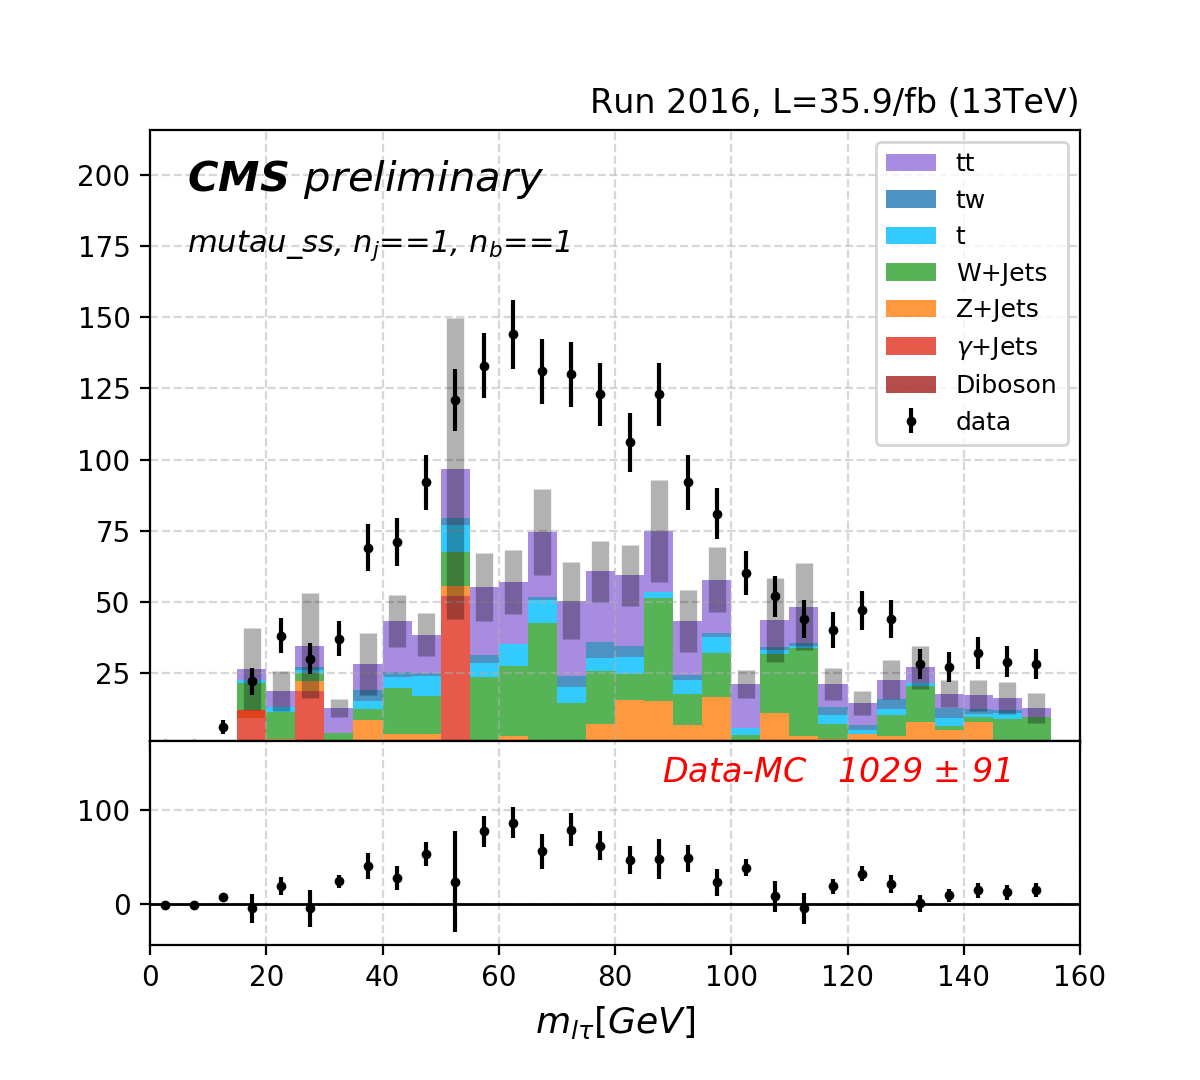
\includegraphics[width=0.24\textwidth]{chapters/Appendix/sectionQCD/figures/mutau_ss_==1_==1_dilepton_mass.png}
    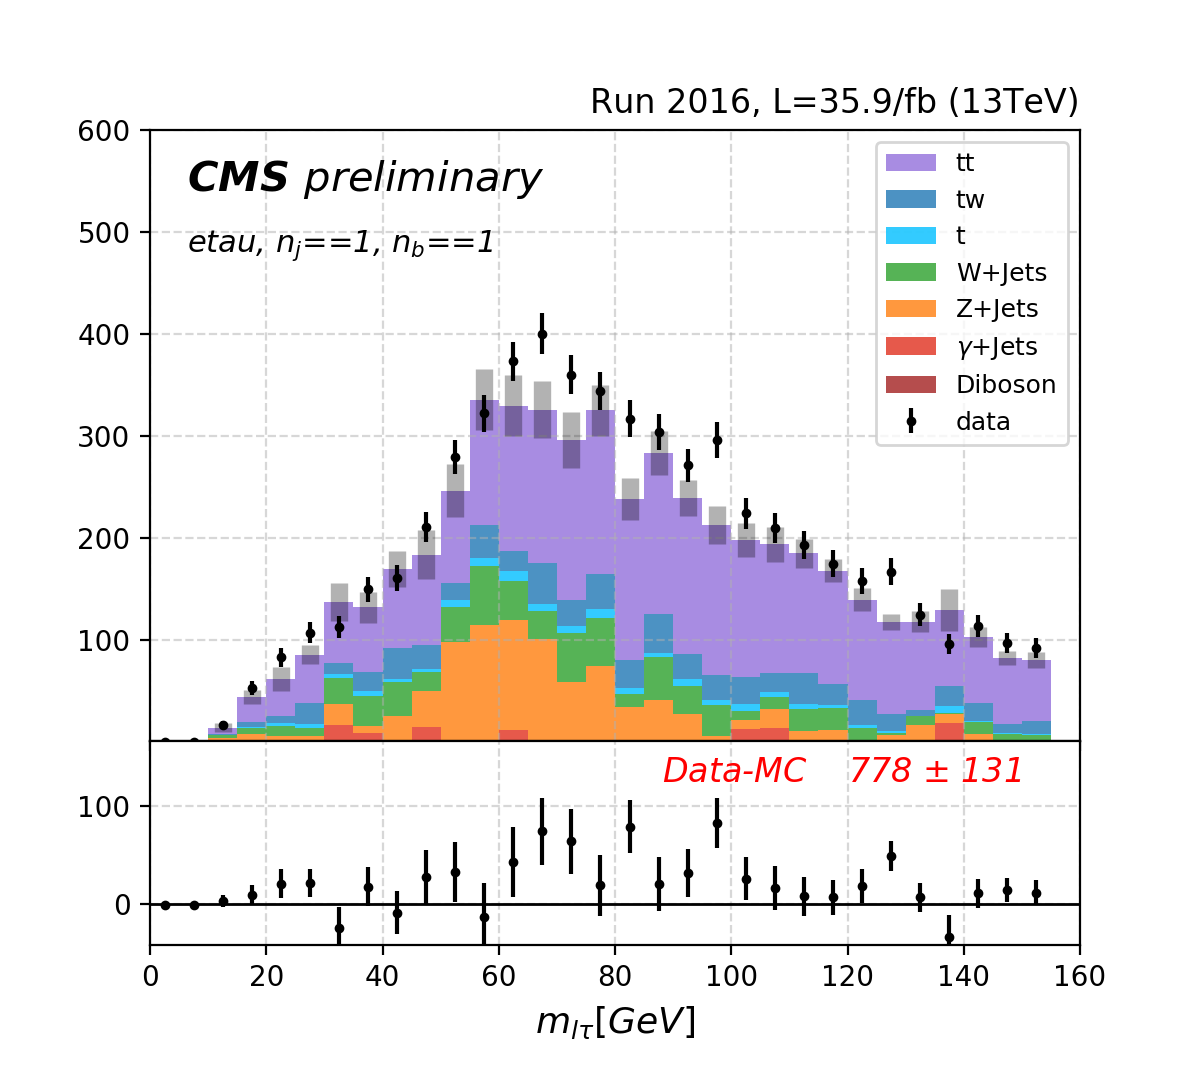
\includegraphics[width=0.24\textwidth]{chapters/Appendix/sectionQCD/figures/etau_==1_==1_dilepton_mass.png}
    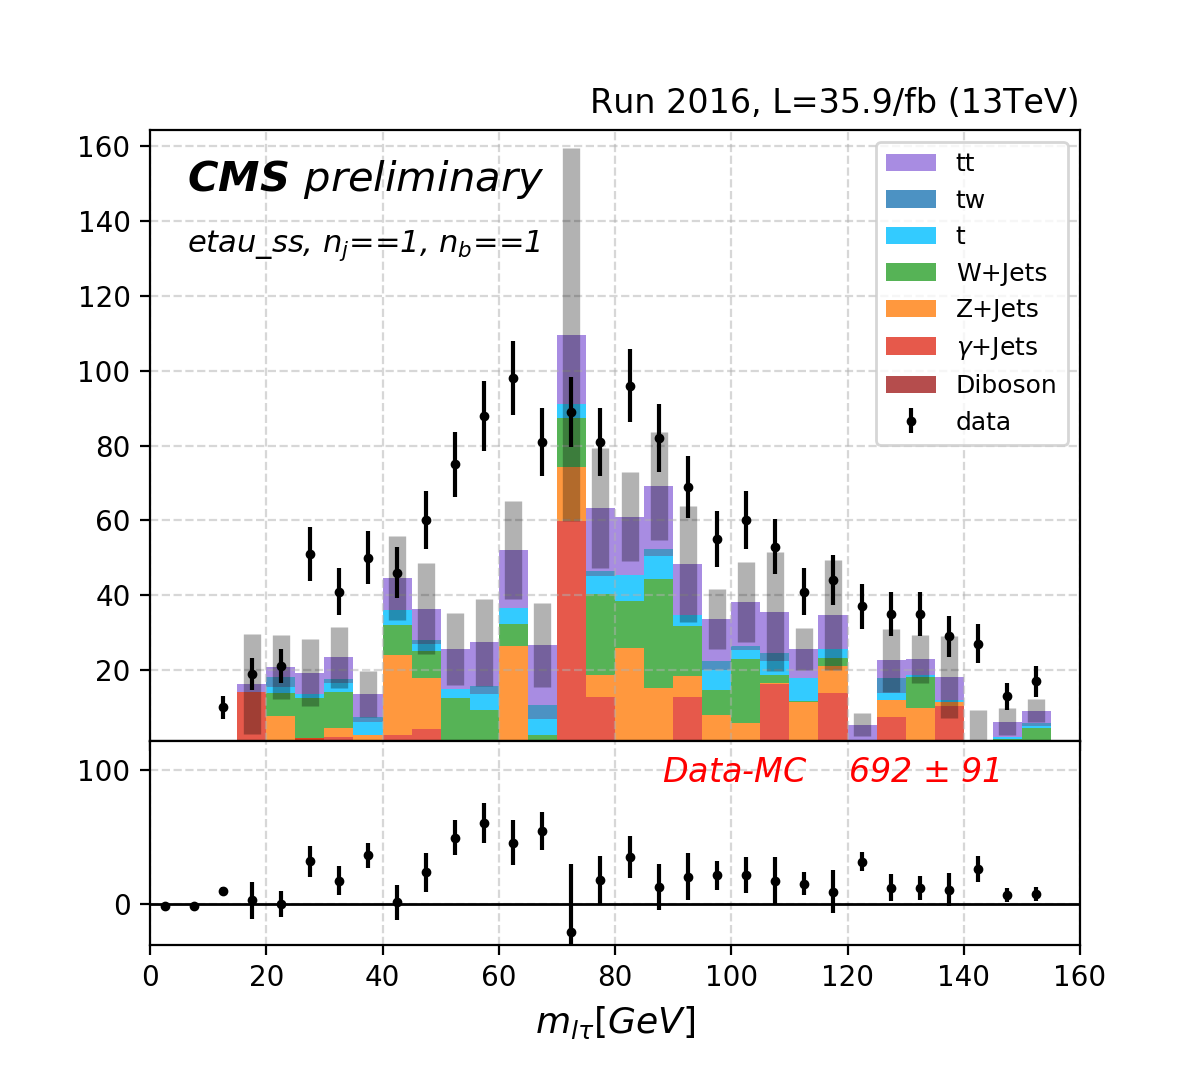
\includegraphics[width=0.24\textwidth]{chapters/Appendix/sectionQCD/figures/etau_ss_==1_==1_dilepton_mass.png}
    
    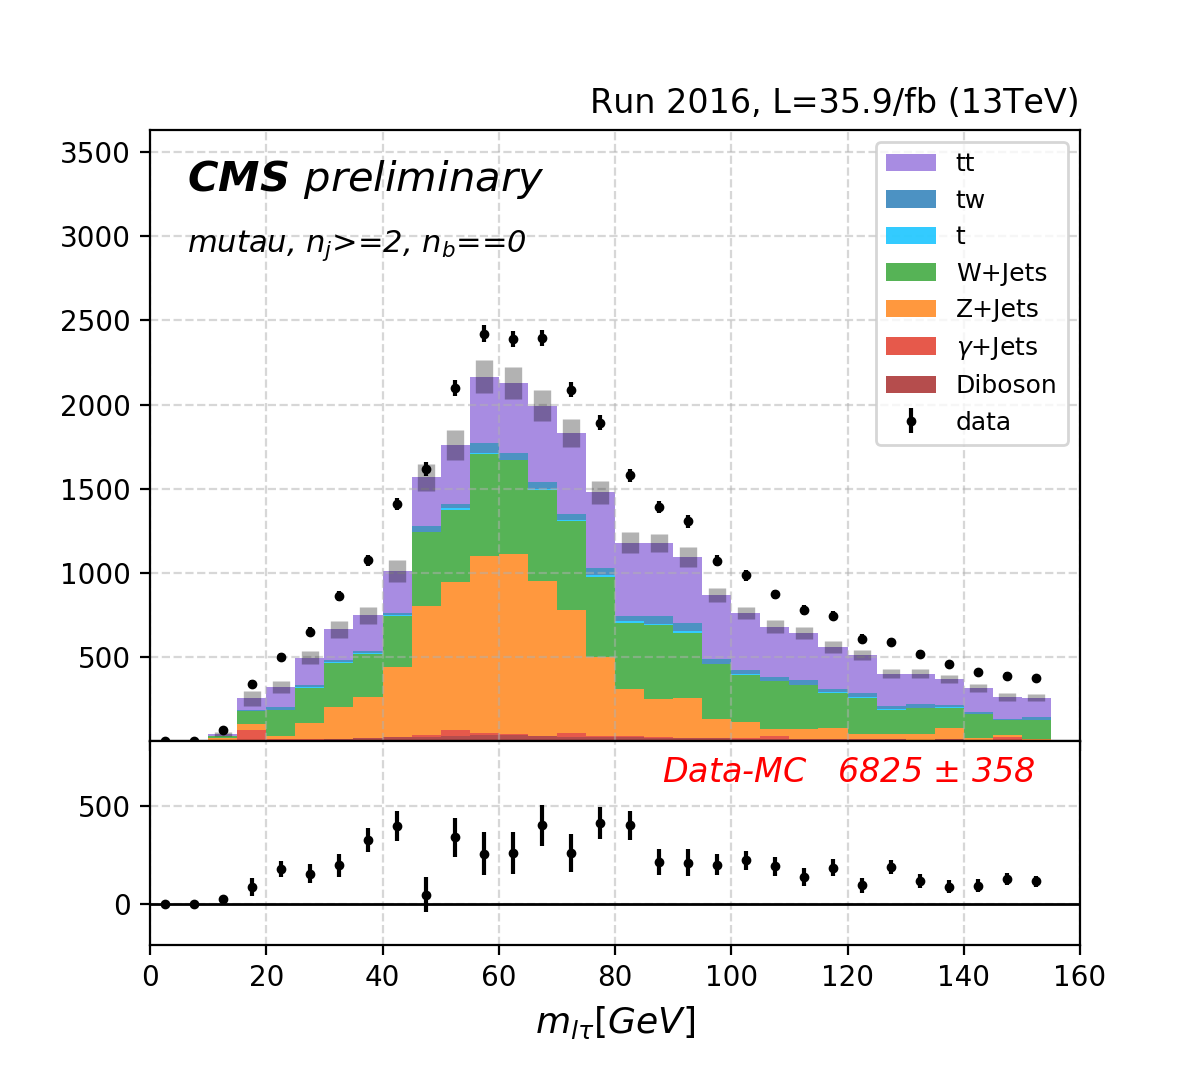
\includegraphics[width=0.24\textwidth]{chapters/Appendix/sectionQCD/figures/mutau_>=2_==0_dilepton_mass.png}
    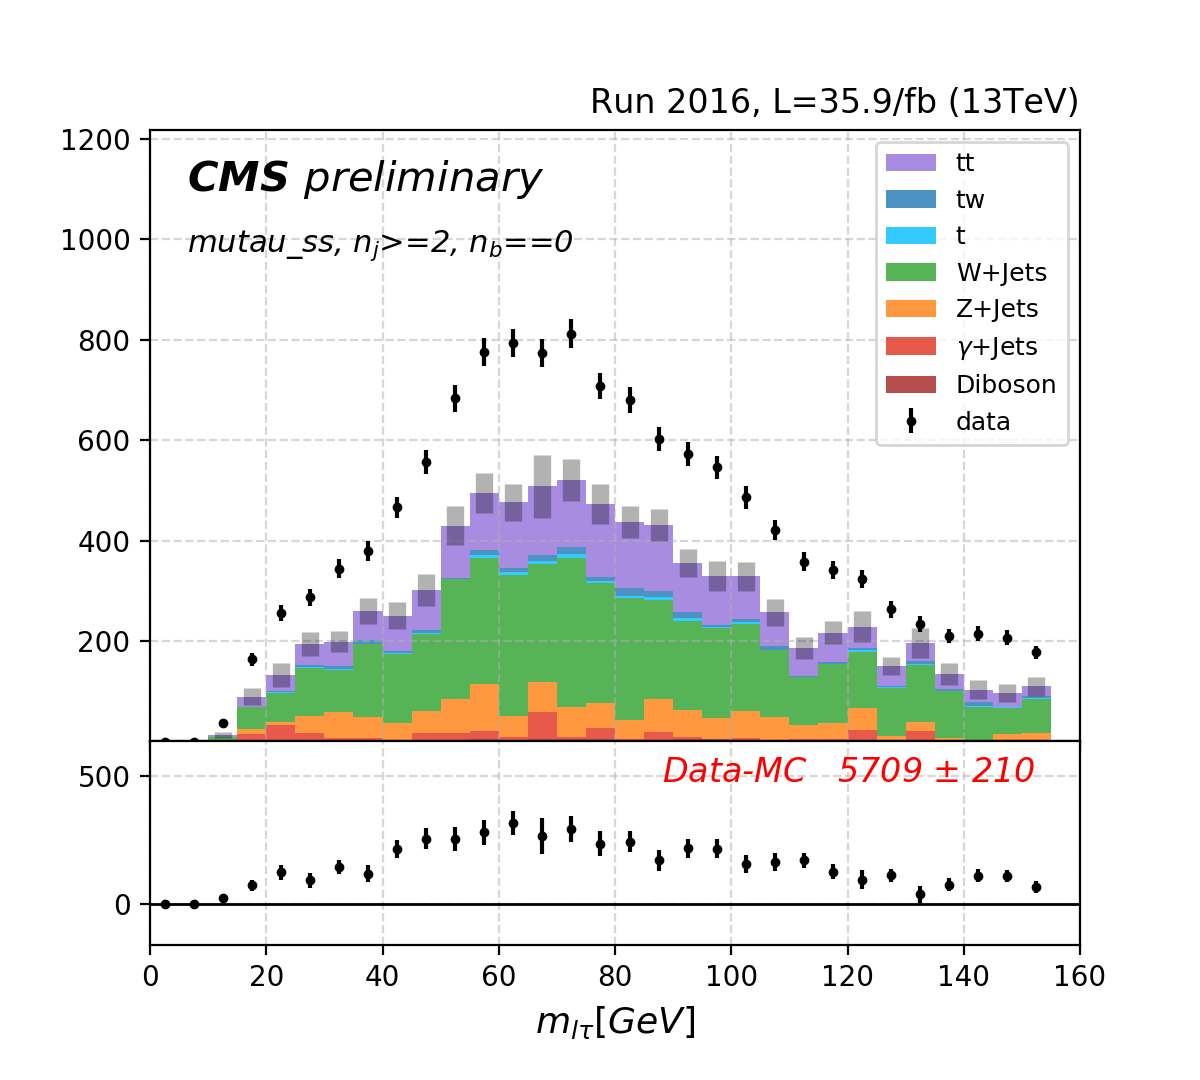
\includegraphics[width=0.24\textwidth]{chapters/Appendix/sectionQCD/figures/mutau_ss_>=2_==0_dilepton_mass.png}
    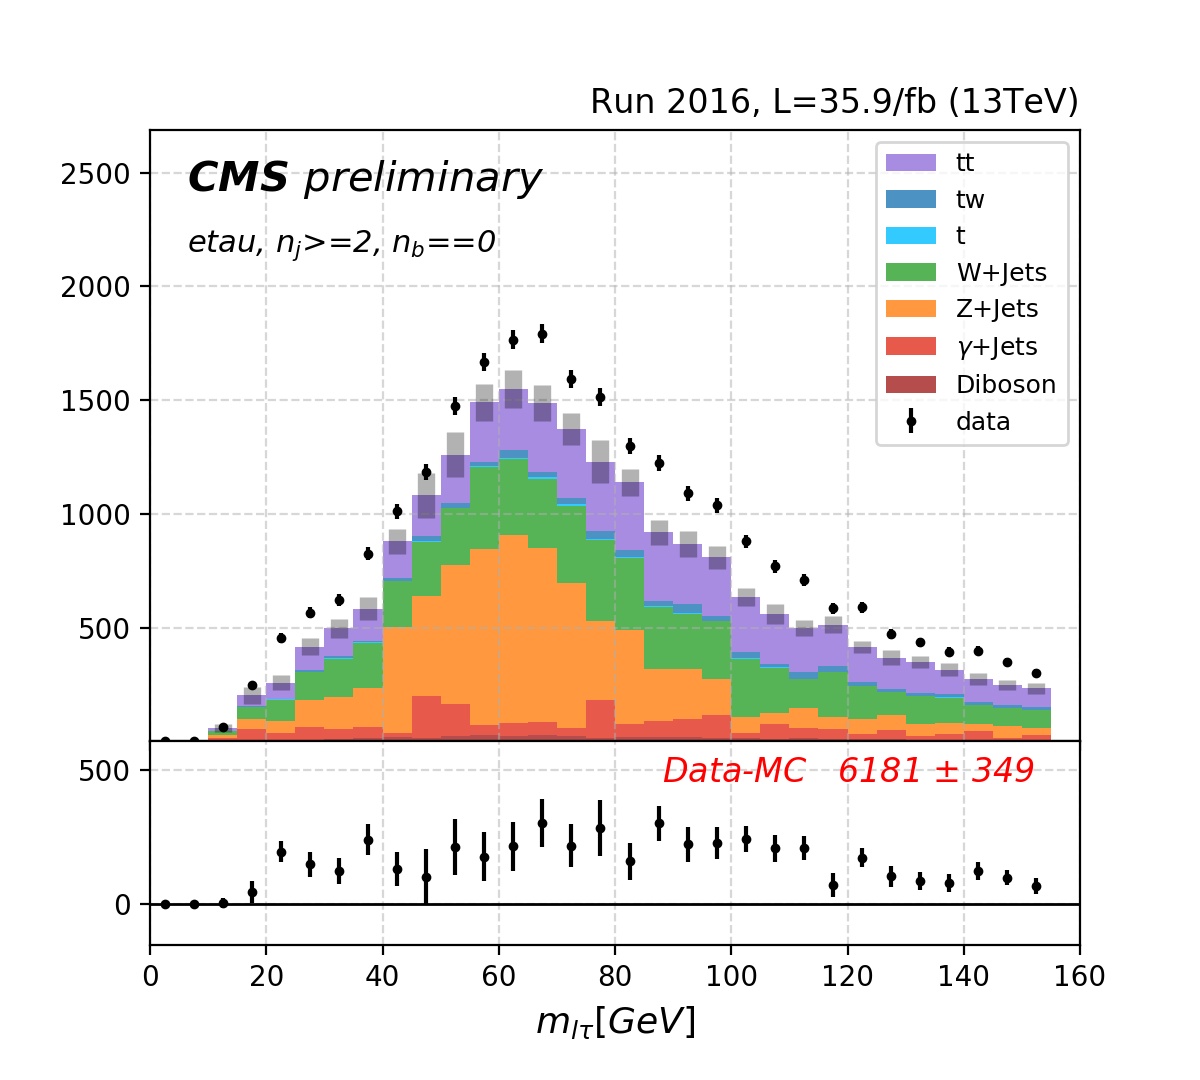
\includegraphics[width=0.24\textwidth]{chapters/Appendix/sectionQCD/figures/etau_>=2_==0_dilepton_mass.png}
    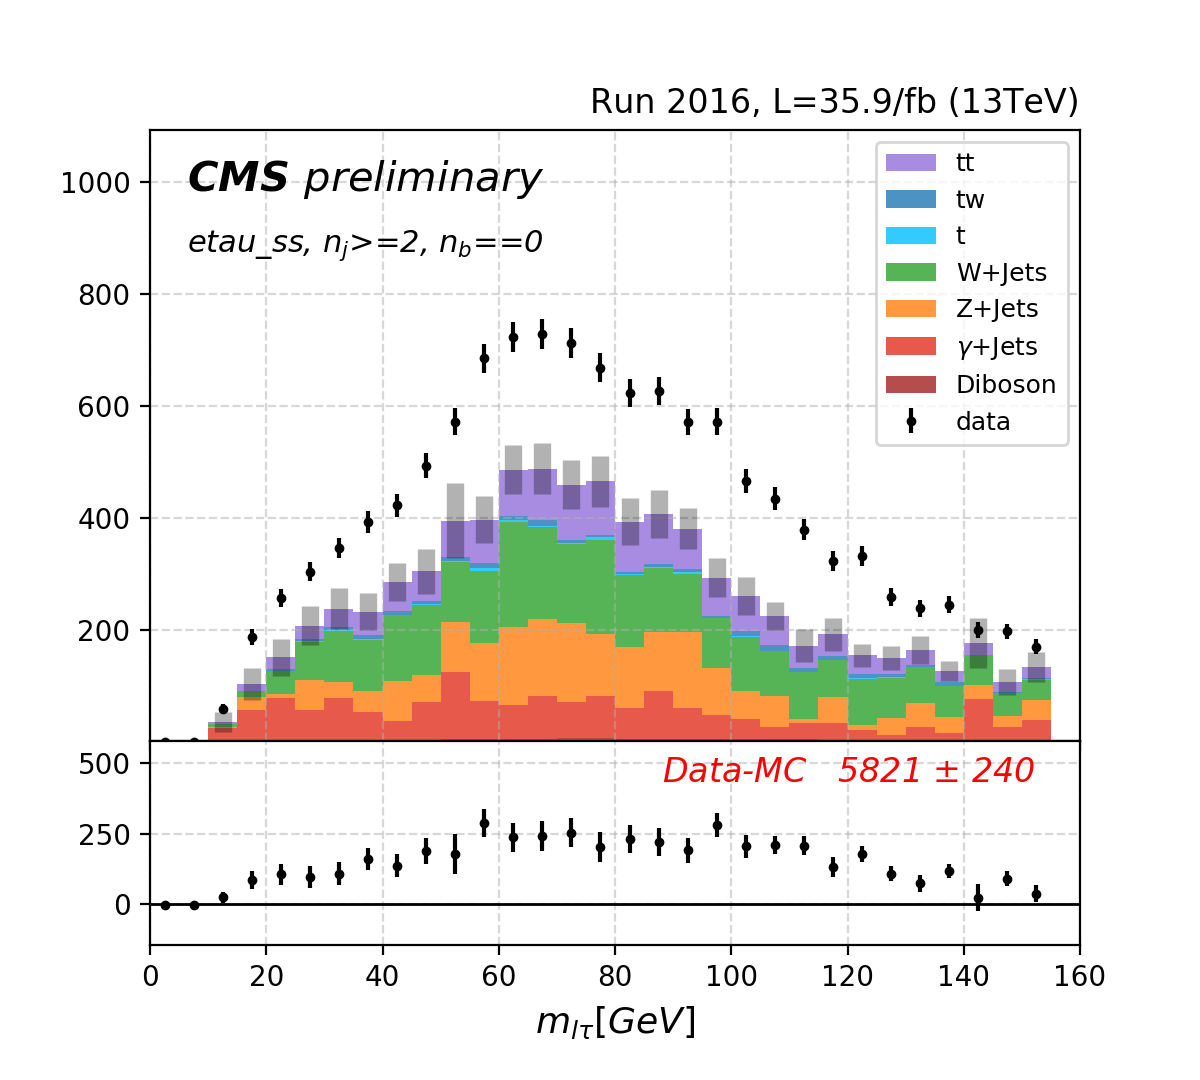
\includegraphics[width=0.24\textwidth]{chapters/Appendix/sectionQCD/figures/etau_ss_>=2_==0_dilepton_mass.png}
    
    
    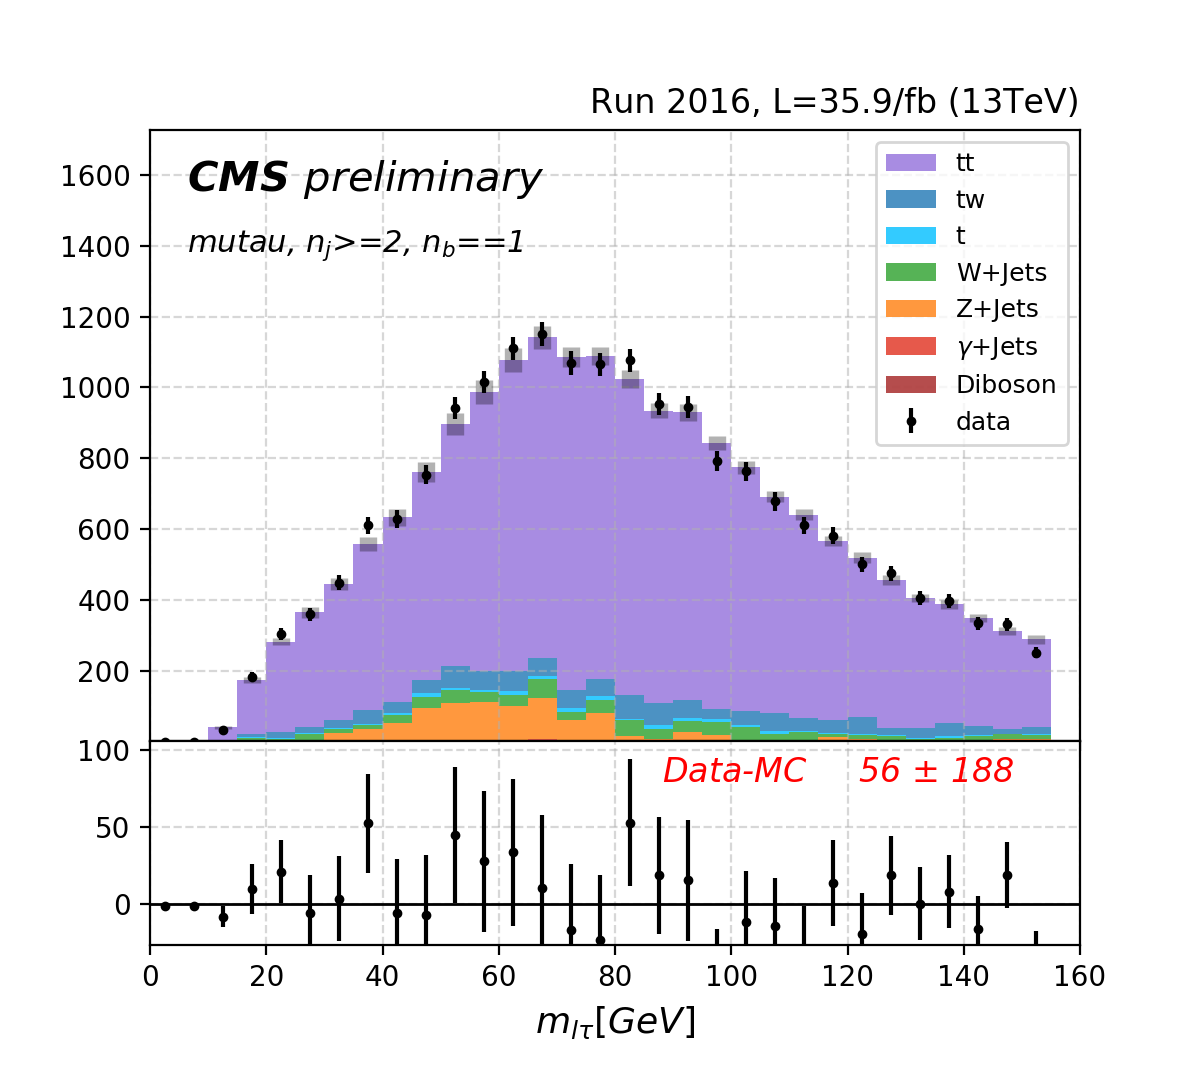
\includegraphics[width=0.24\textwidth]{chapters/Appendix/sectionQCD/figures/mutau_>=2_==1_dilepton_mass.png}
    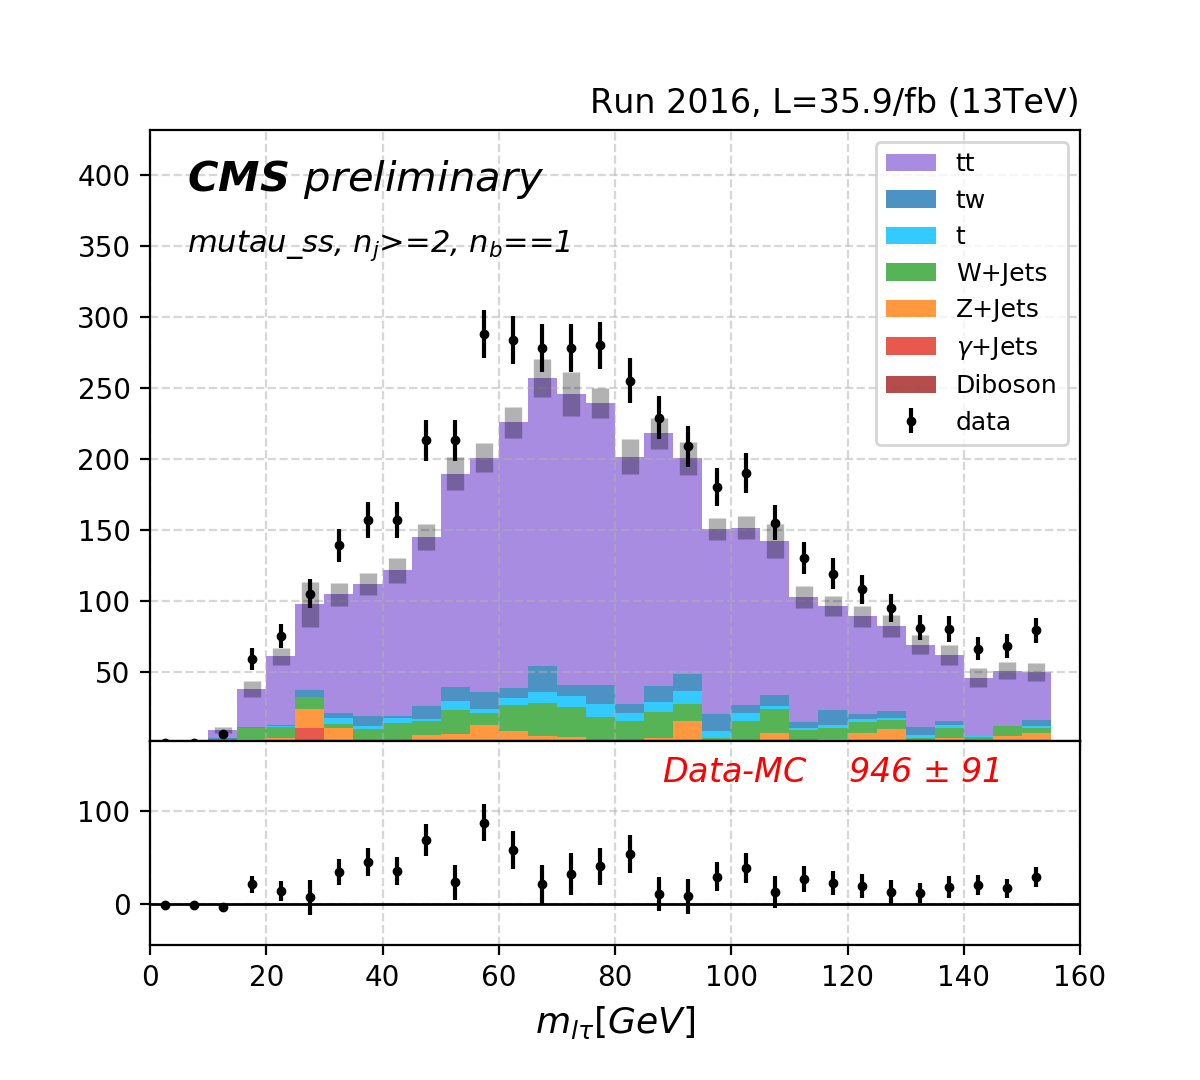
\includegraphics[width=0.24\textwidth]{chapters/Appendix/sectionQCD/figures/mutau_ss_>=2_==1_dilepton_mass.png}
    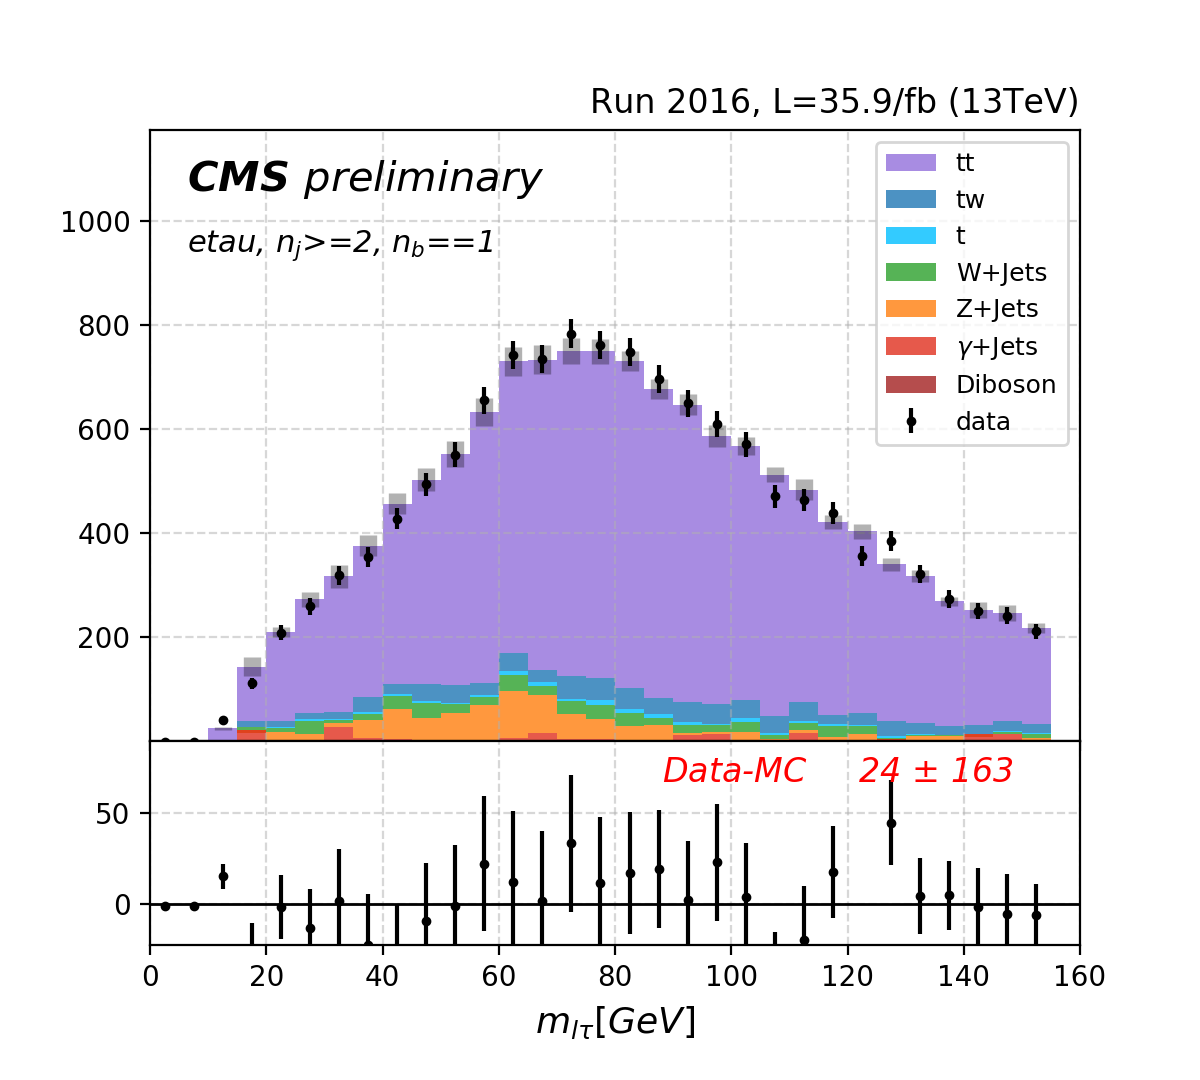
\includegraphics[width=0.24\textwidth]{chapters/Appendix/sectionQCD/figures/etau_>=2_==1_dilepton_mass.png}
    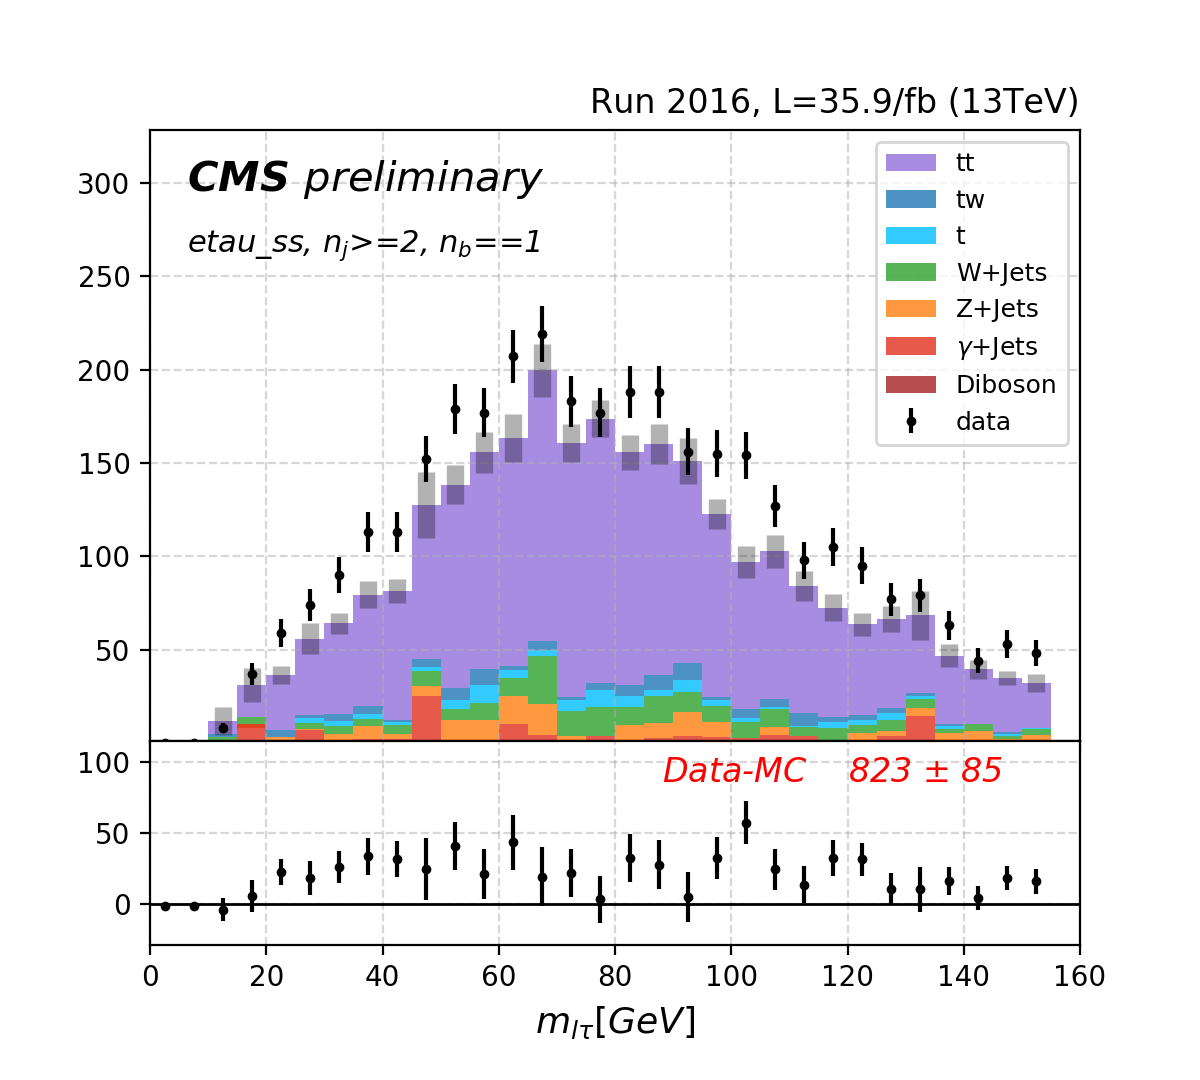
\includegraphics[width=0.24\textwidth]{chapters/Appendix/sectionQCD/figures/etau_ss_>=2_==1_dilepton_mass.png}
    
    
    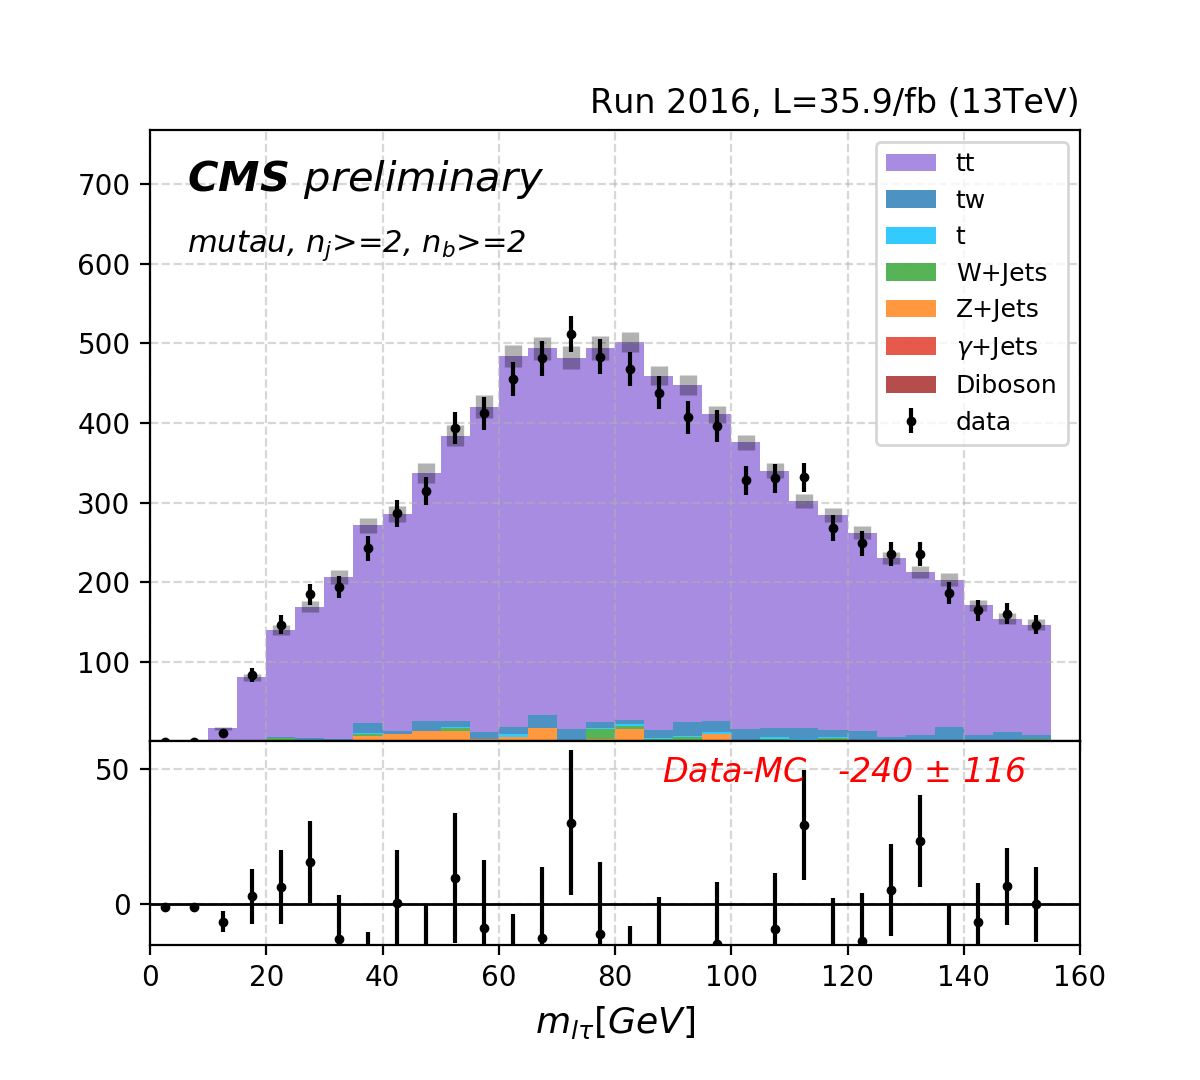
\includegraphics[width=0.24\textwidth]{chapters/Appendix/sectionQCD/figures/mutau_>=2_>=2_dilepton_mass.png}
    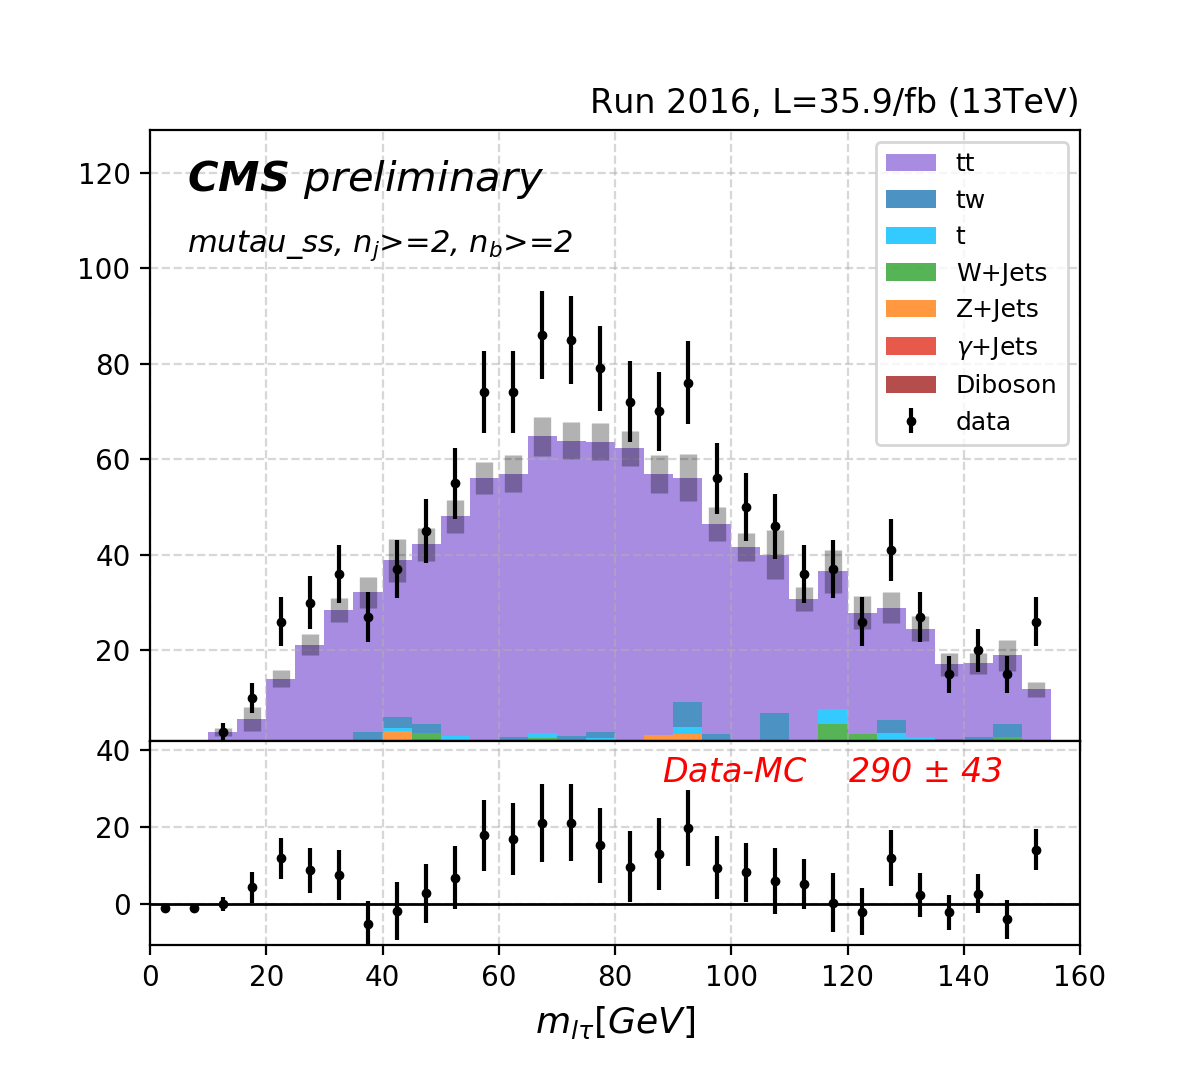
\includegraphics[width=0.24\textwidth]{chapters/Appendix/sectionQCD/figures/mutau_ss_>=2_>=2_dilepton_mass.png}
    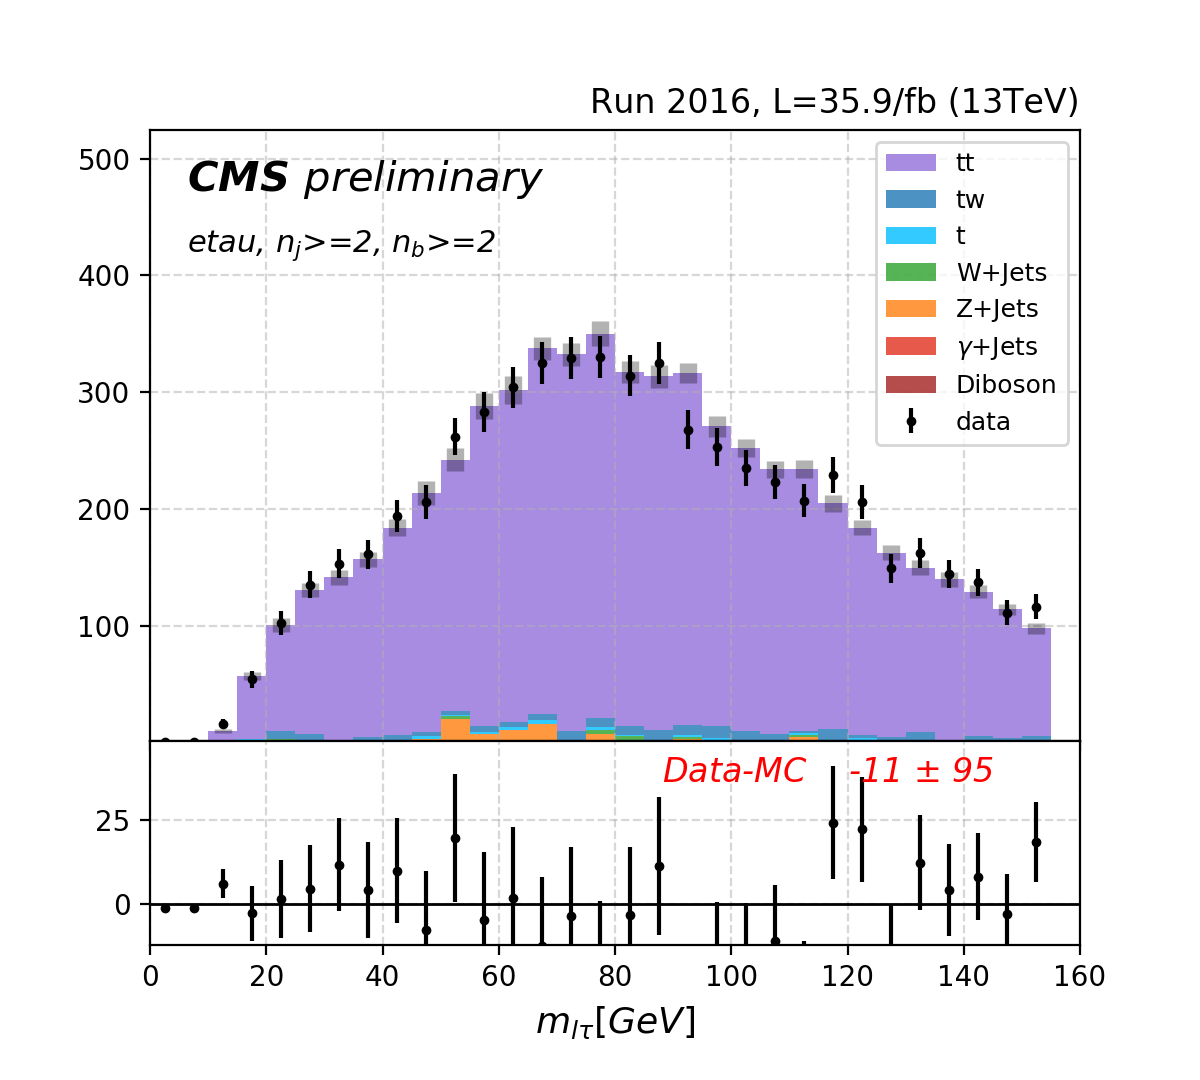
\includegraphics[width=0.24\textwidth]{chapters/Appendix/sectionQCD/figures/etau_>=2_>=2_dilepton_mass.png}
    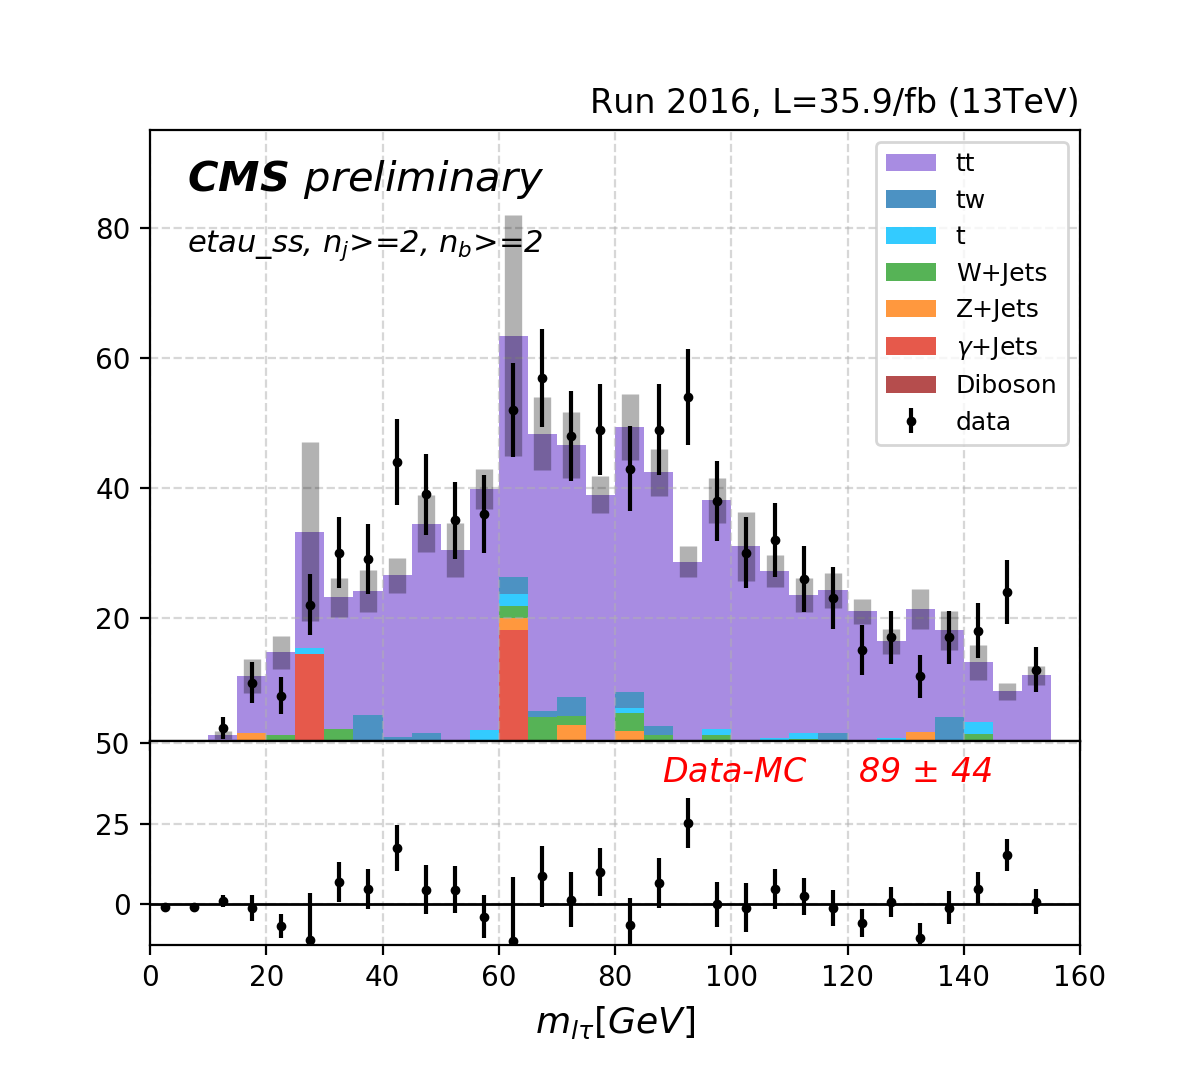
\includegraphics[width=0.24\textwidth]{chapters/Appendix/sectionQCD/figures/etau_ss_>=2_>=2_dilepton_mass.png}
    
    

    \caption{The $m_{l\tau}$ in the SS and OS region of $\mu\tau$ (left two columns) and $e\tau$ (right two columns) 
    channel. Different rows correspond to different $n_j,n_b$ configuration, which includes
    $n_j=0,n_b=0$, $n_j=1,n_b=0$, $n_j=1,n_b=1$, $n_j\geq 2,n_b=0$, $n_j\geq 2,n_b=1$, $n_j\geq 2,n_b\geq 2$, 
    from the first to the last row. The last two rows dominated by \ttbar are the channels used by the counting analysis.
    }
    \label{fig:appendix:qcdsf:ltau}
\end{figure}



\begin{figure}
    \centering
    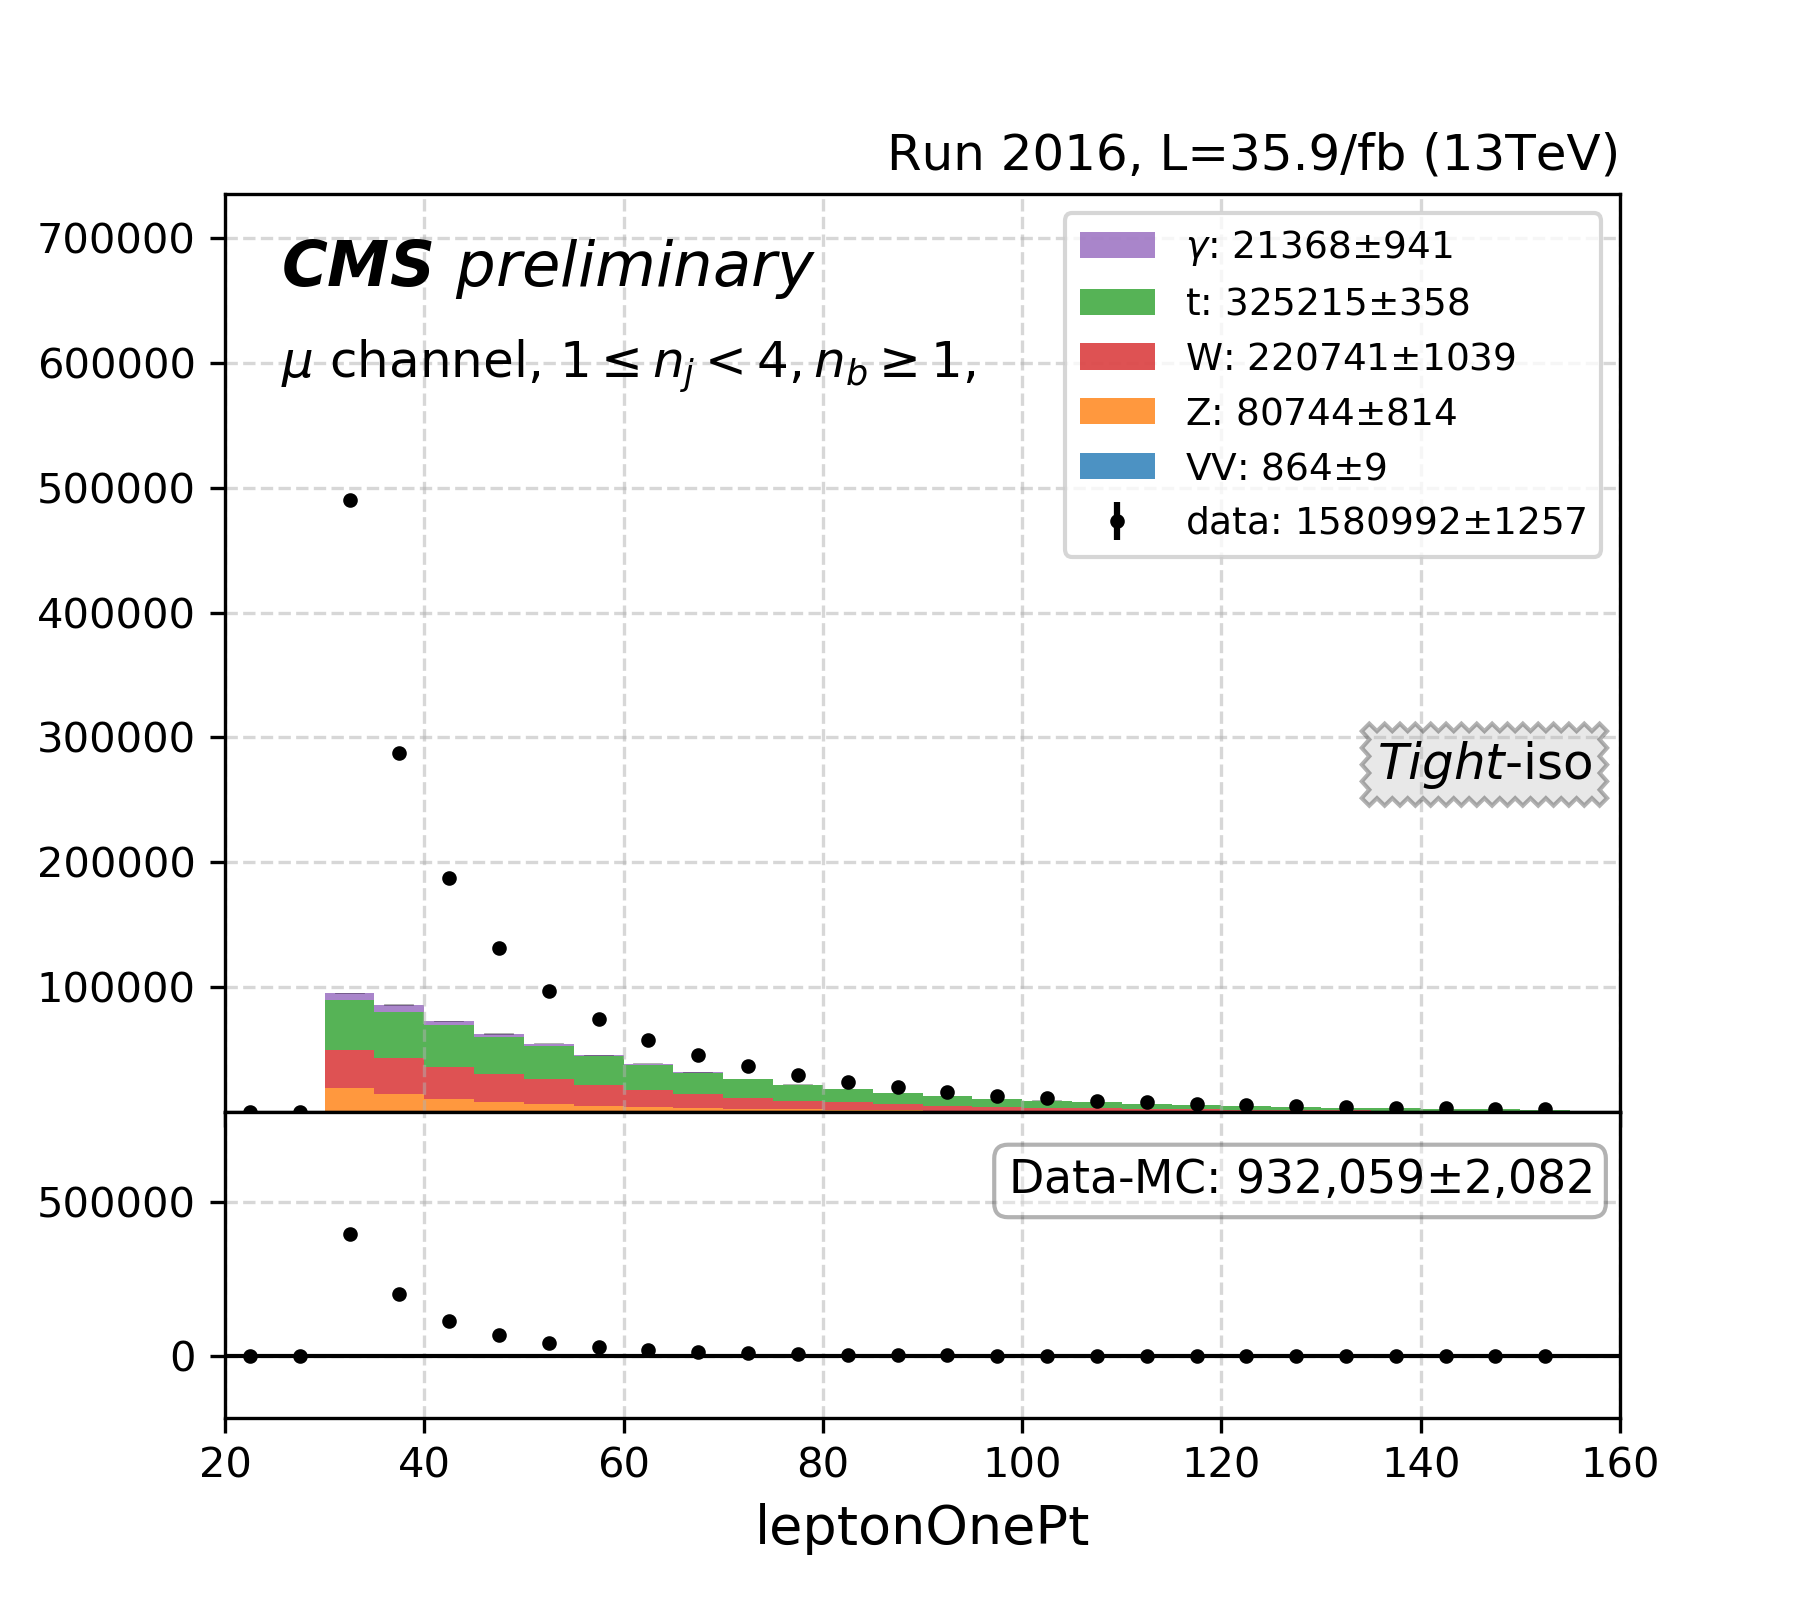
\includegraphics[width=0.24\textwidth]{chapters/Appendix/sectionQCD/figures/123j1b/mu_leptonOnePt_True.png}
    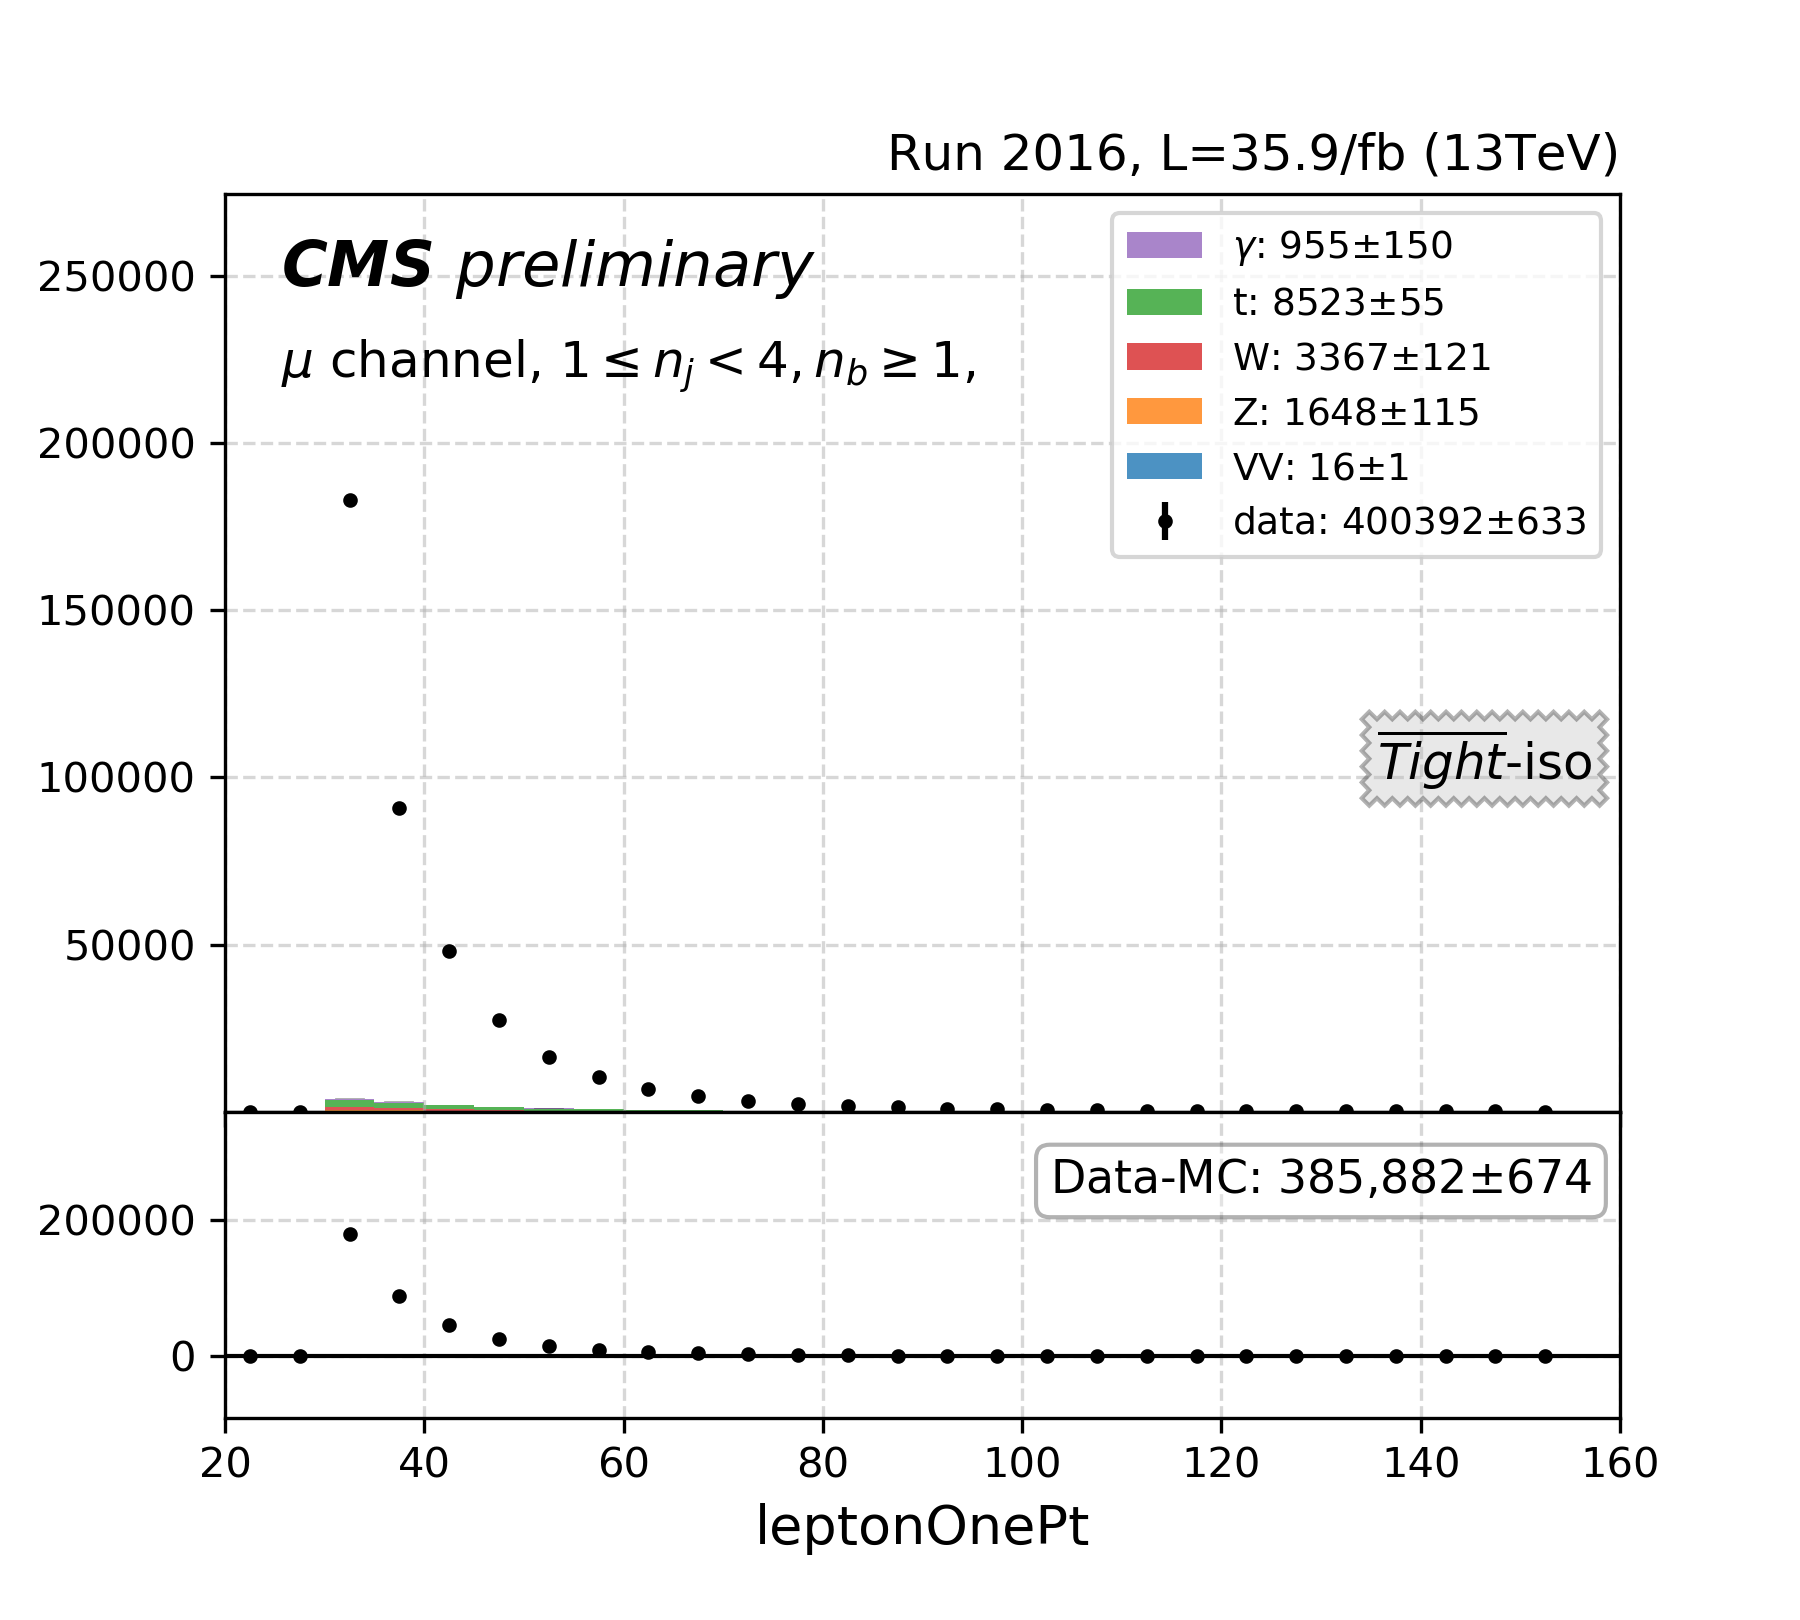
\includegraphics[width=0.24\textwidth]{chapters/Appendix/sectionQCD/figures/123j1b/mu_leptonOnePt_False.png}
    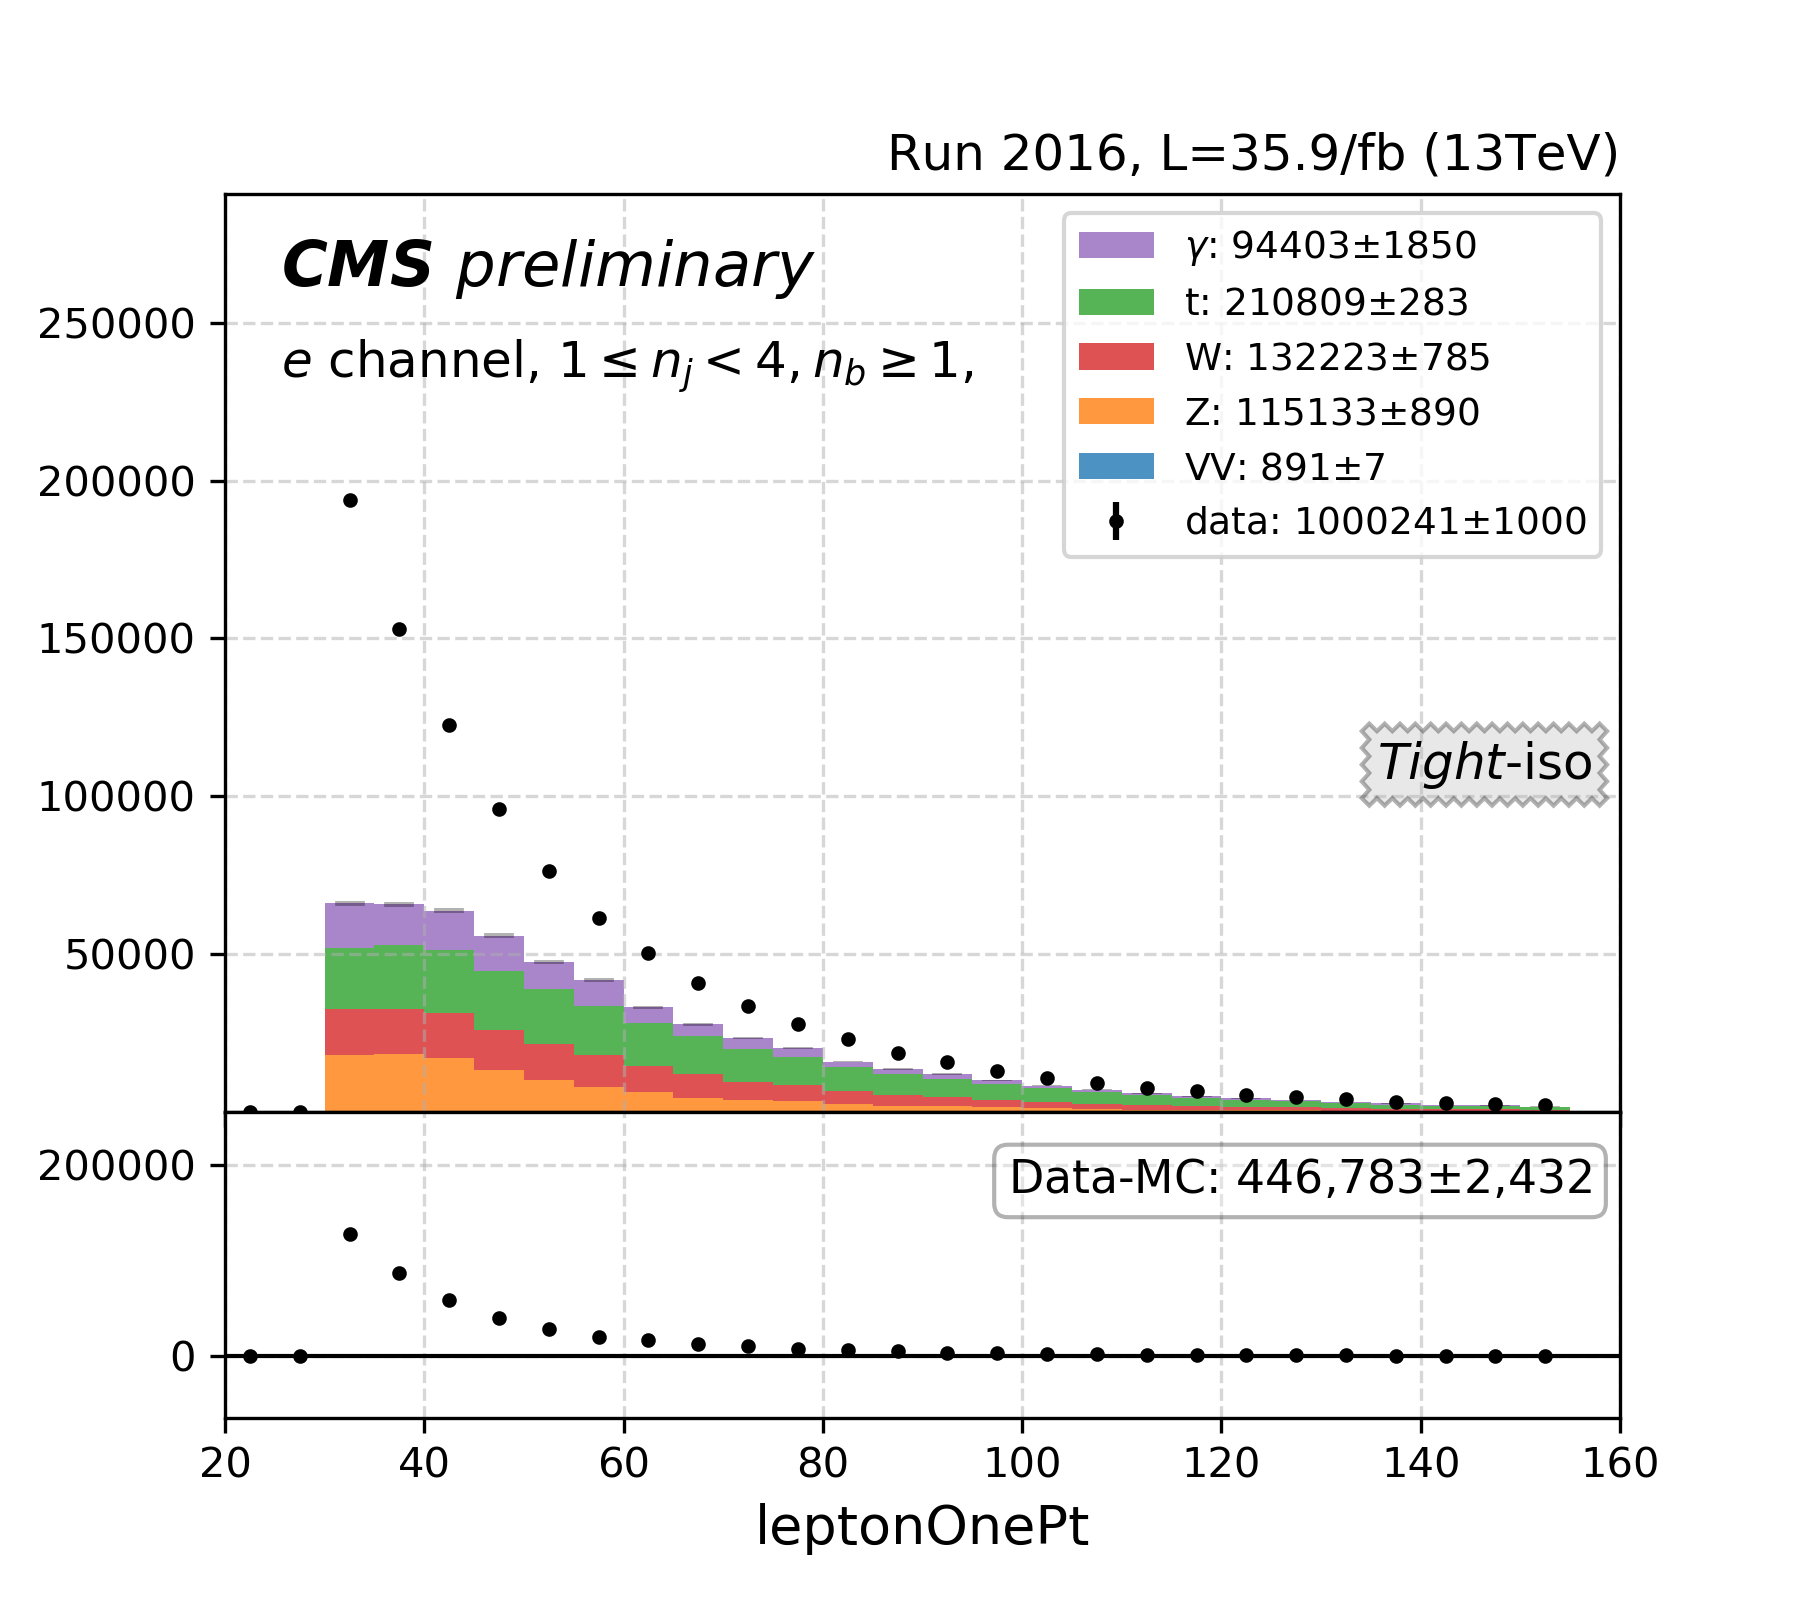
\includegraphics[width=0.24\textwidth]{chapters/Appendix/sectionQCD/figures/123j1b/e_leptonOnePt_True.png}
    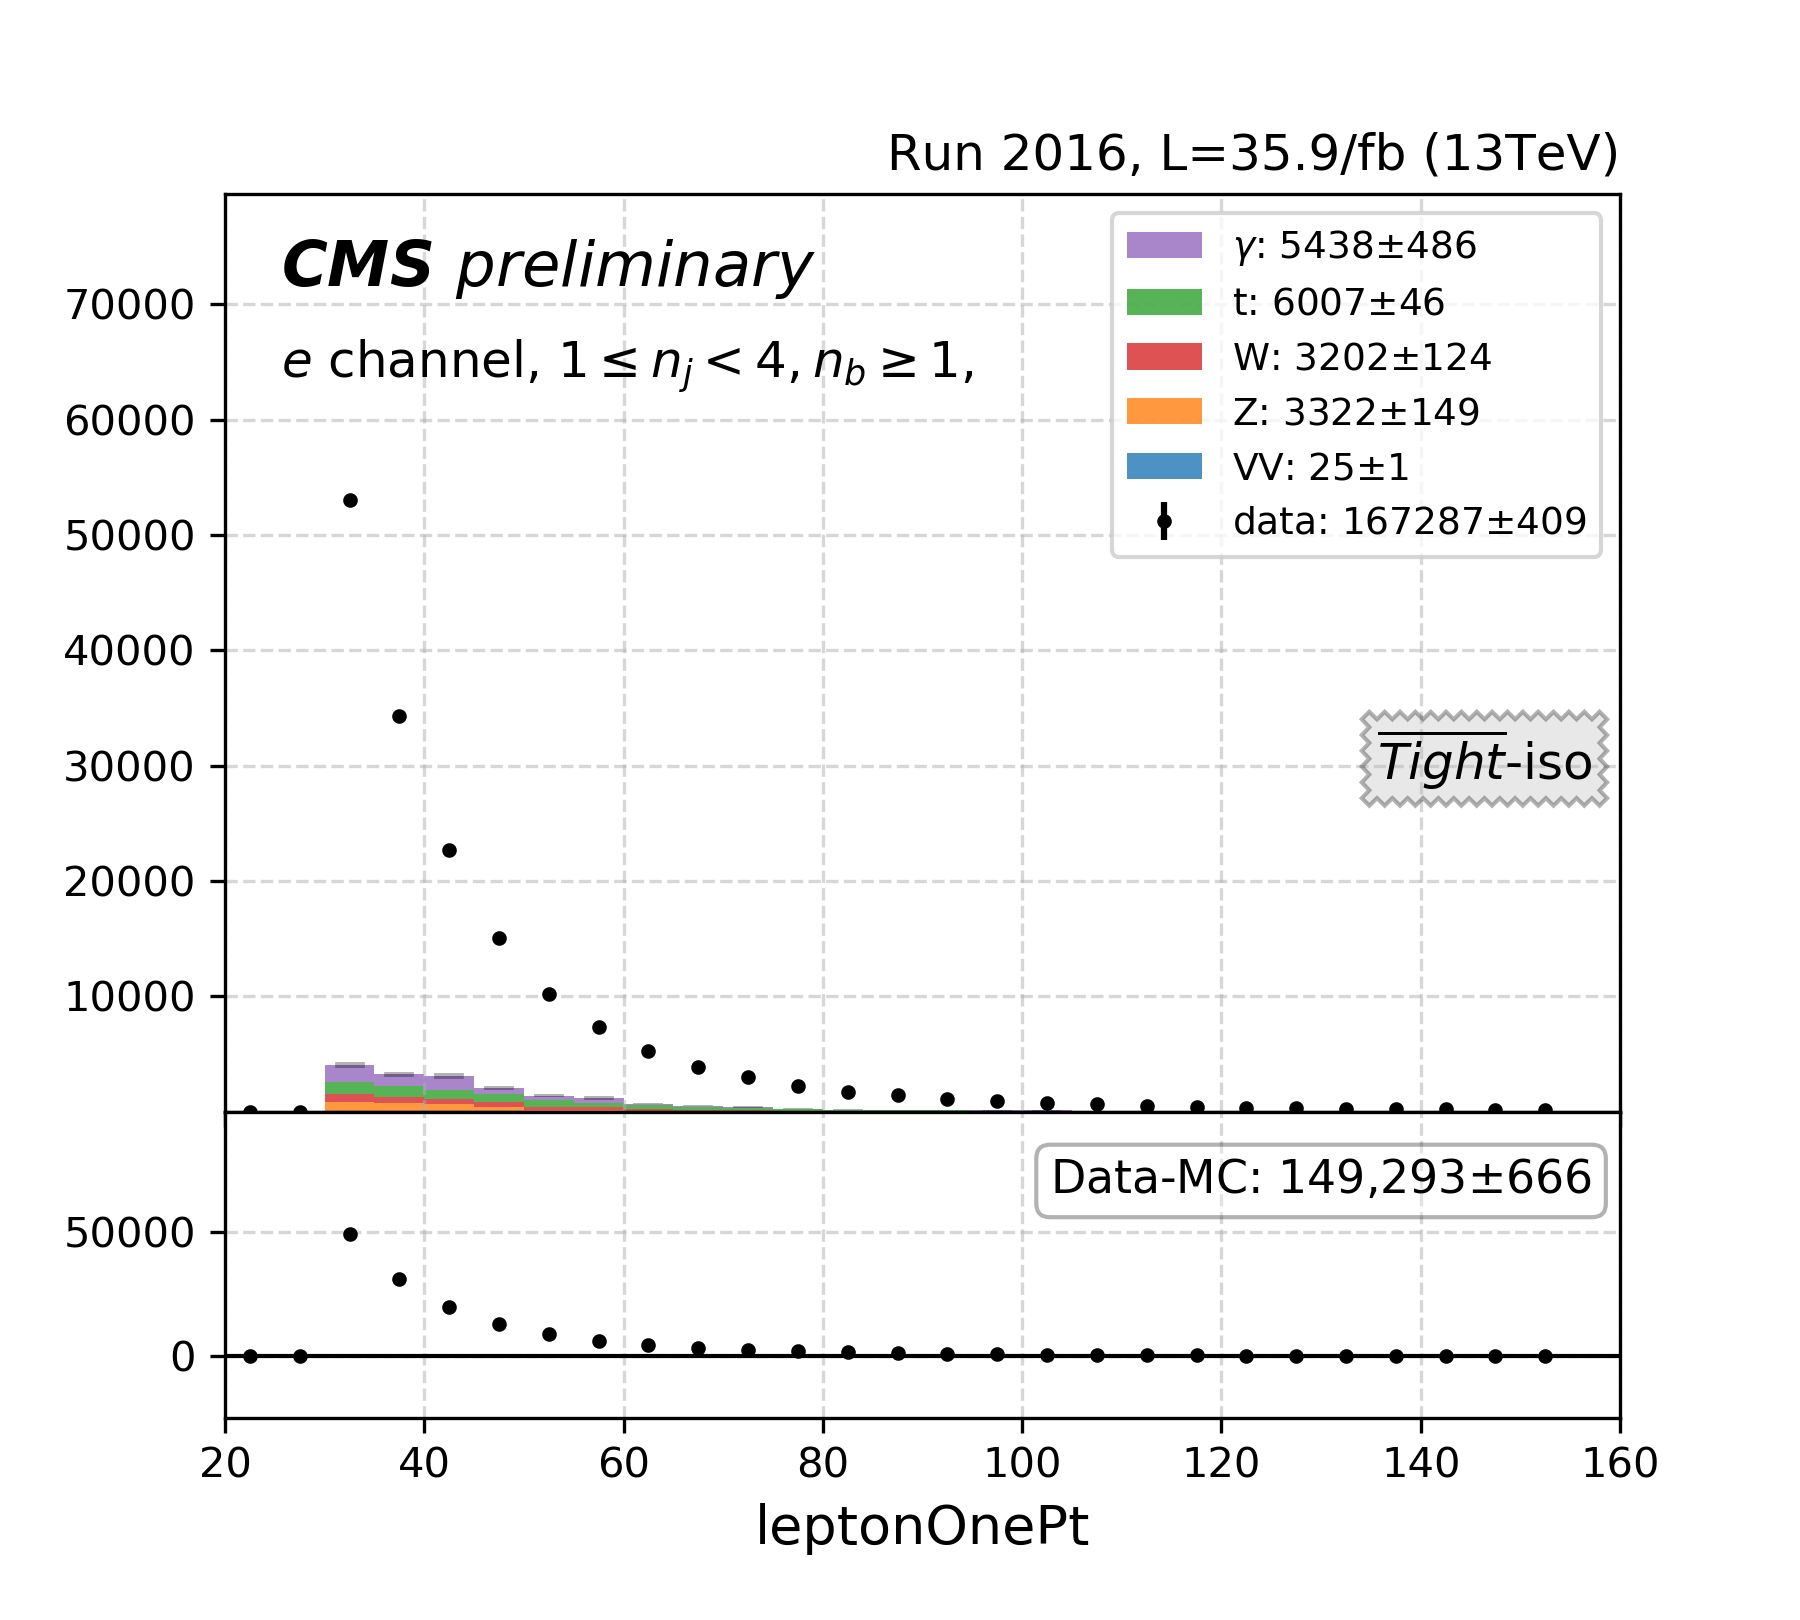
\includegraphics[width=0.24\textwidth]{chapters/Appendix/sectionQCD/figures/123j1b/e_leptonOnePt_False.png}
    
    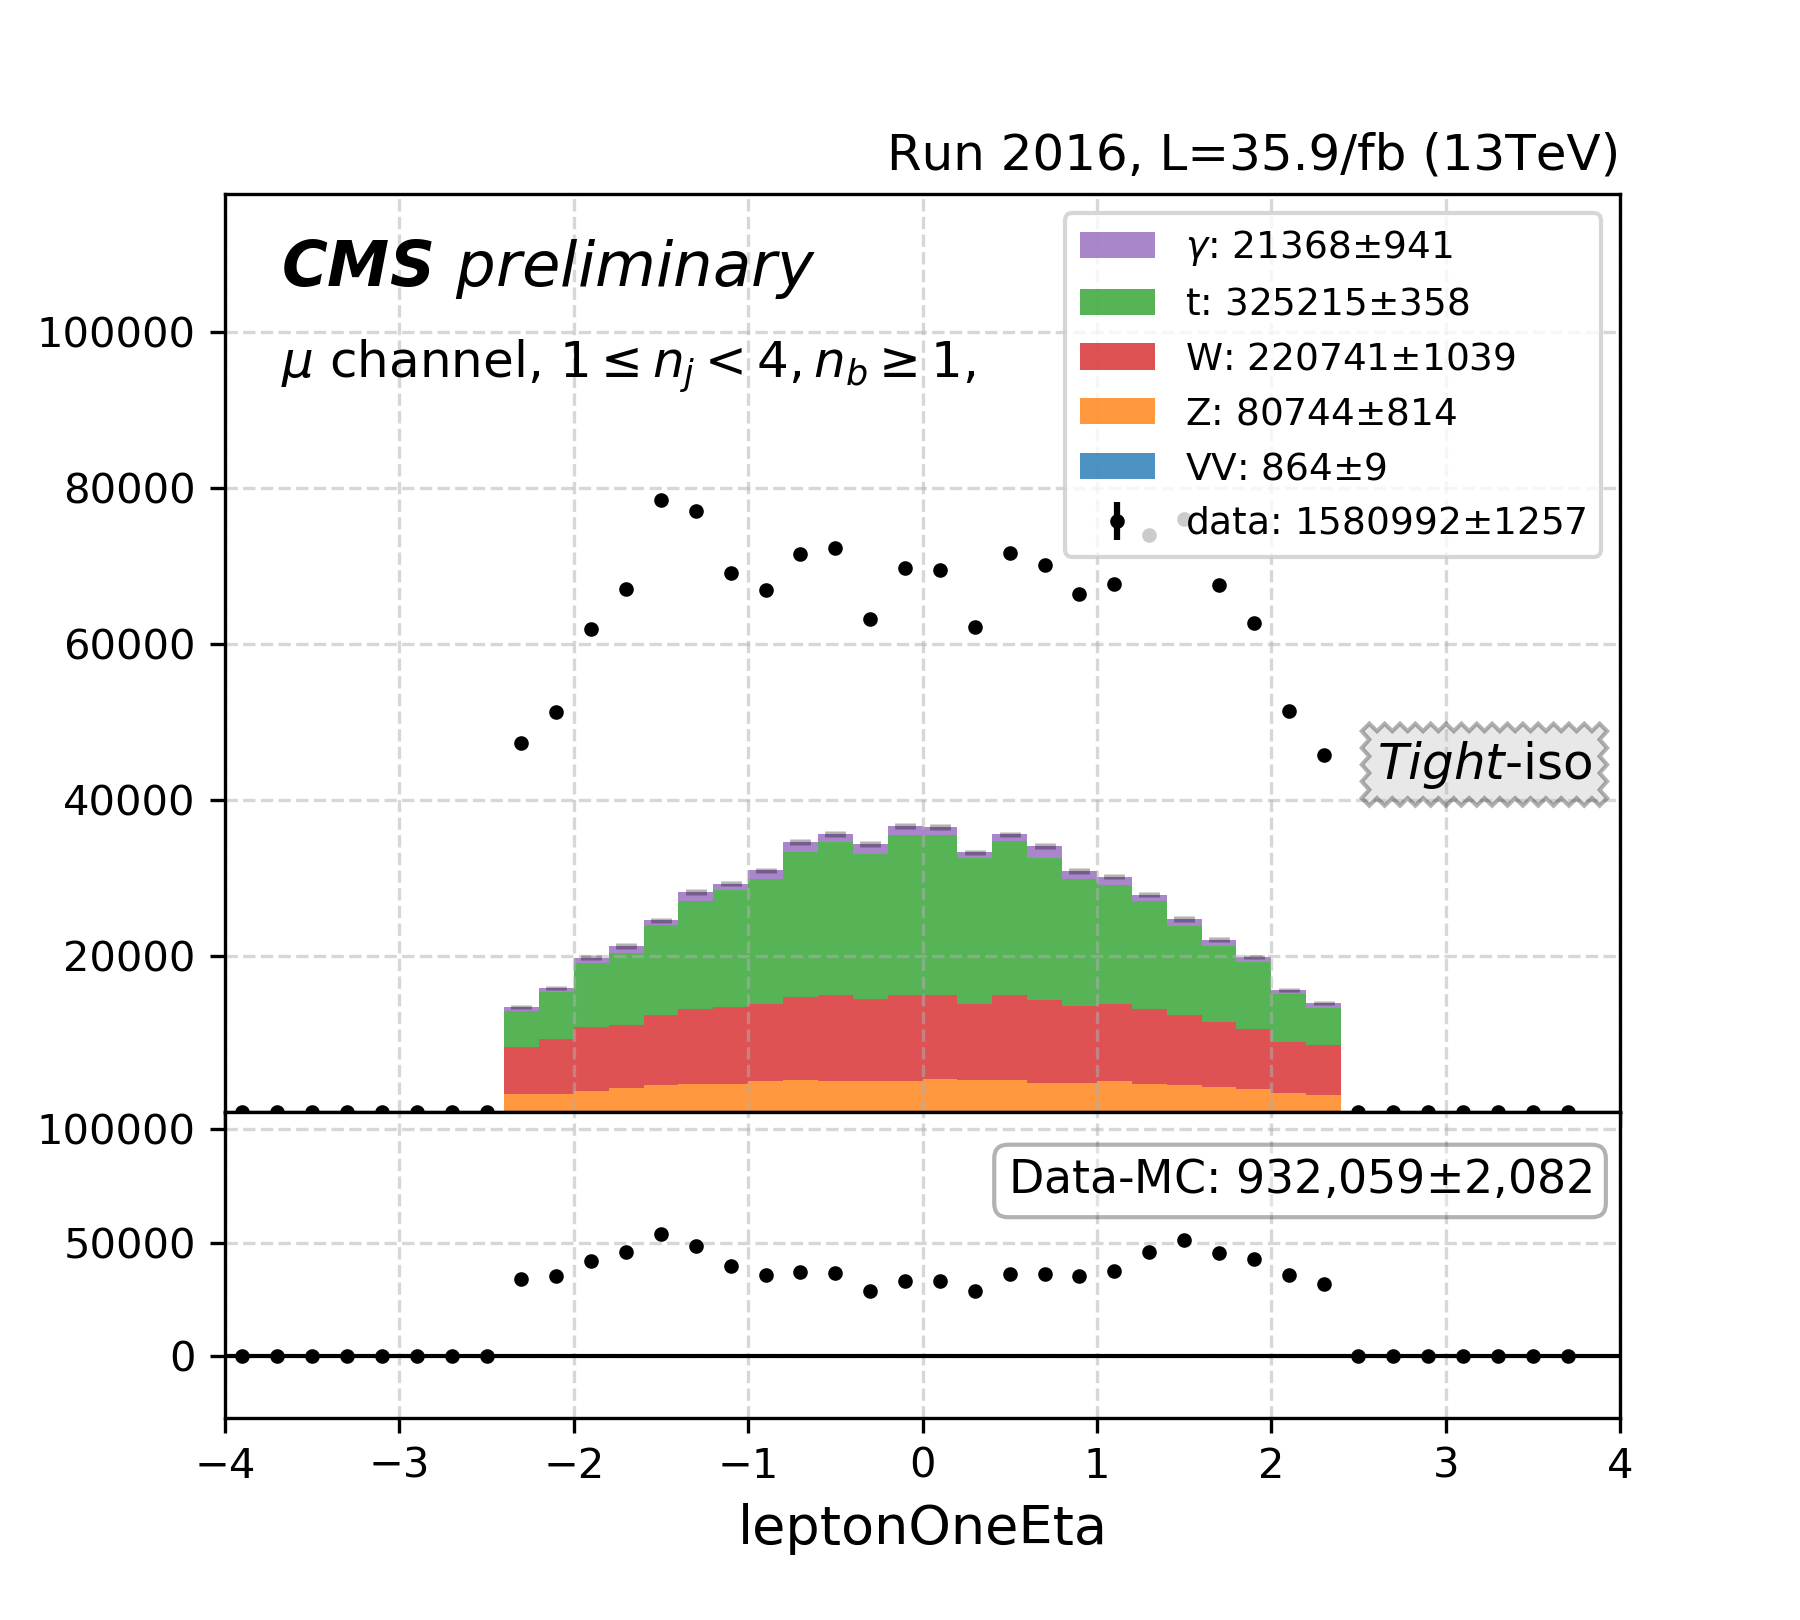
\includegraphics[width=0.24\textwidth]{chapters/Appendix/sectionQCD/figures/123j1b/mu_leptonOneEta_True.png}
    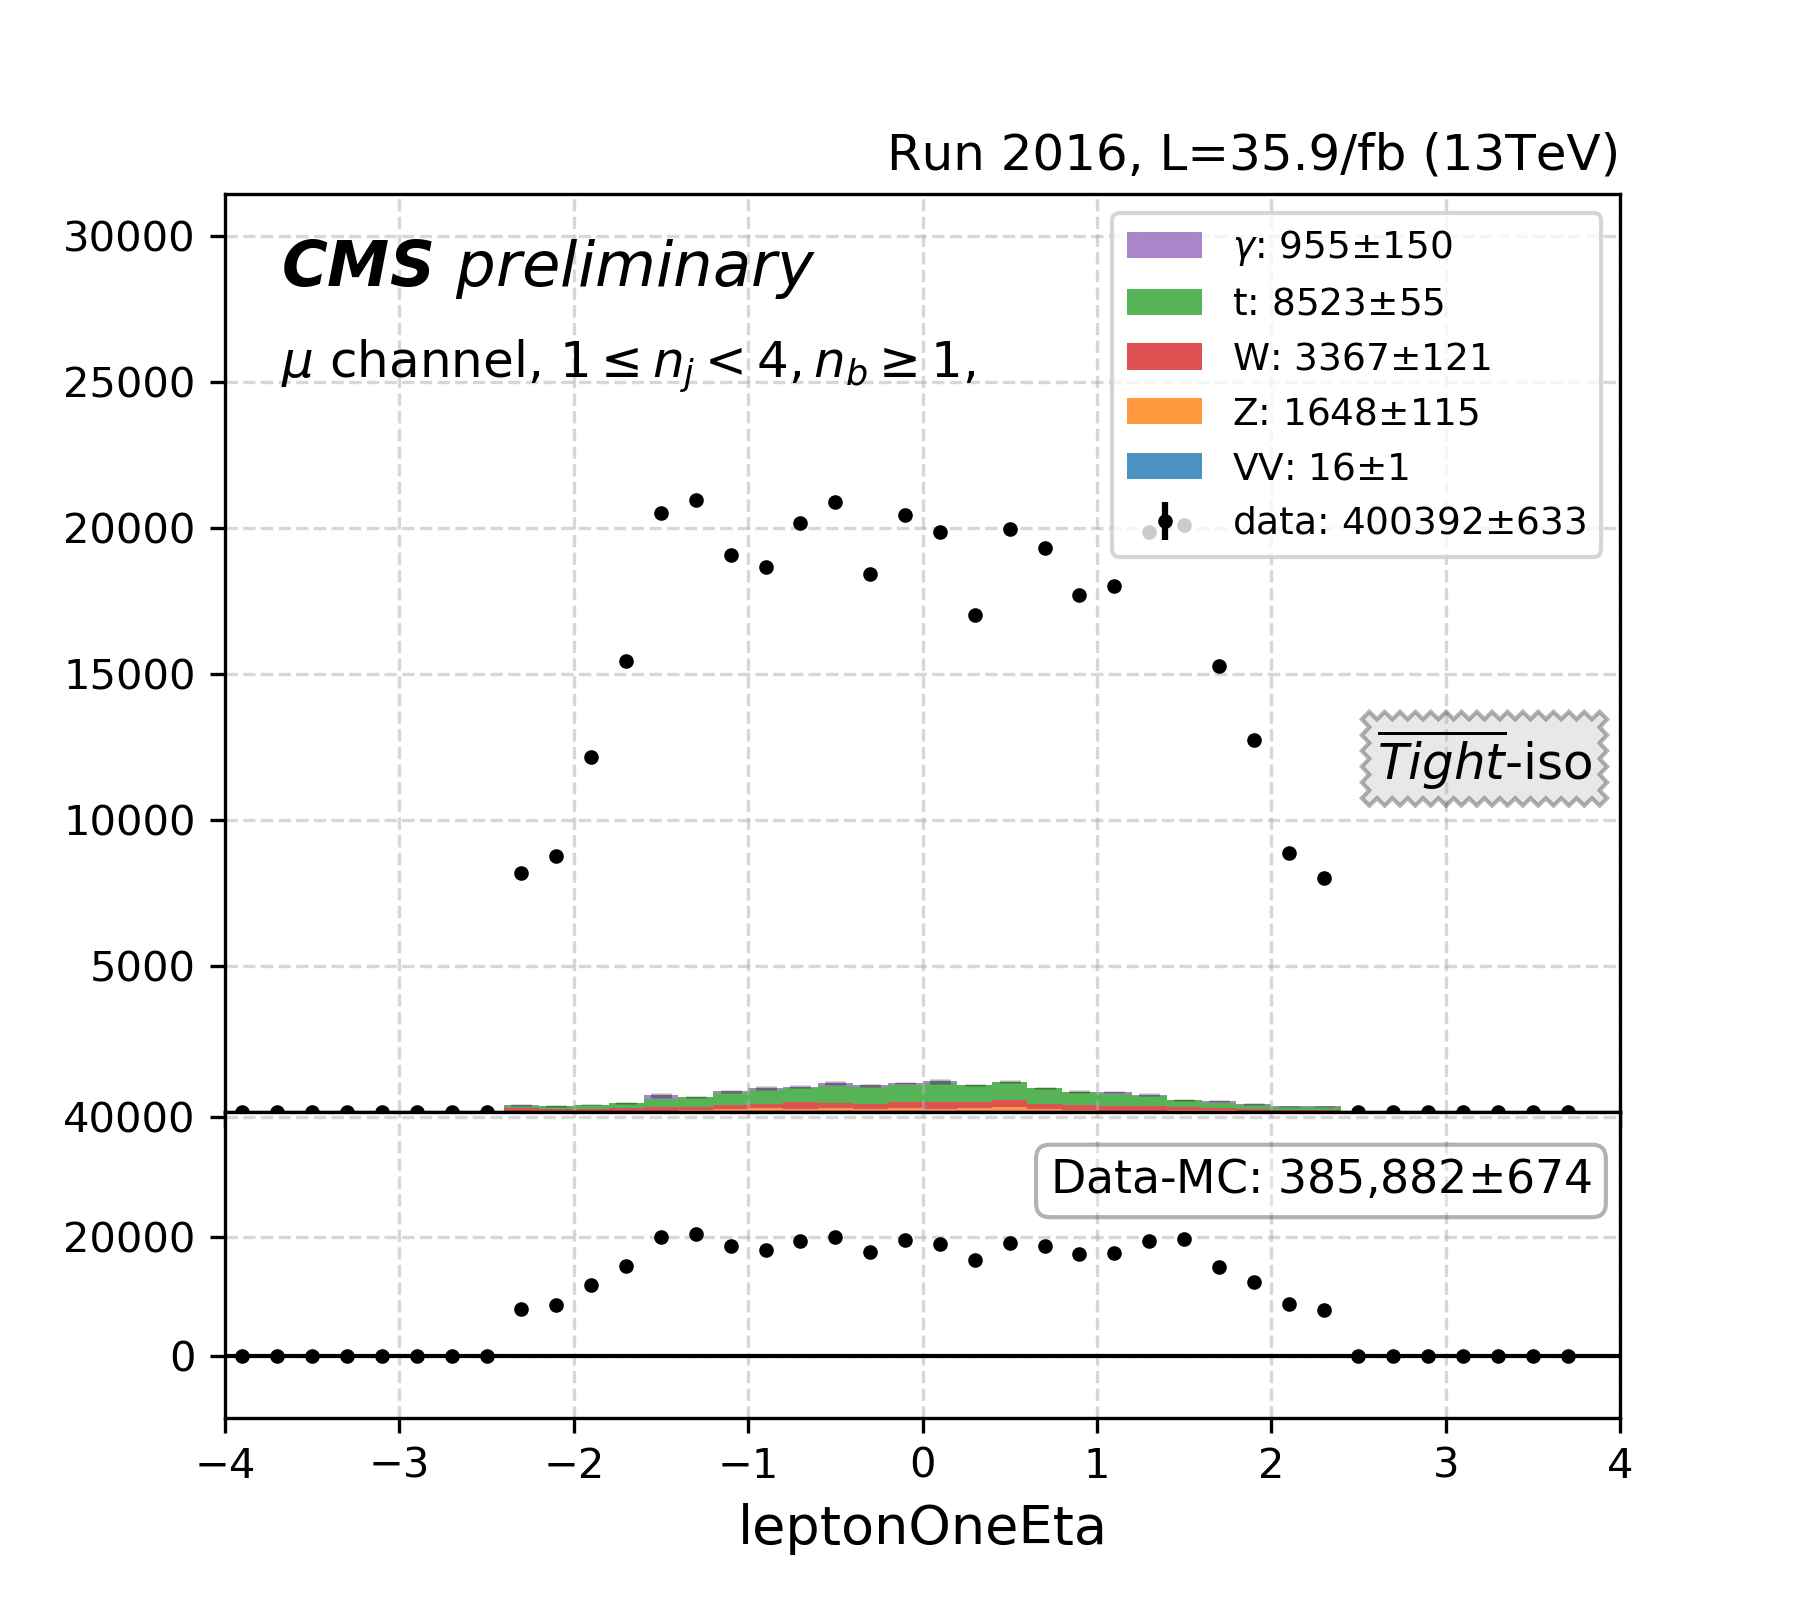
\includegraphics[width=0.24\textwidth]{chapters/Appendix/sectionQCD/figures/123j1b/mu_leptonOneEta_False.png}
    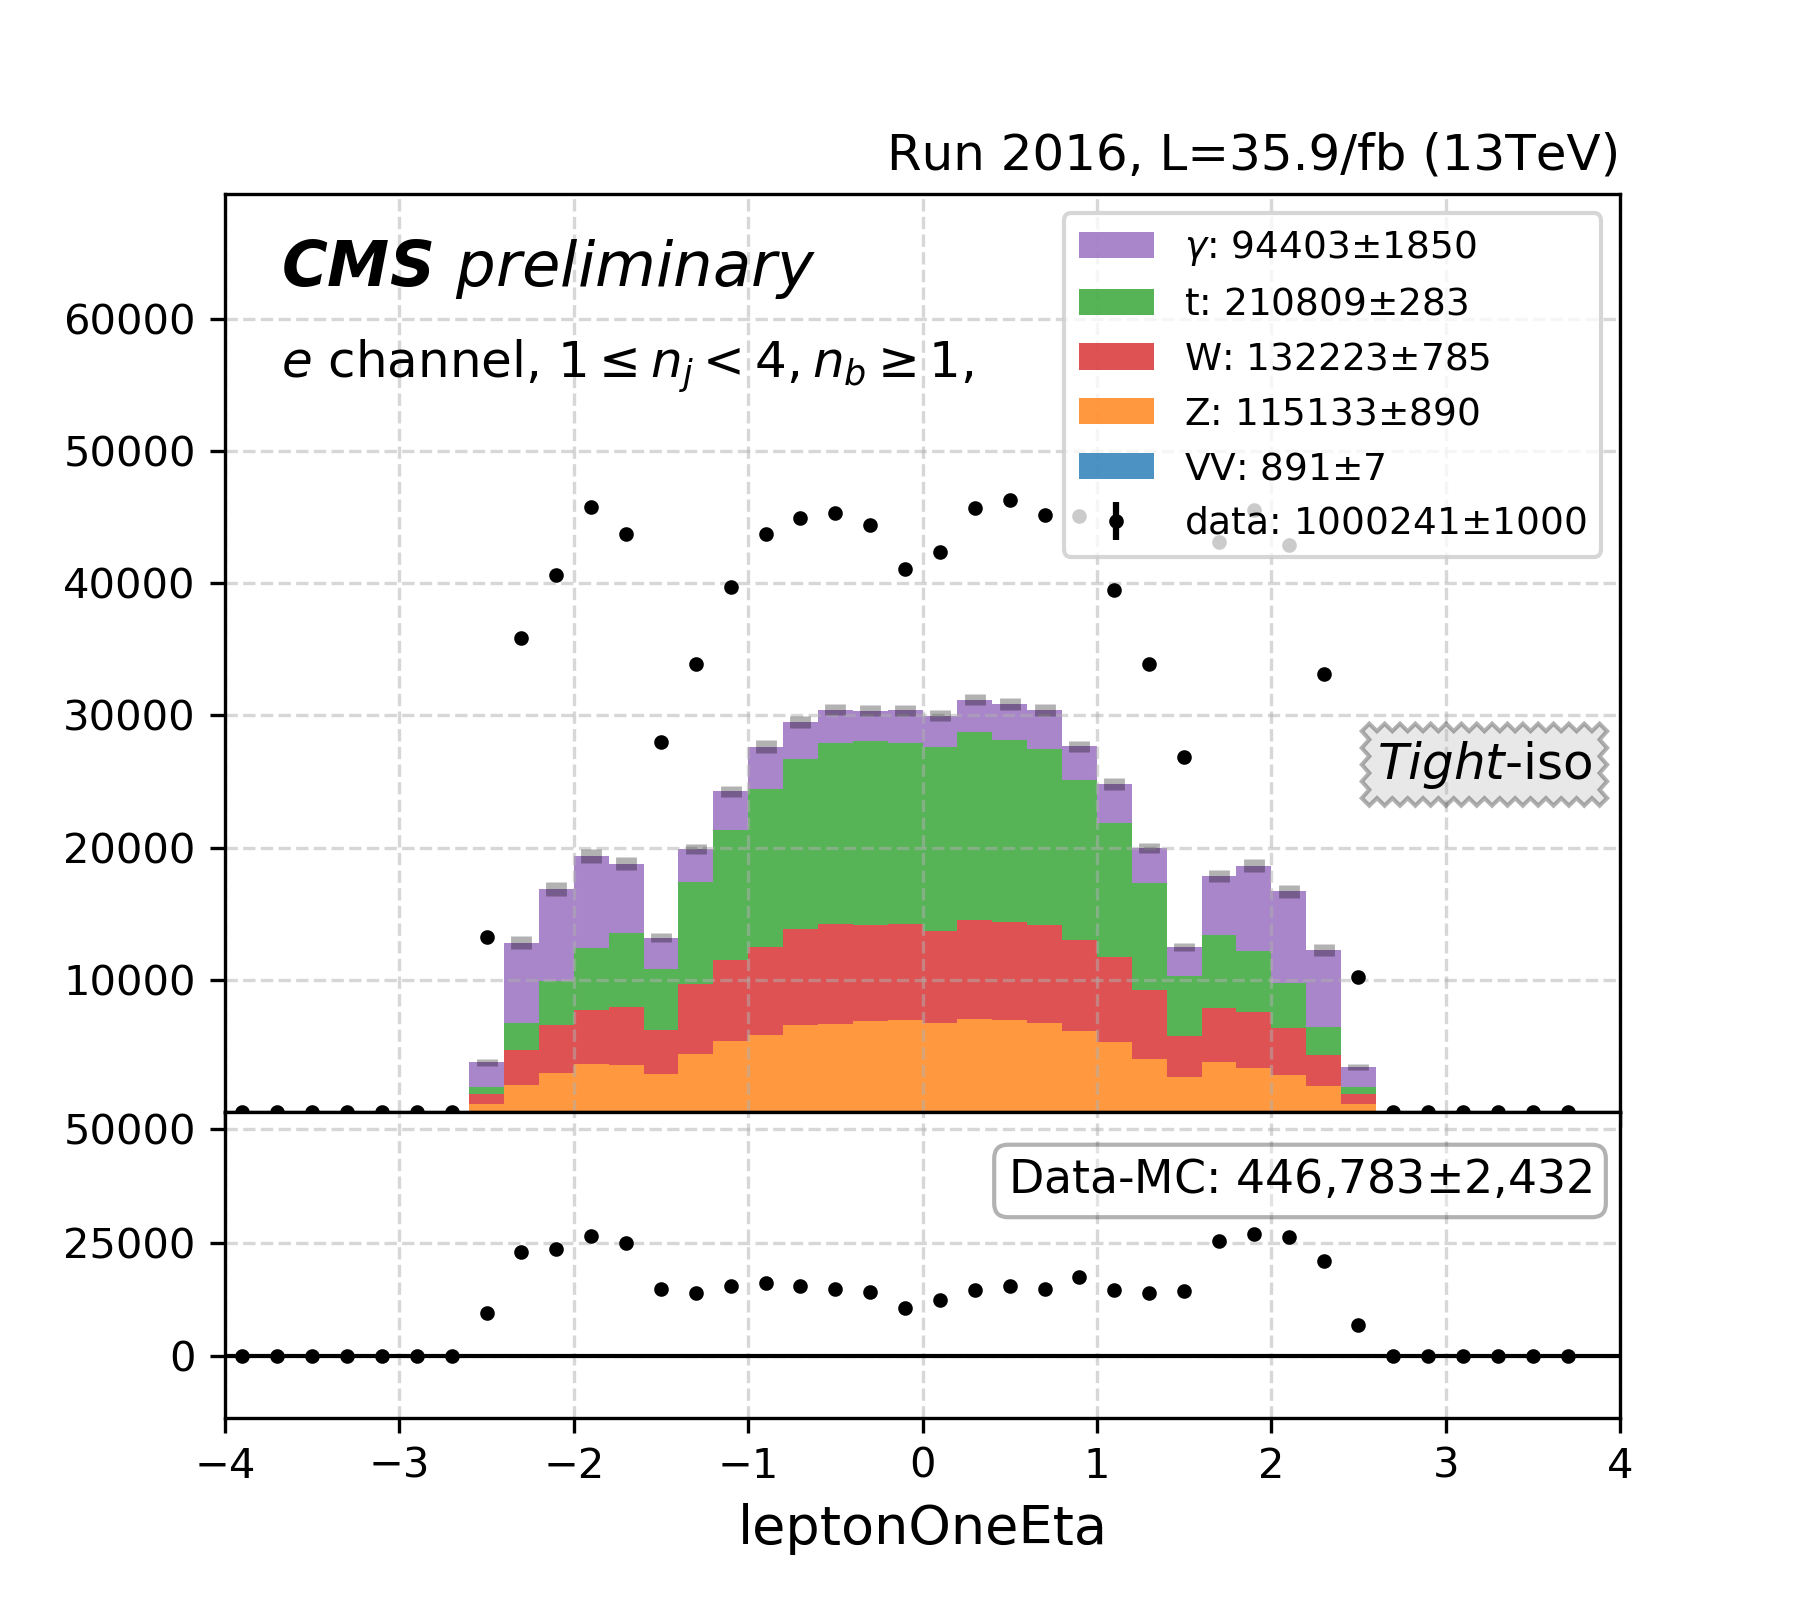
\includegraphics[width=0.24\textwidth]{chapters/Appendix/sectionQCD/figures/123j1b/e_leptonOneEta_True.png}
    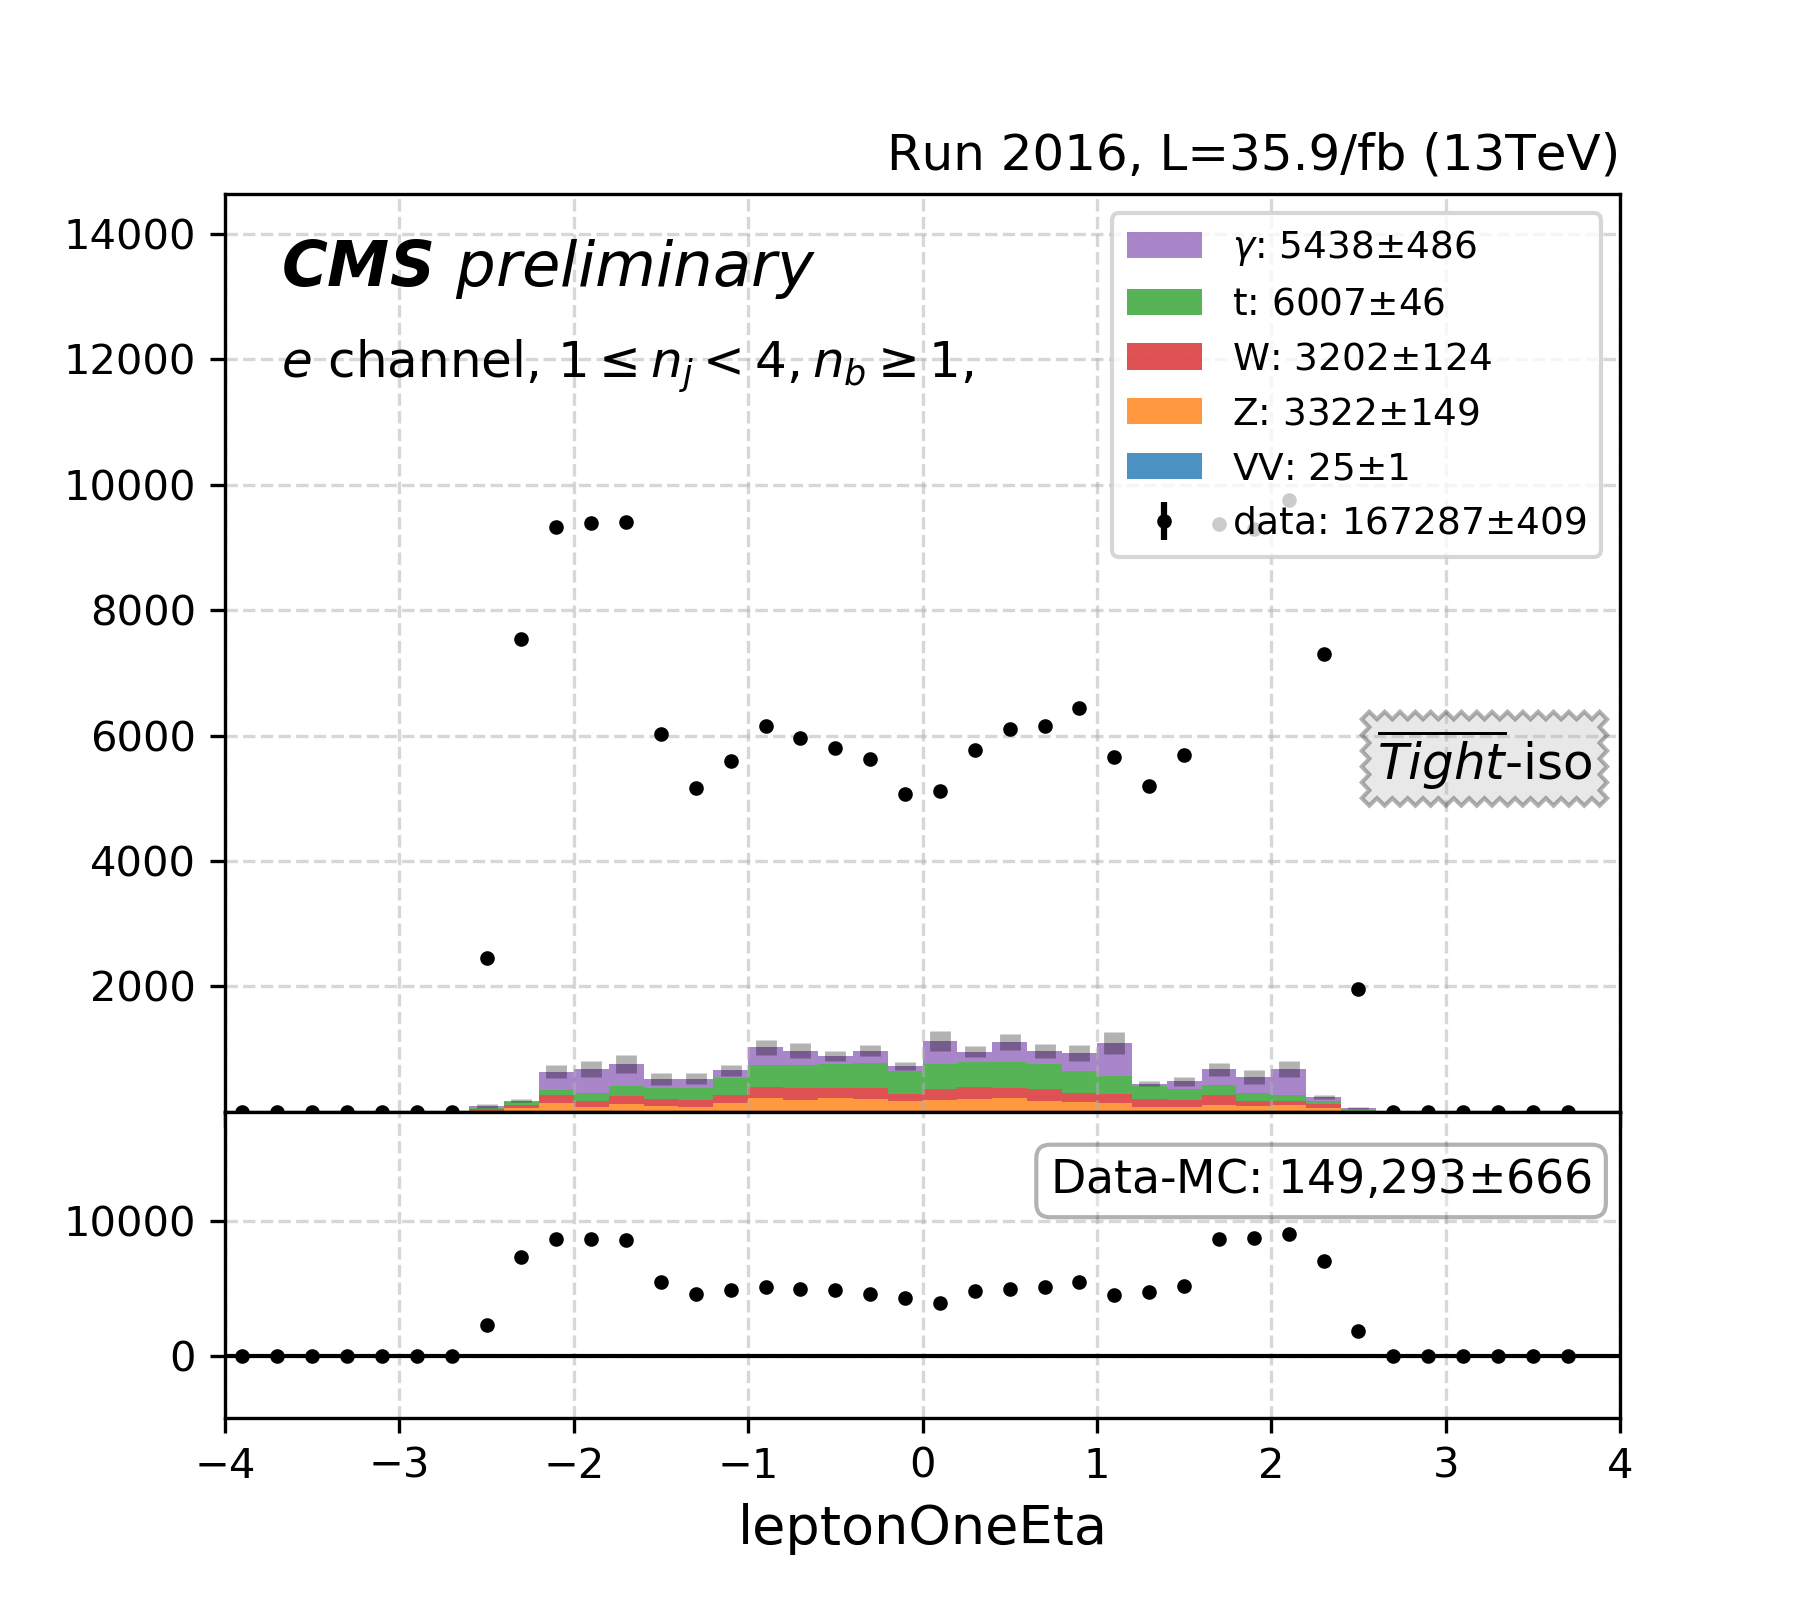
\includegraphics[width=0.24\textwidth]{chapters/Appendix/sectionQCD/figures/123j1b/e_leptonOneEta_False.png}
    
    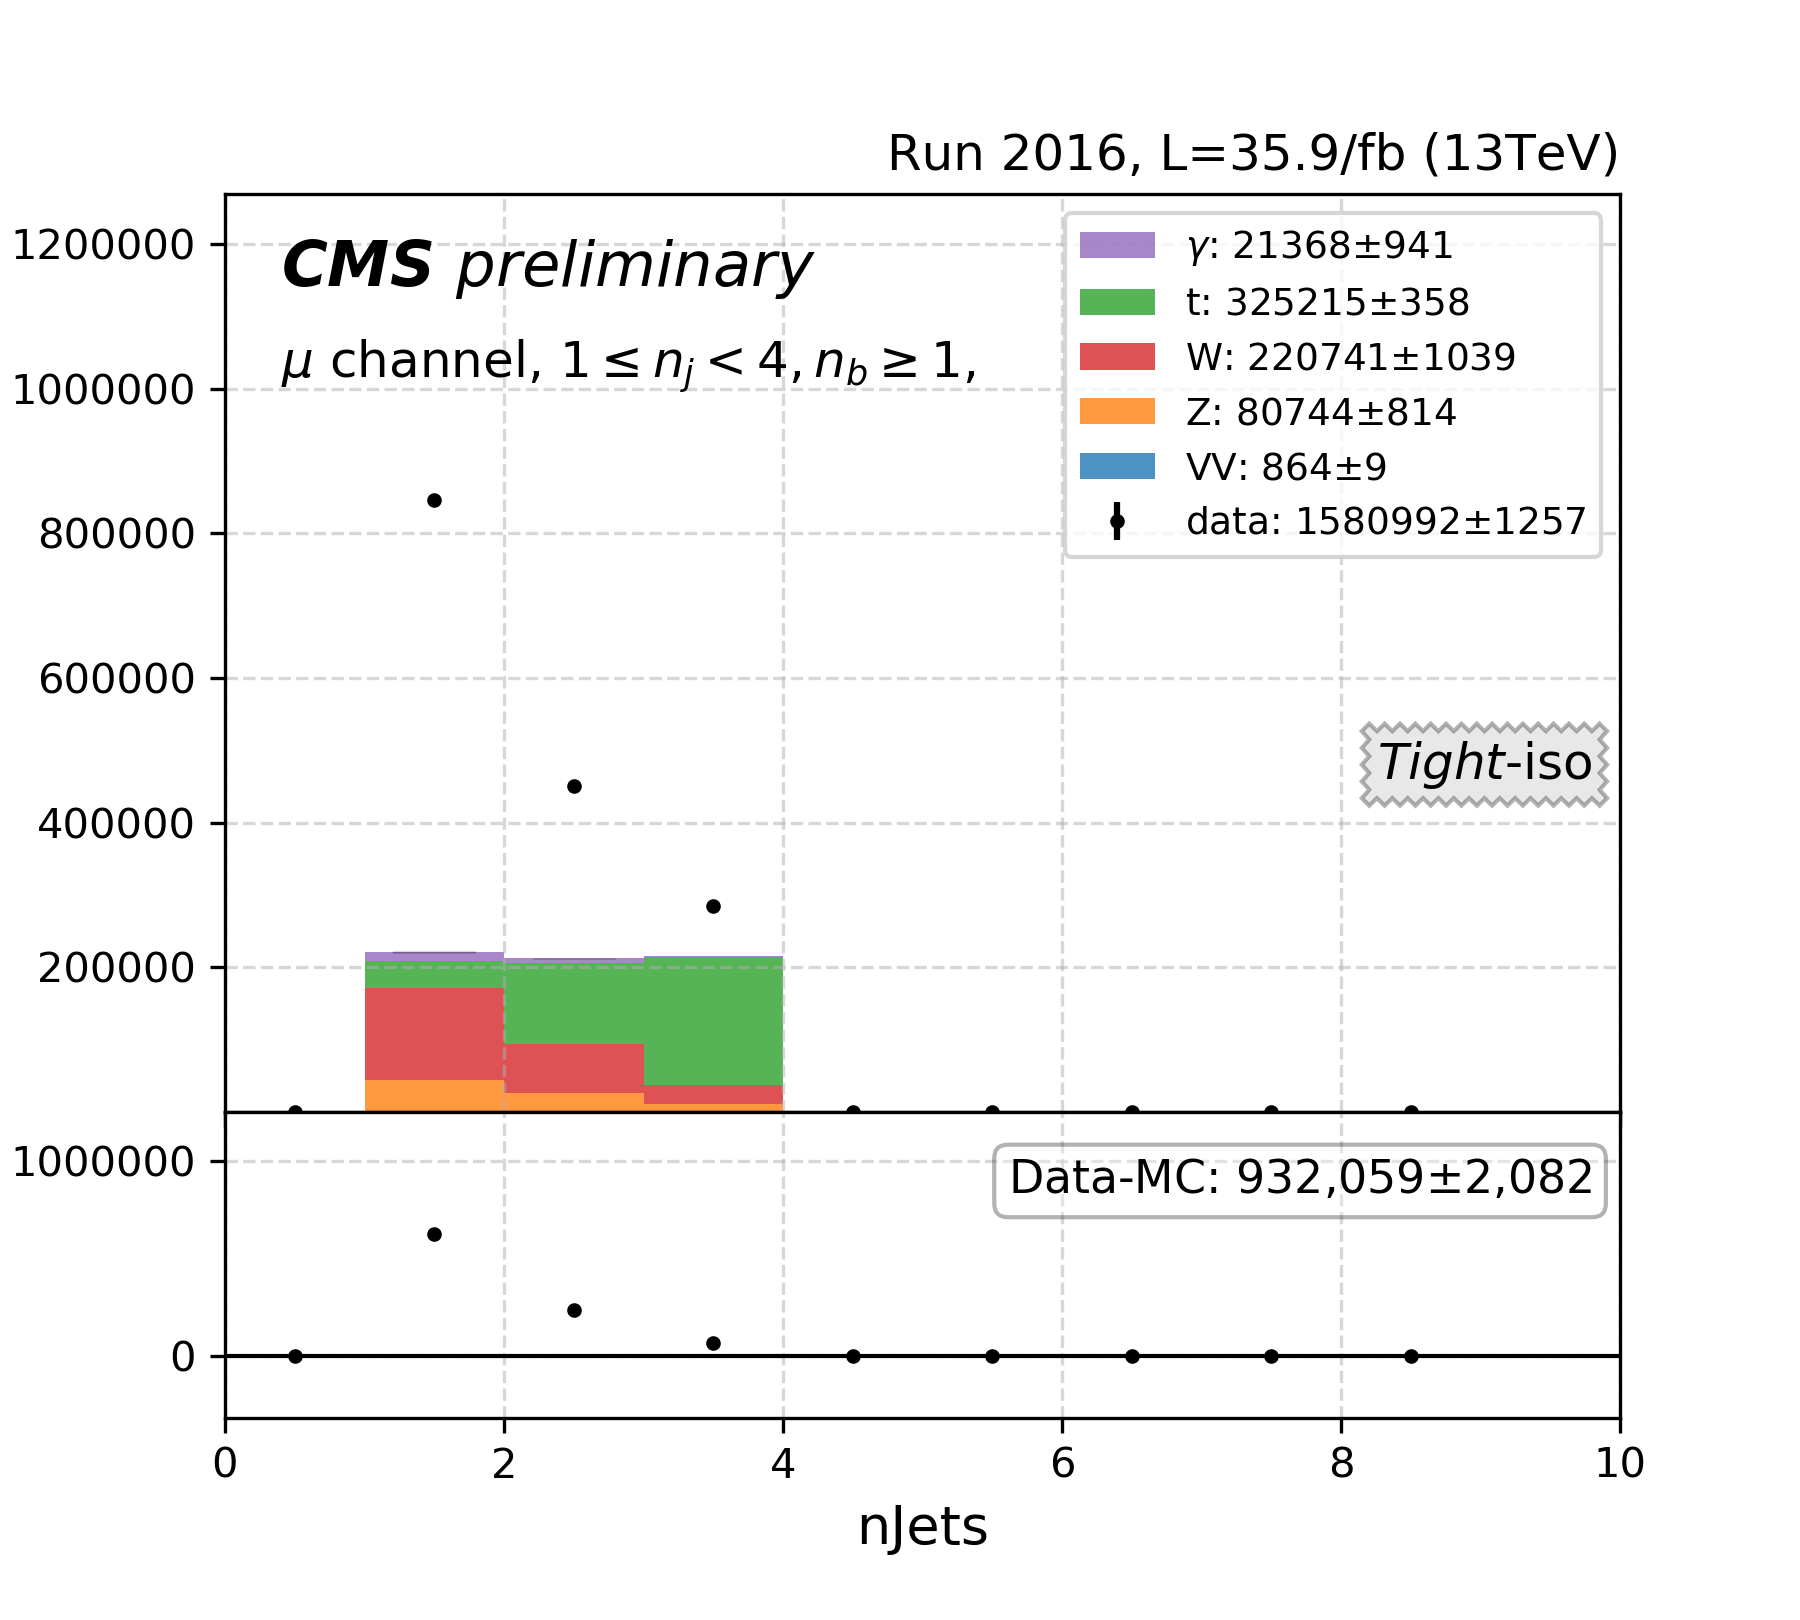
\includegraphics[width=0.24\textwidth]{chapters/Appendix/sectionQCD/figures/123j1b/mu_nJets_True.png}
    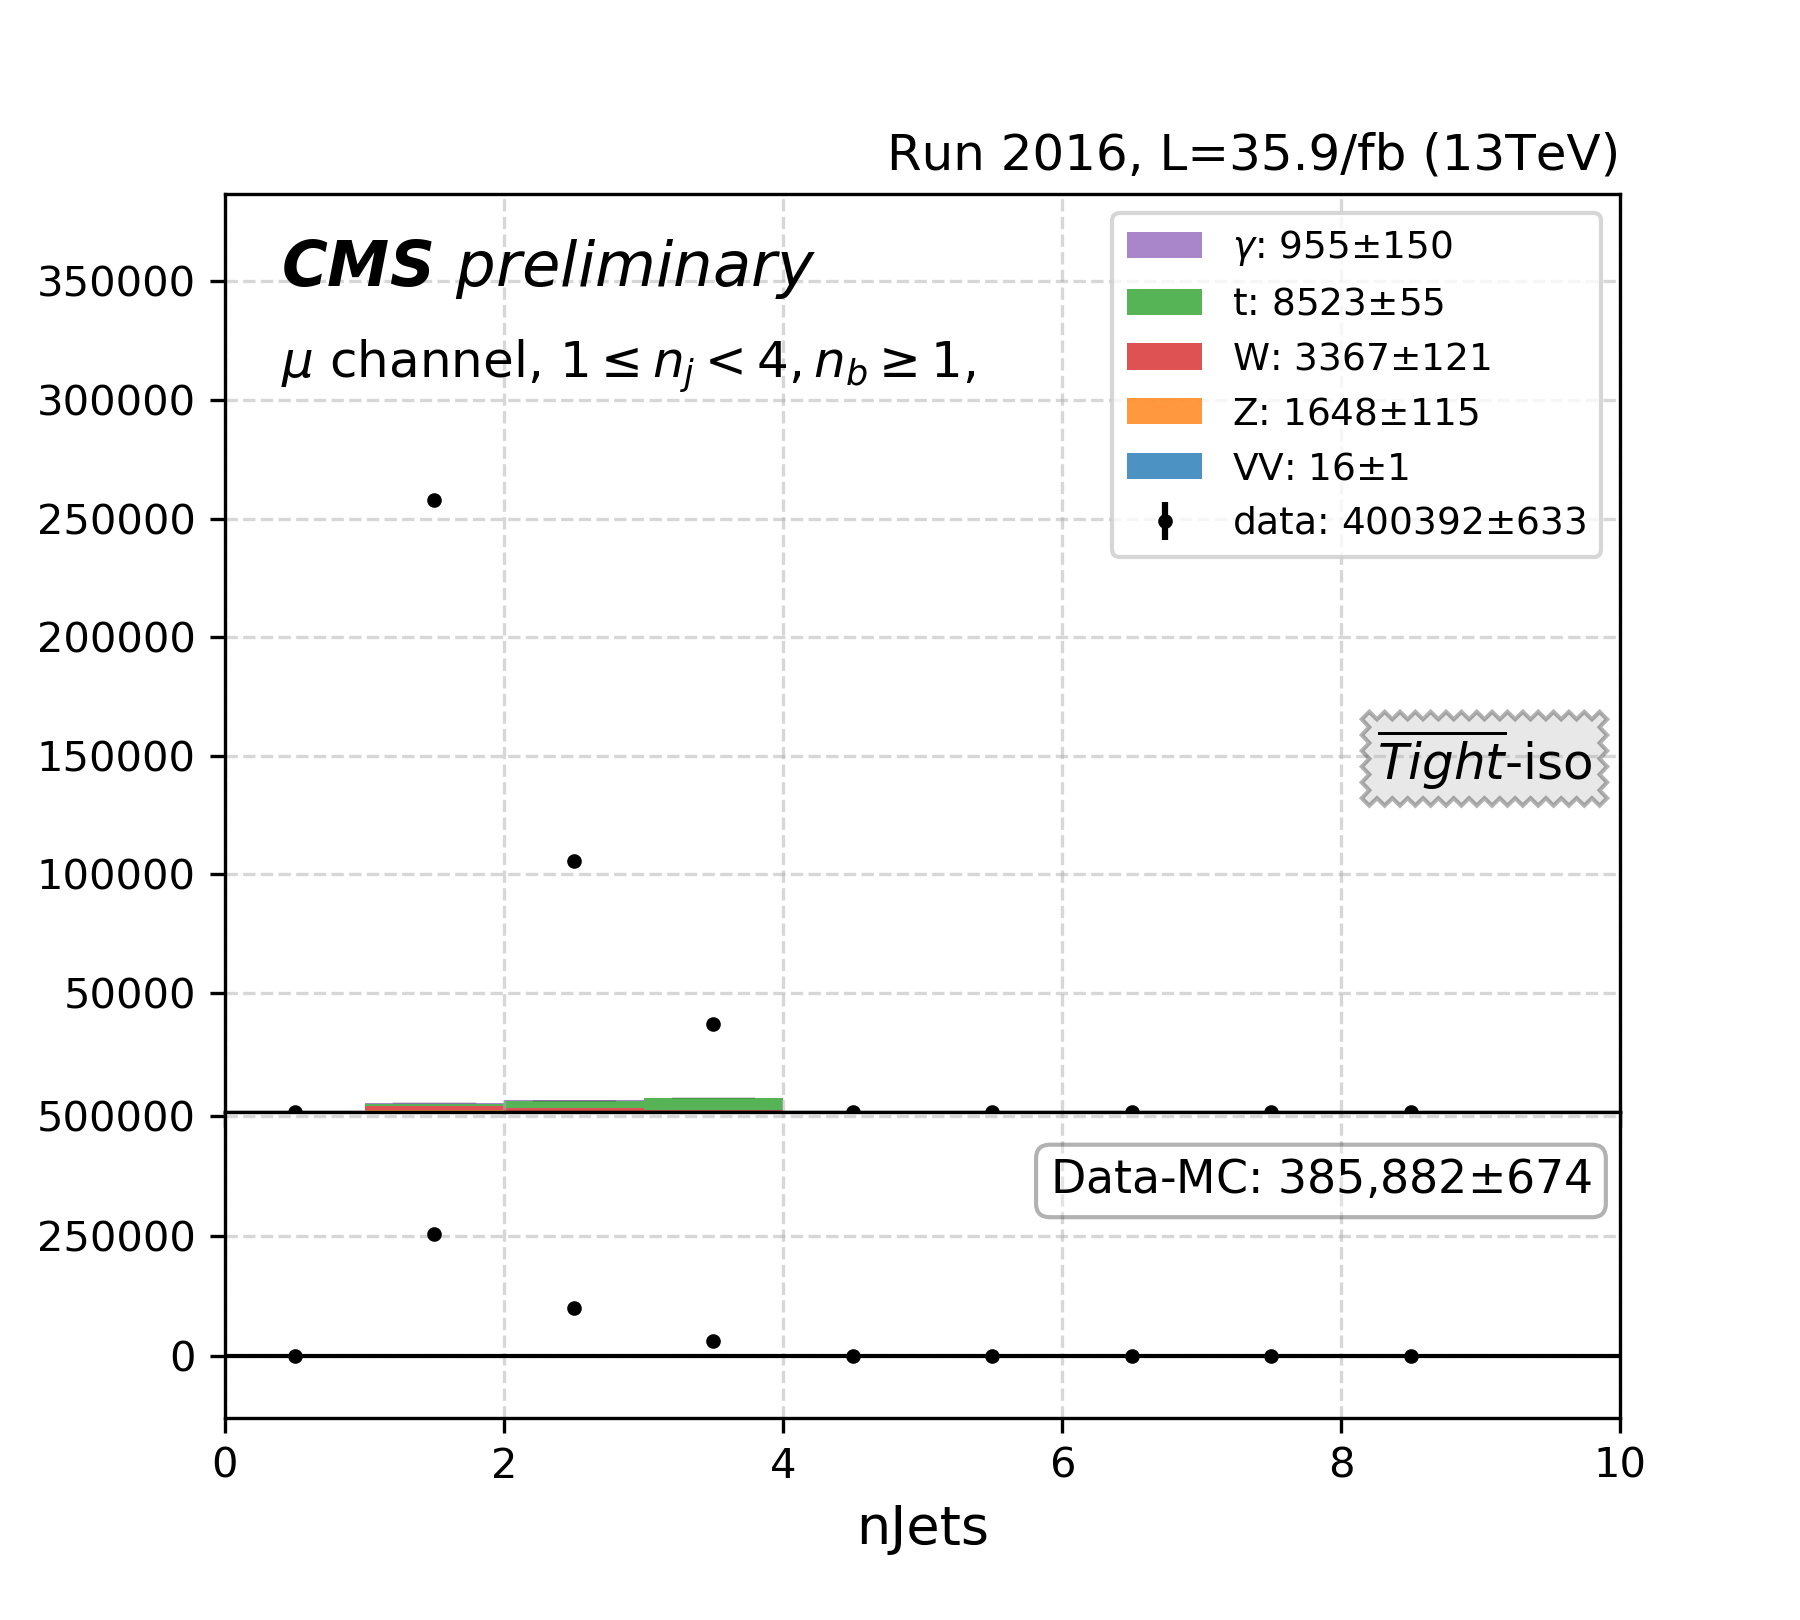
\includegraphics[width=0.24\textwidth]{chapters/Appendix/sectionQCD/figures/123j1b/mu_nJets_False.png}
    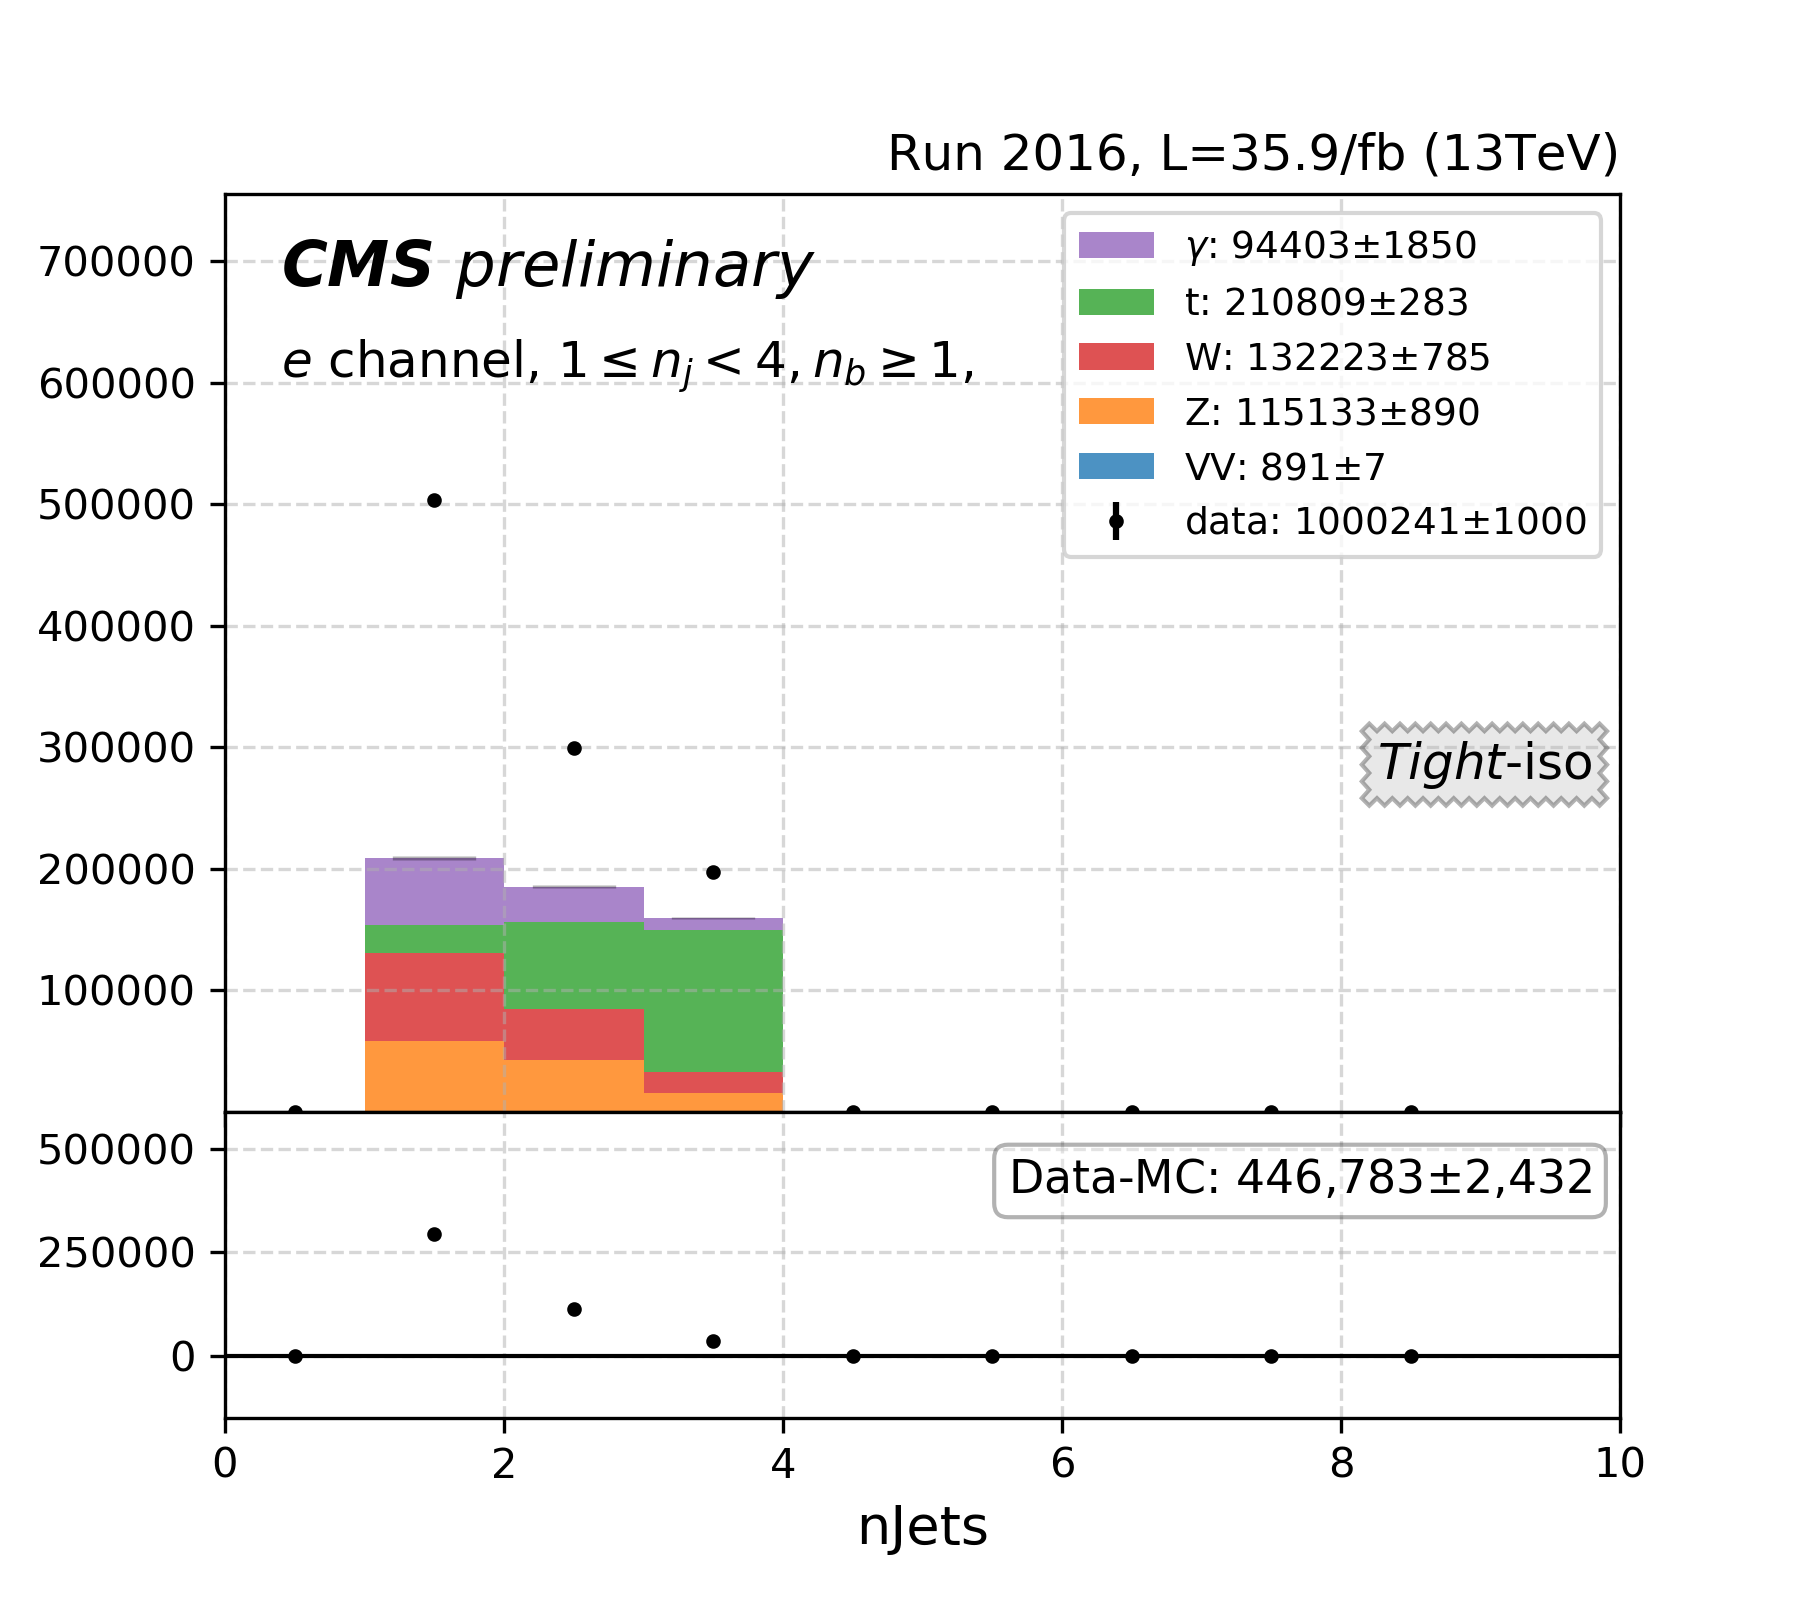
\includegraphics[width=0.24\textwidth]{chapters/Appendix/sectionQCD/figures/123j1b/e_nJets_True.png}
    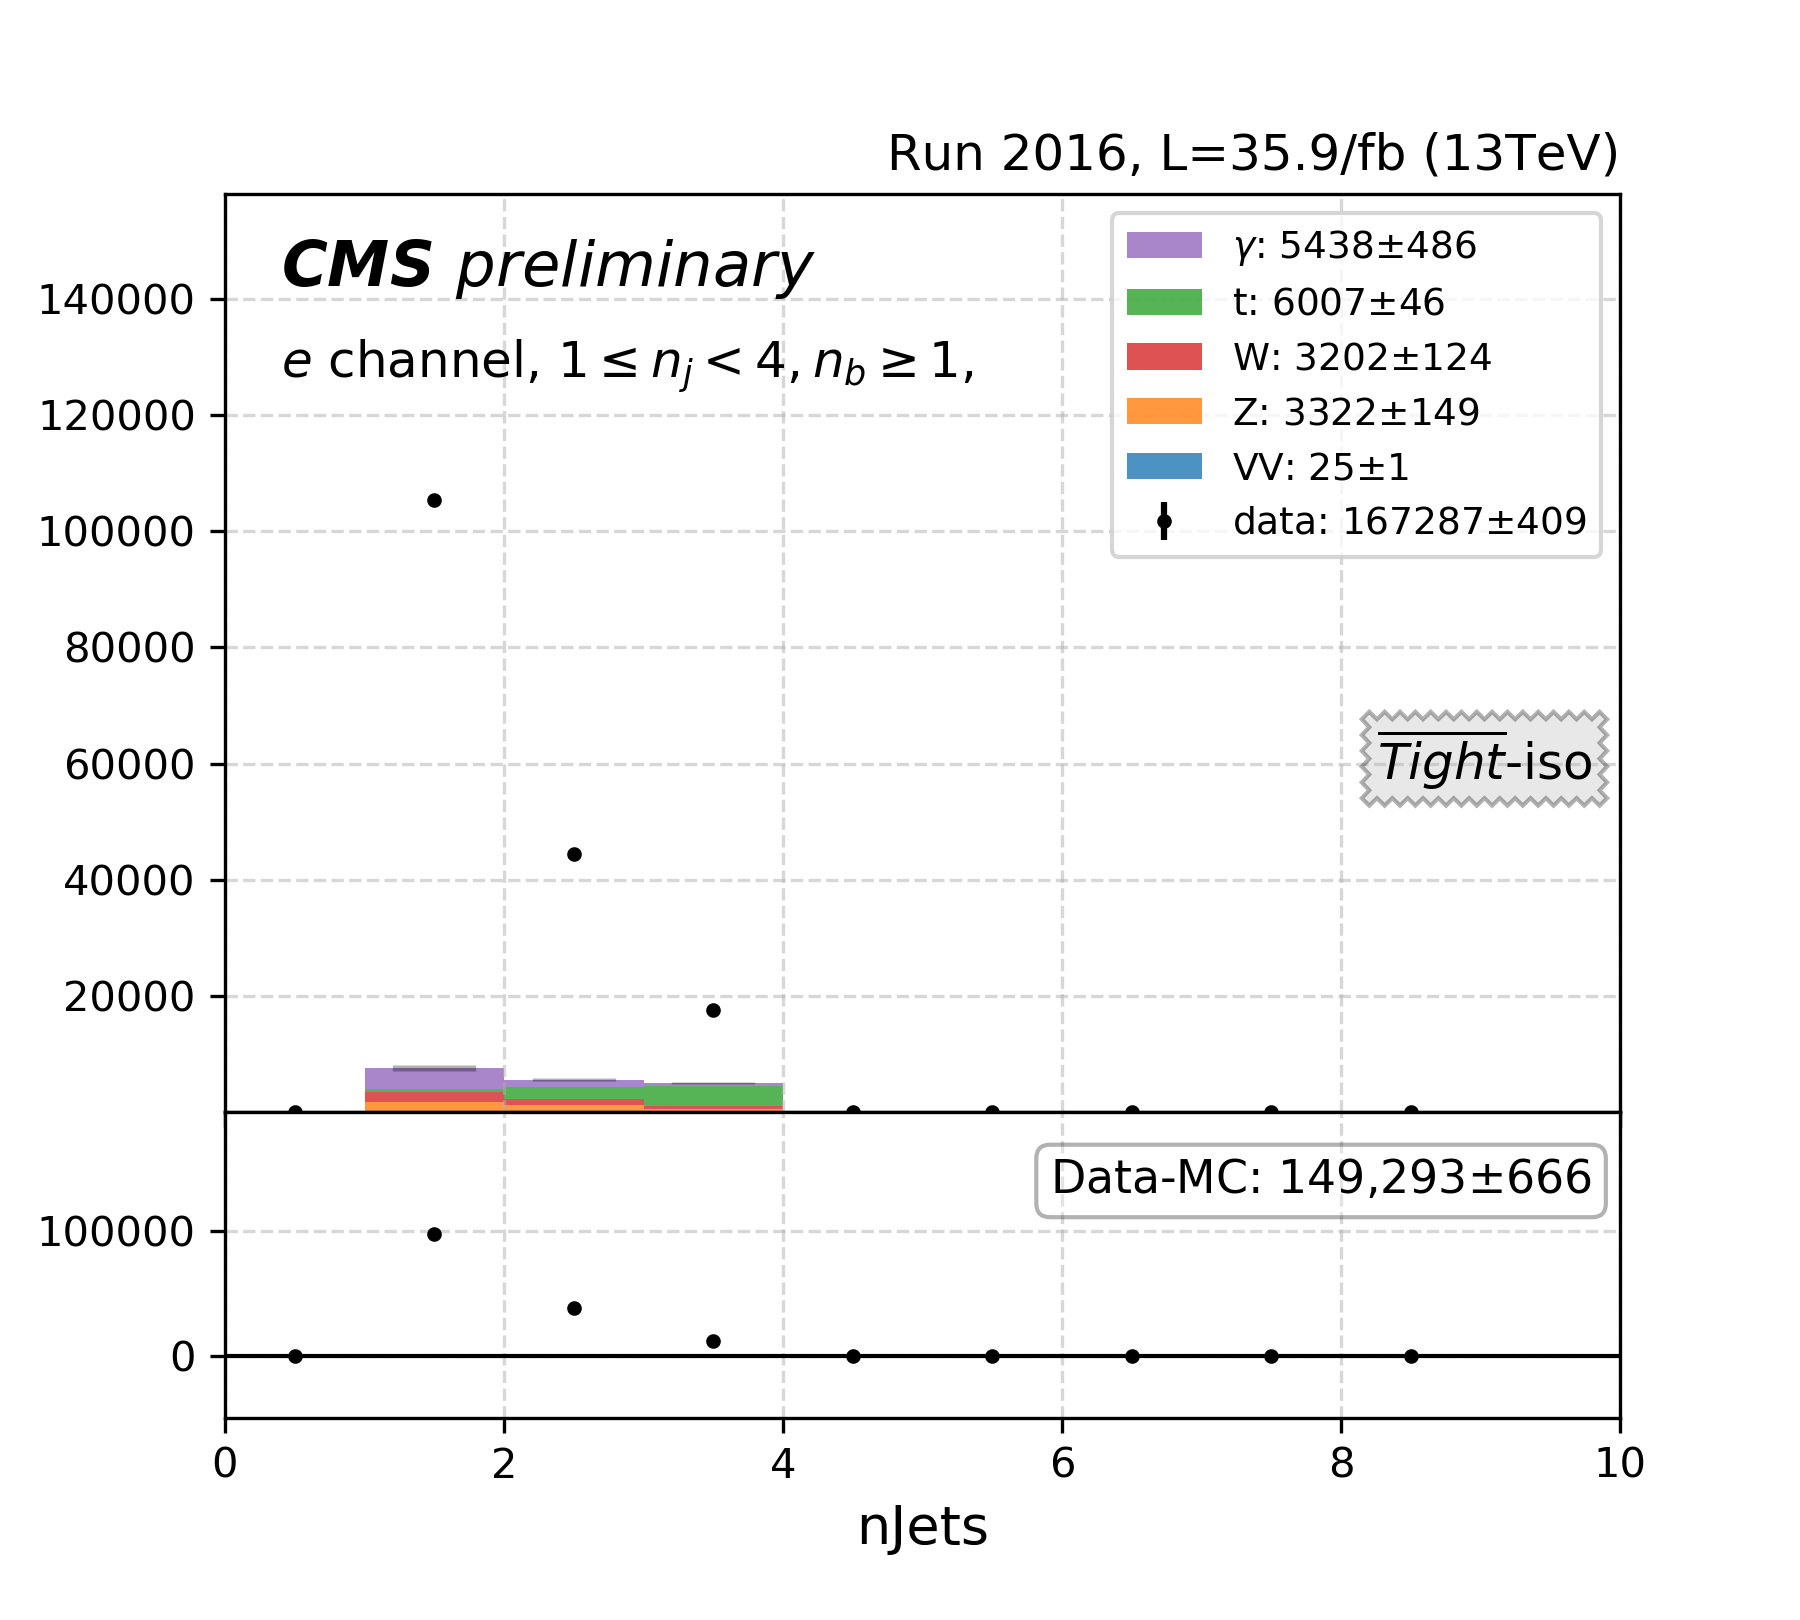
\includegraphics[width=0.24\textwidth]{chapters/Appendix/sectionQCD/figures/123j1b/e_nJets_False.png}
    
    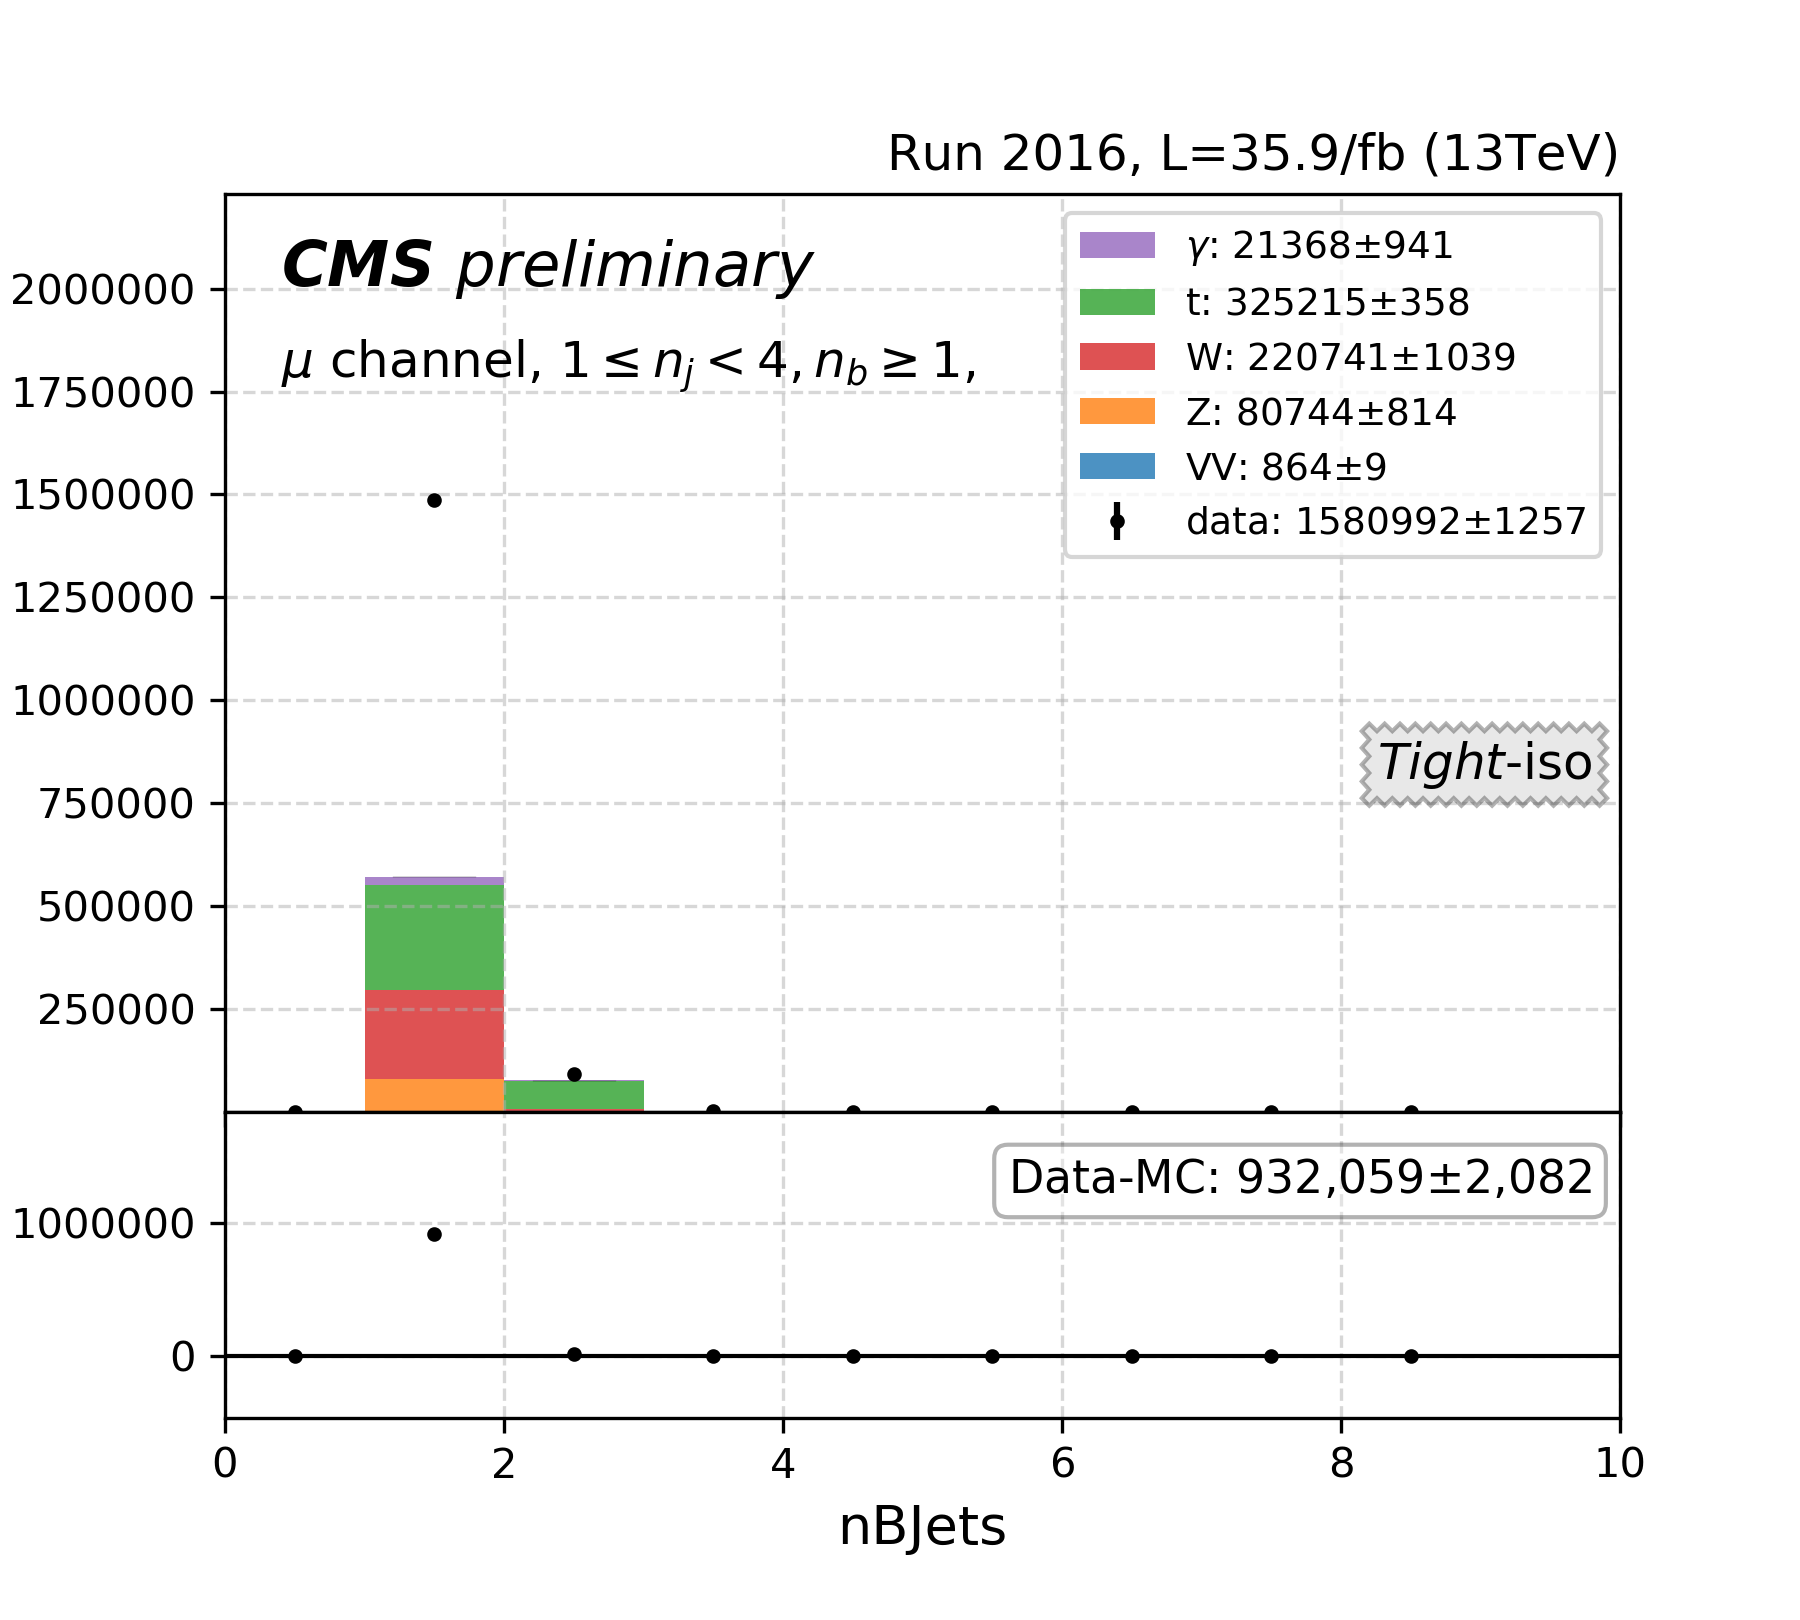
\includegraphics[width=0.24\textwidth]{chapters/Appendix/sectionQCD/figures/123j1b/mu_nBJets_True.png}
    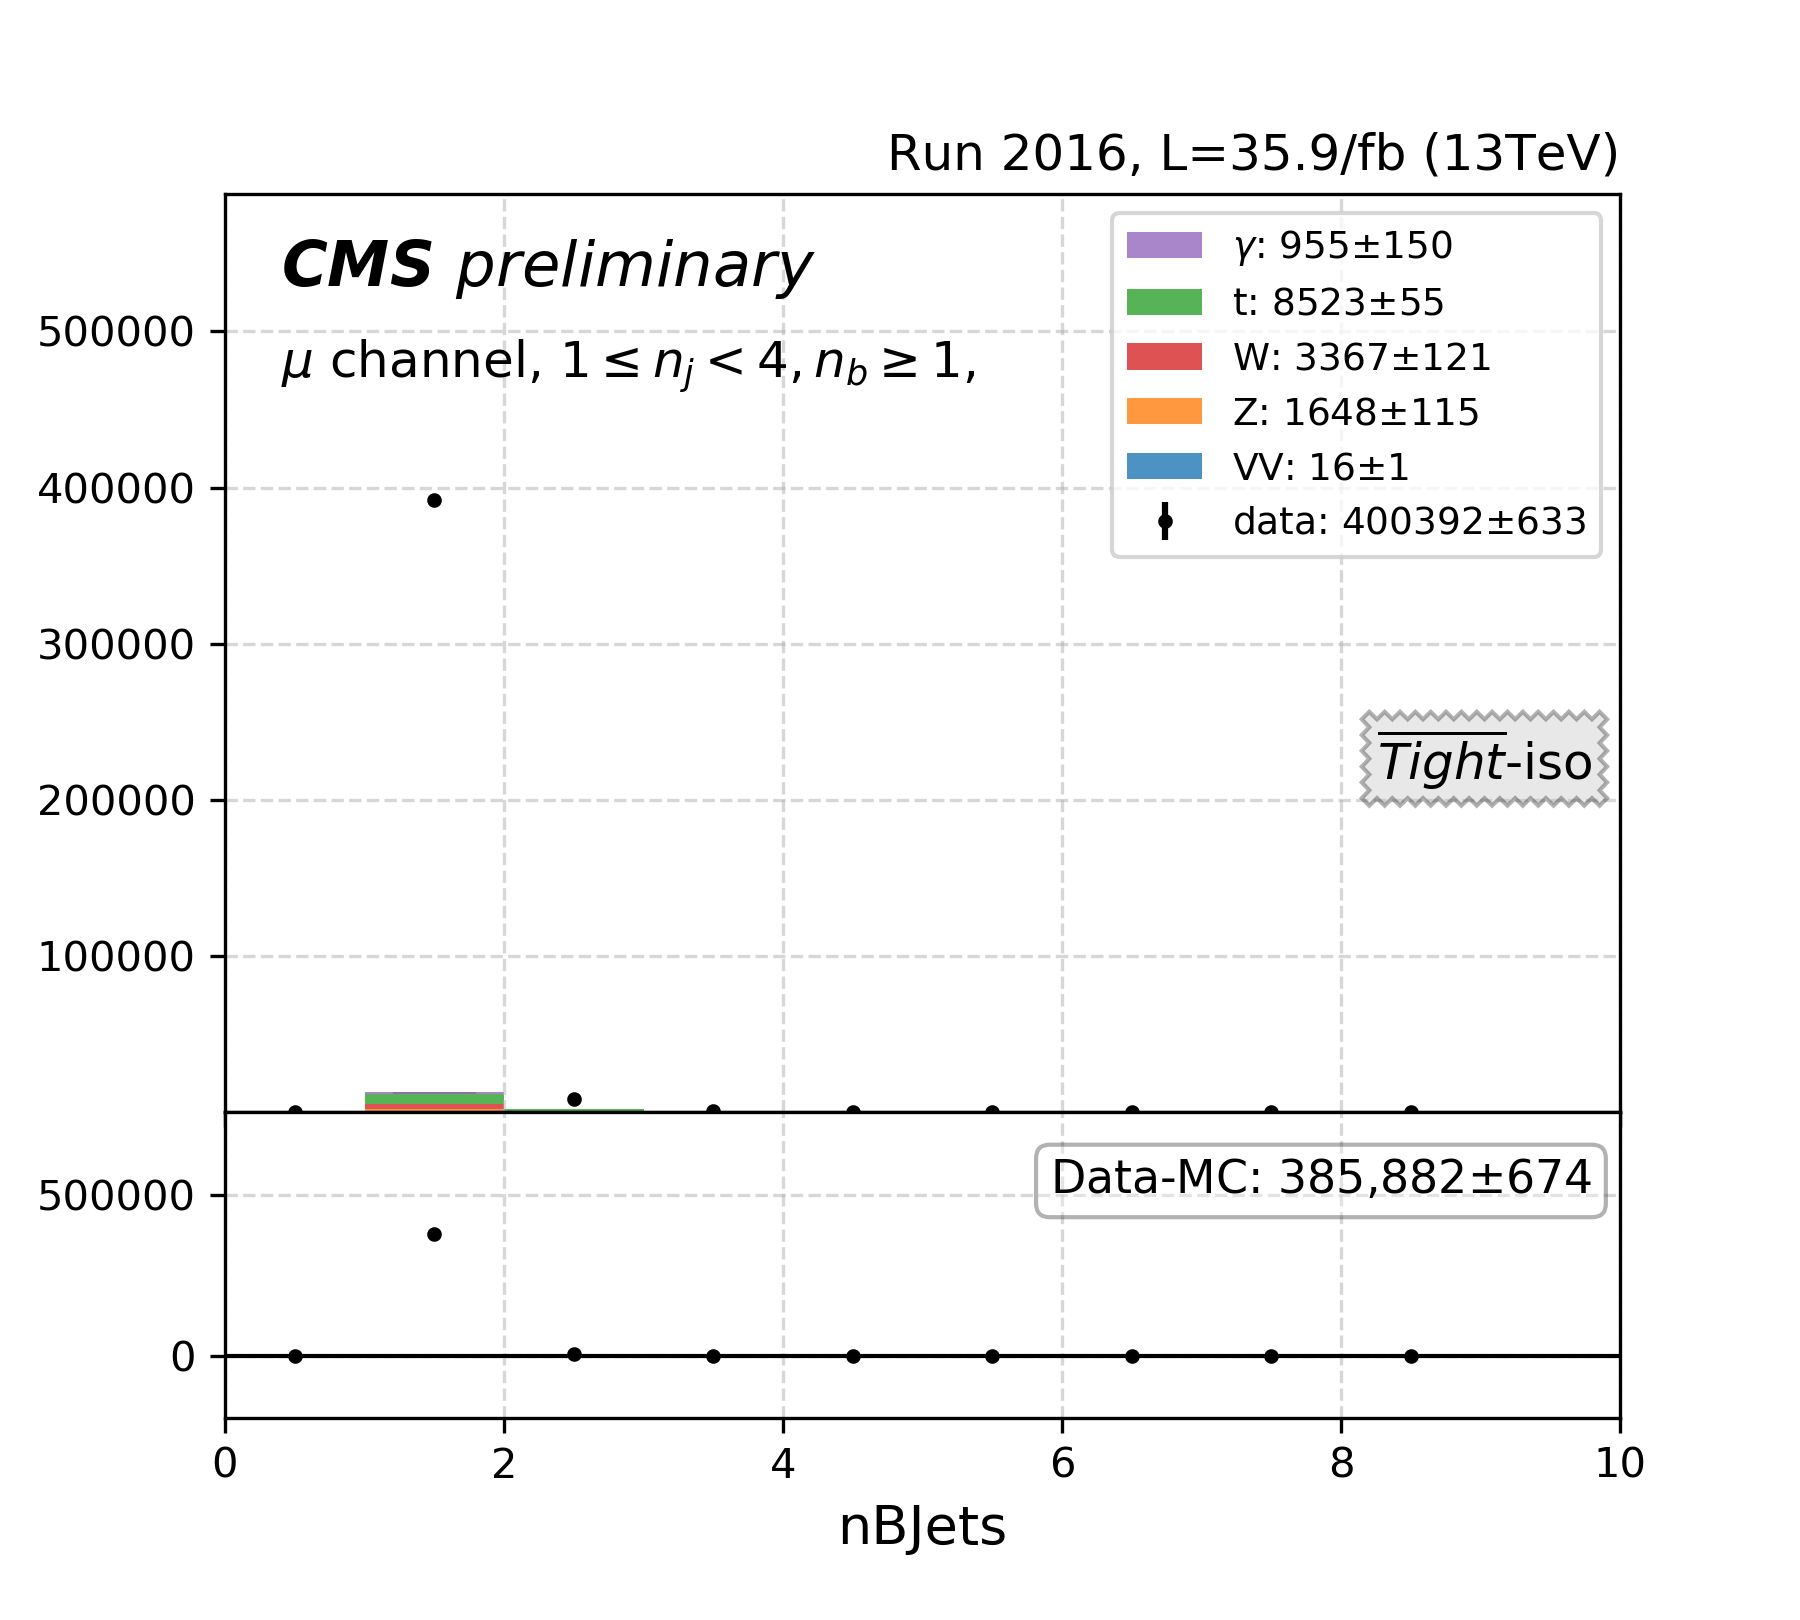
\includegraphics[width=0.24\textwidth]{chapters/Appendix/sectionQCD/figures/123j1b/mu_nBJets_False.png}
    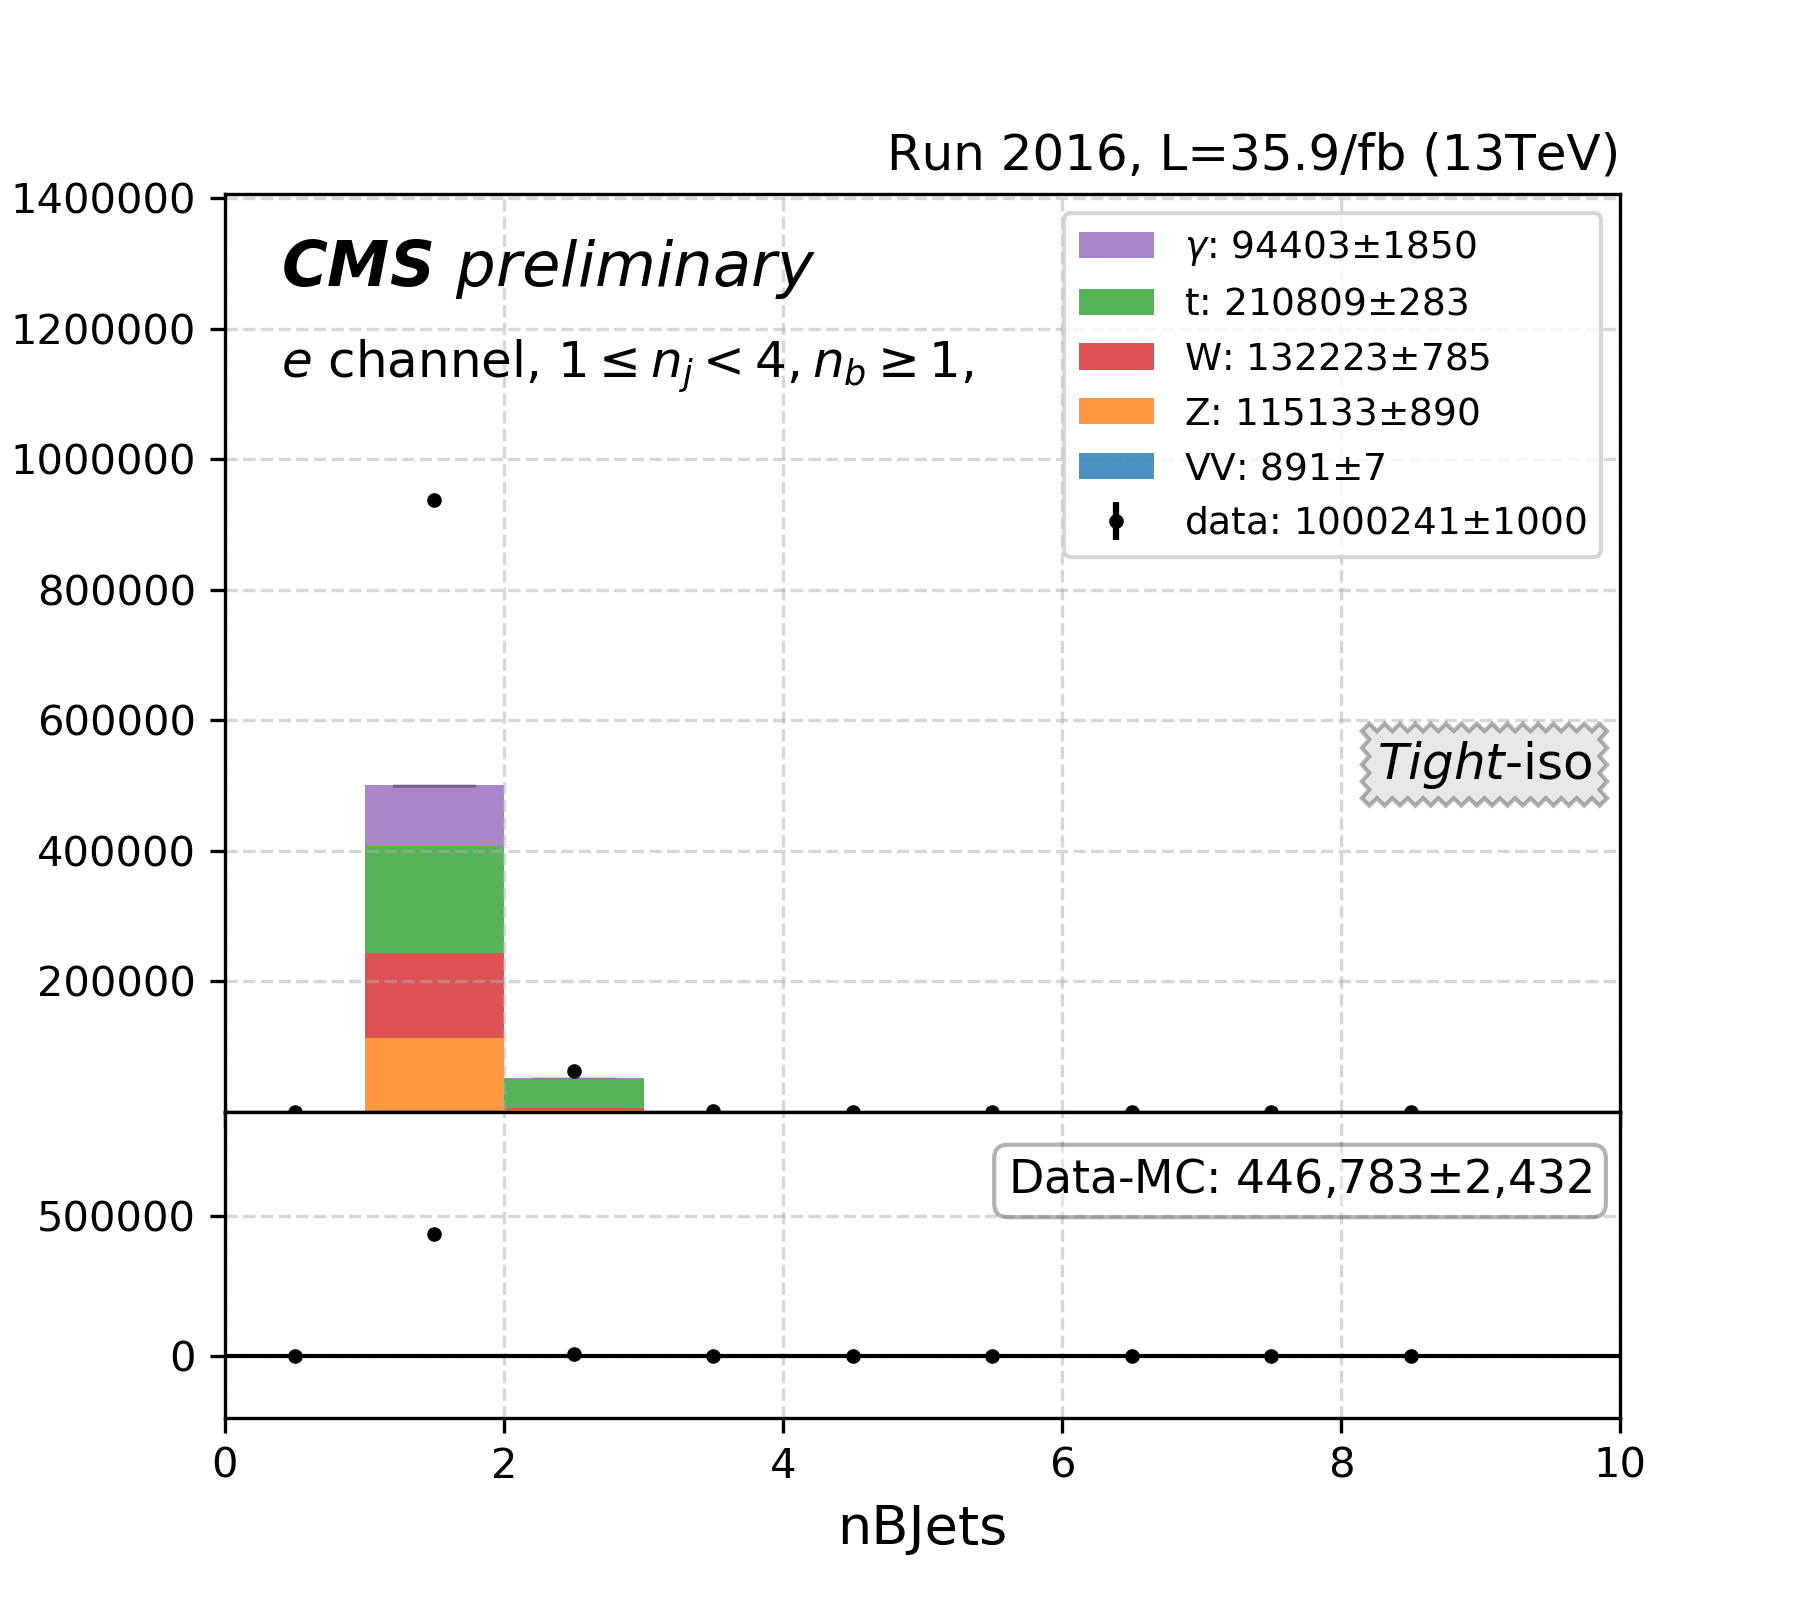
\includegraphics[width=0.24\textwidth]{chapters/Appendix/sectionQCD/figures/123j1b/e_nBJets_True.png}
    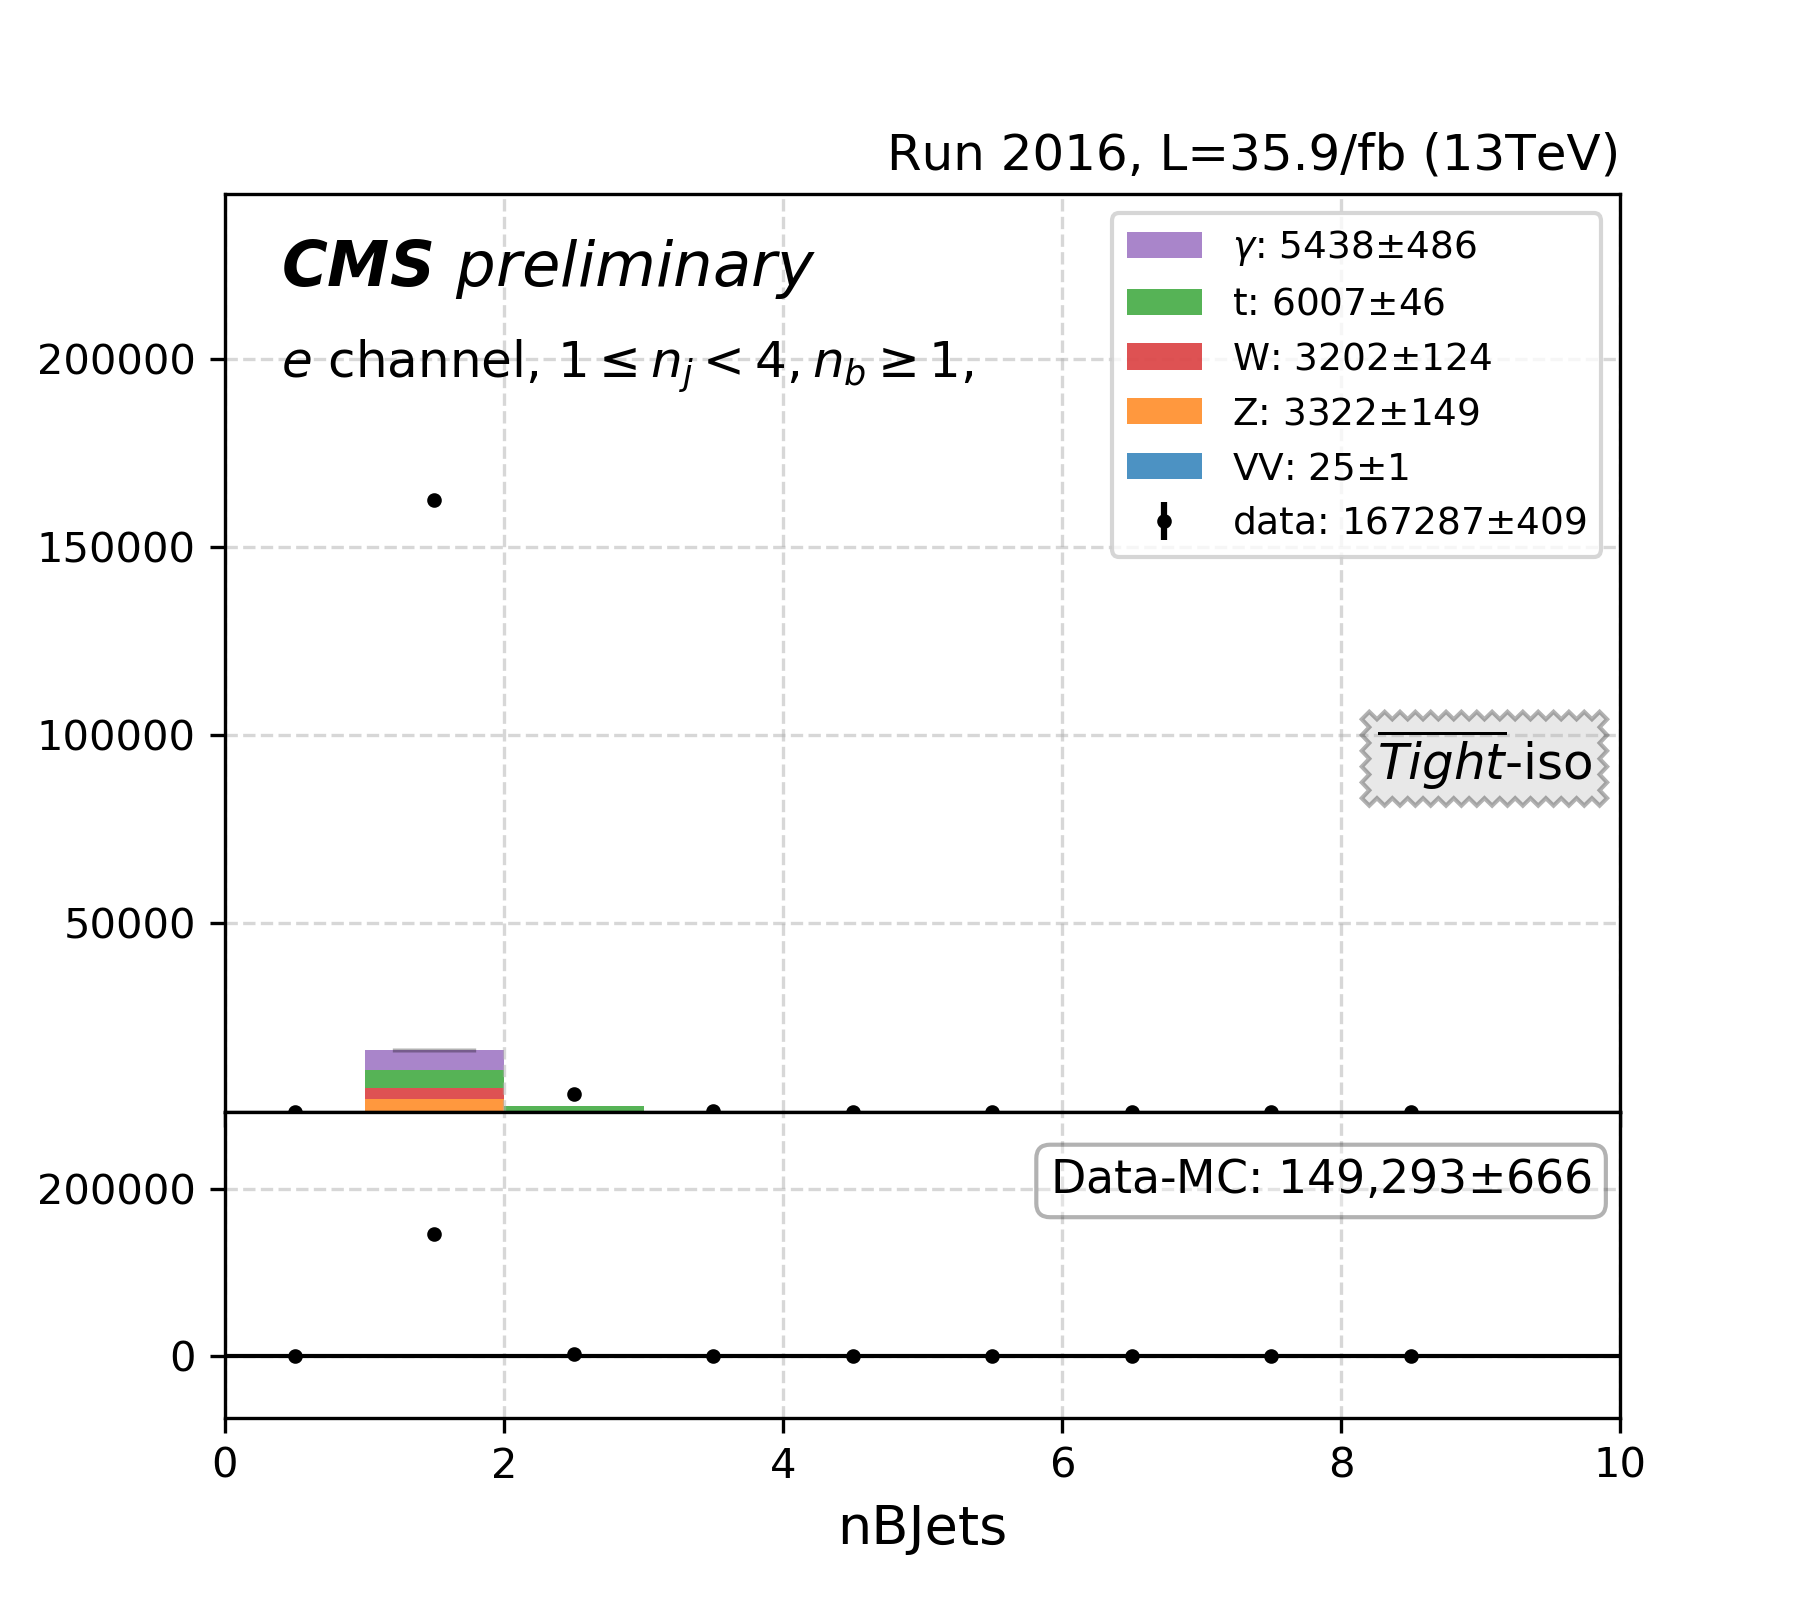
\includegraphics[width=0.24\textwidth]{chapters/Appendix/sectionQCD/figures/123j1b/e_nBJets_False.png}
    

    \caption{The iso and anti-iso region of $\mu$+jet (left two columns) and $e$+jet (right two columns) channel 
    with $1\leq n_j <4, n_b\geq1$, which is orthogonal to the $n_j\geq4,n_b\geq1$ signal region.
    }
    \label{fig:appendix:123j1b}
\end{figure}


\begin{figure}
    \centering
    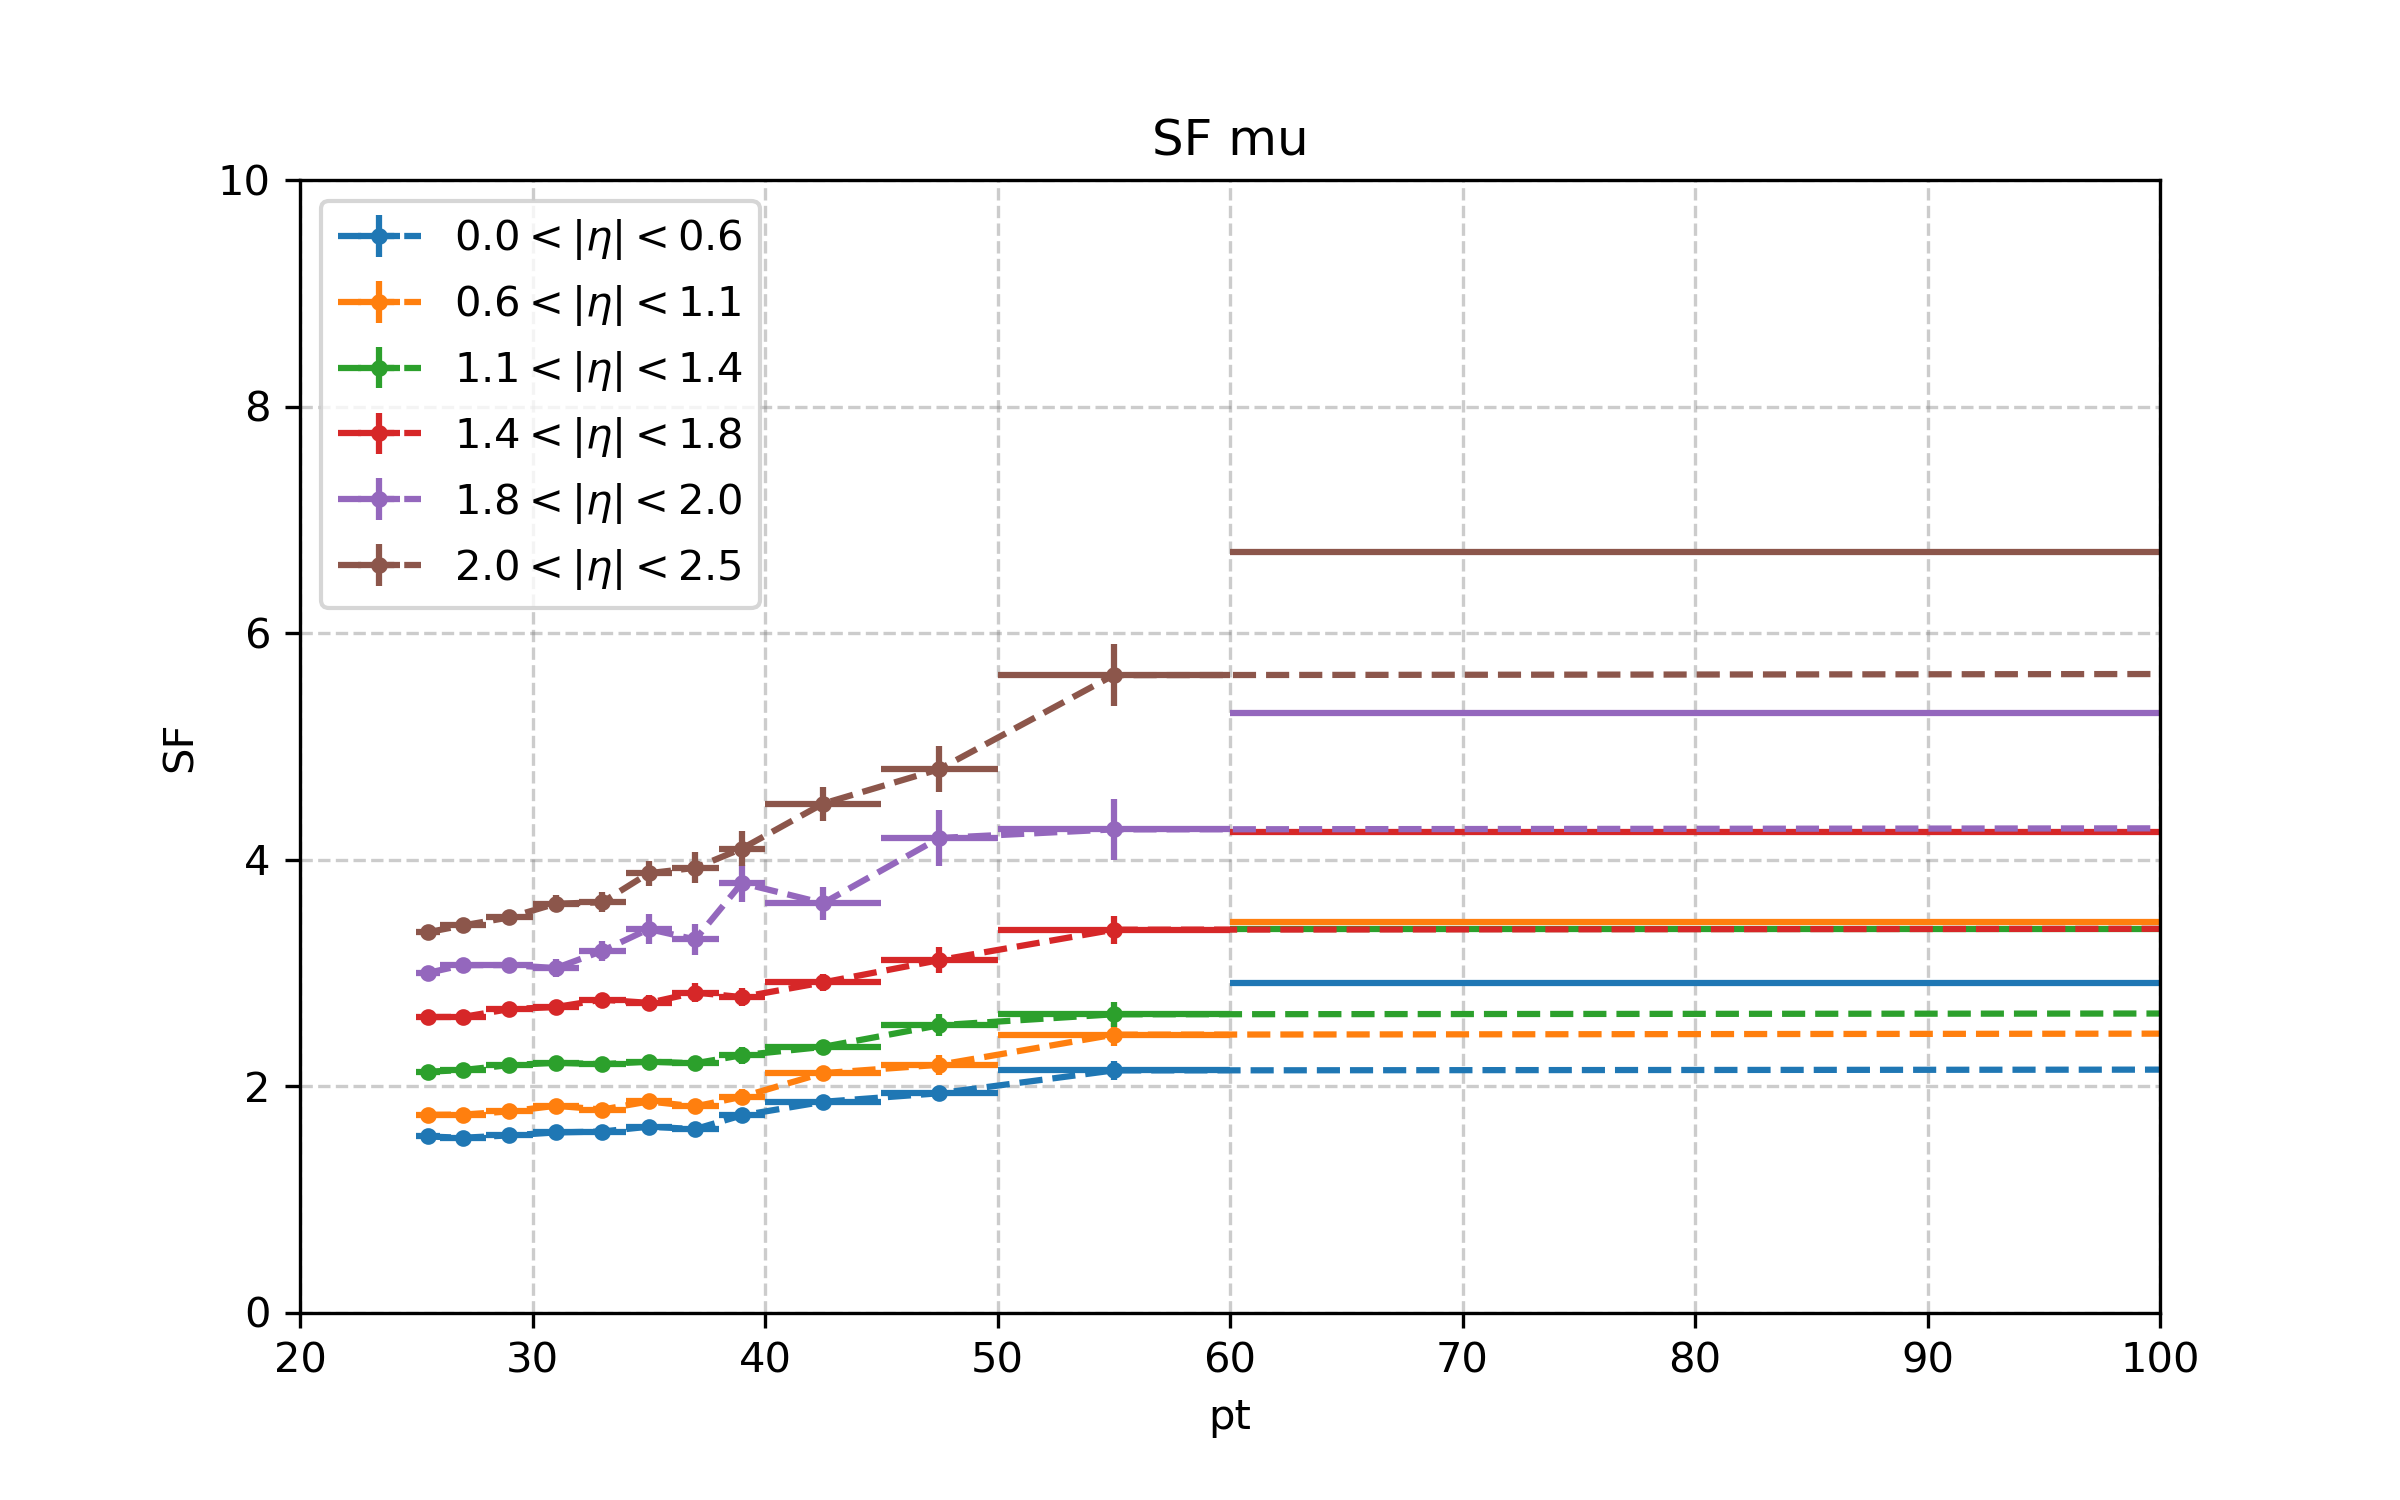
\includegraphics[width=0.49\textwidth]{chapters/Appendix/sectionQCD/figures/123j1b/SF_mu_1d.png}
    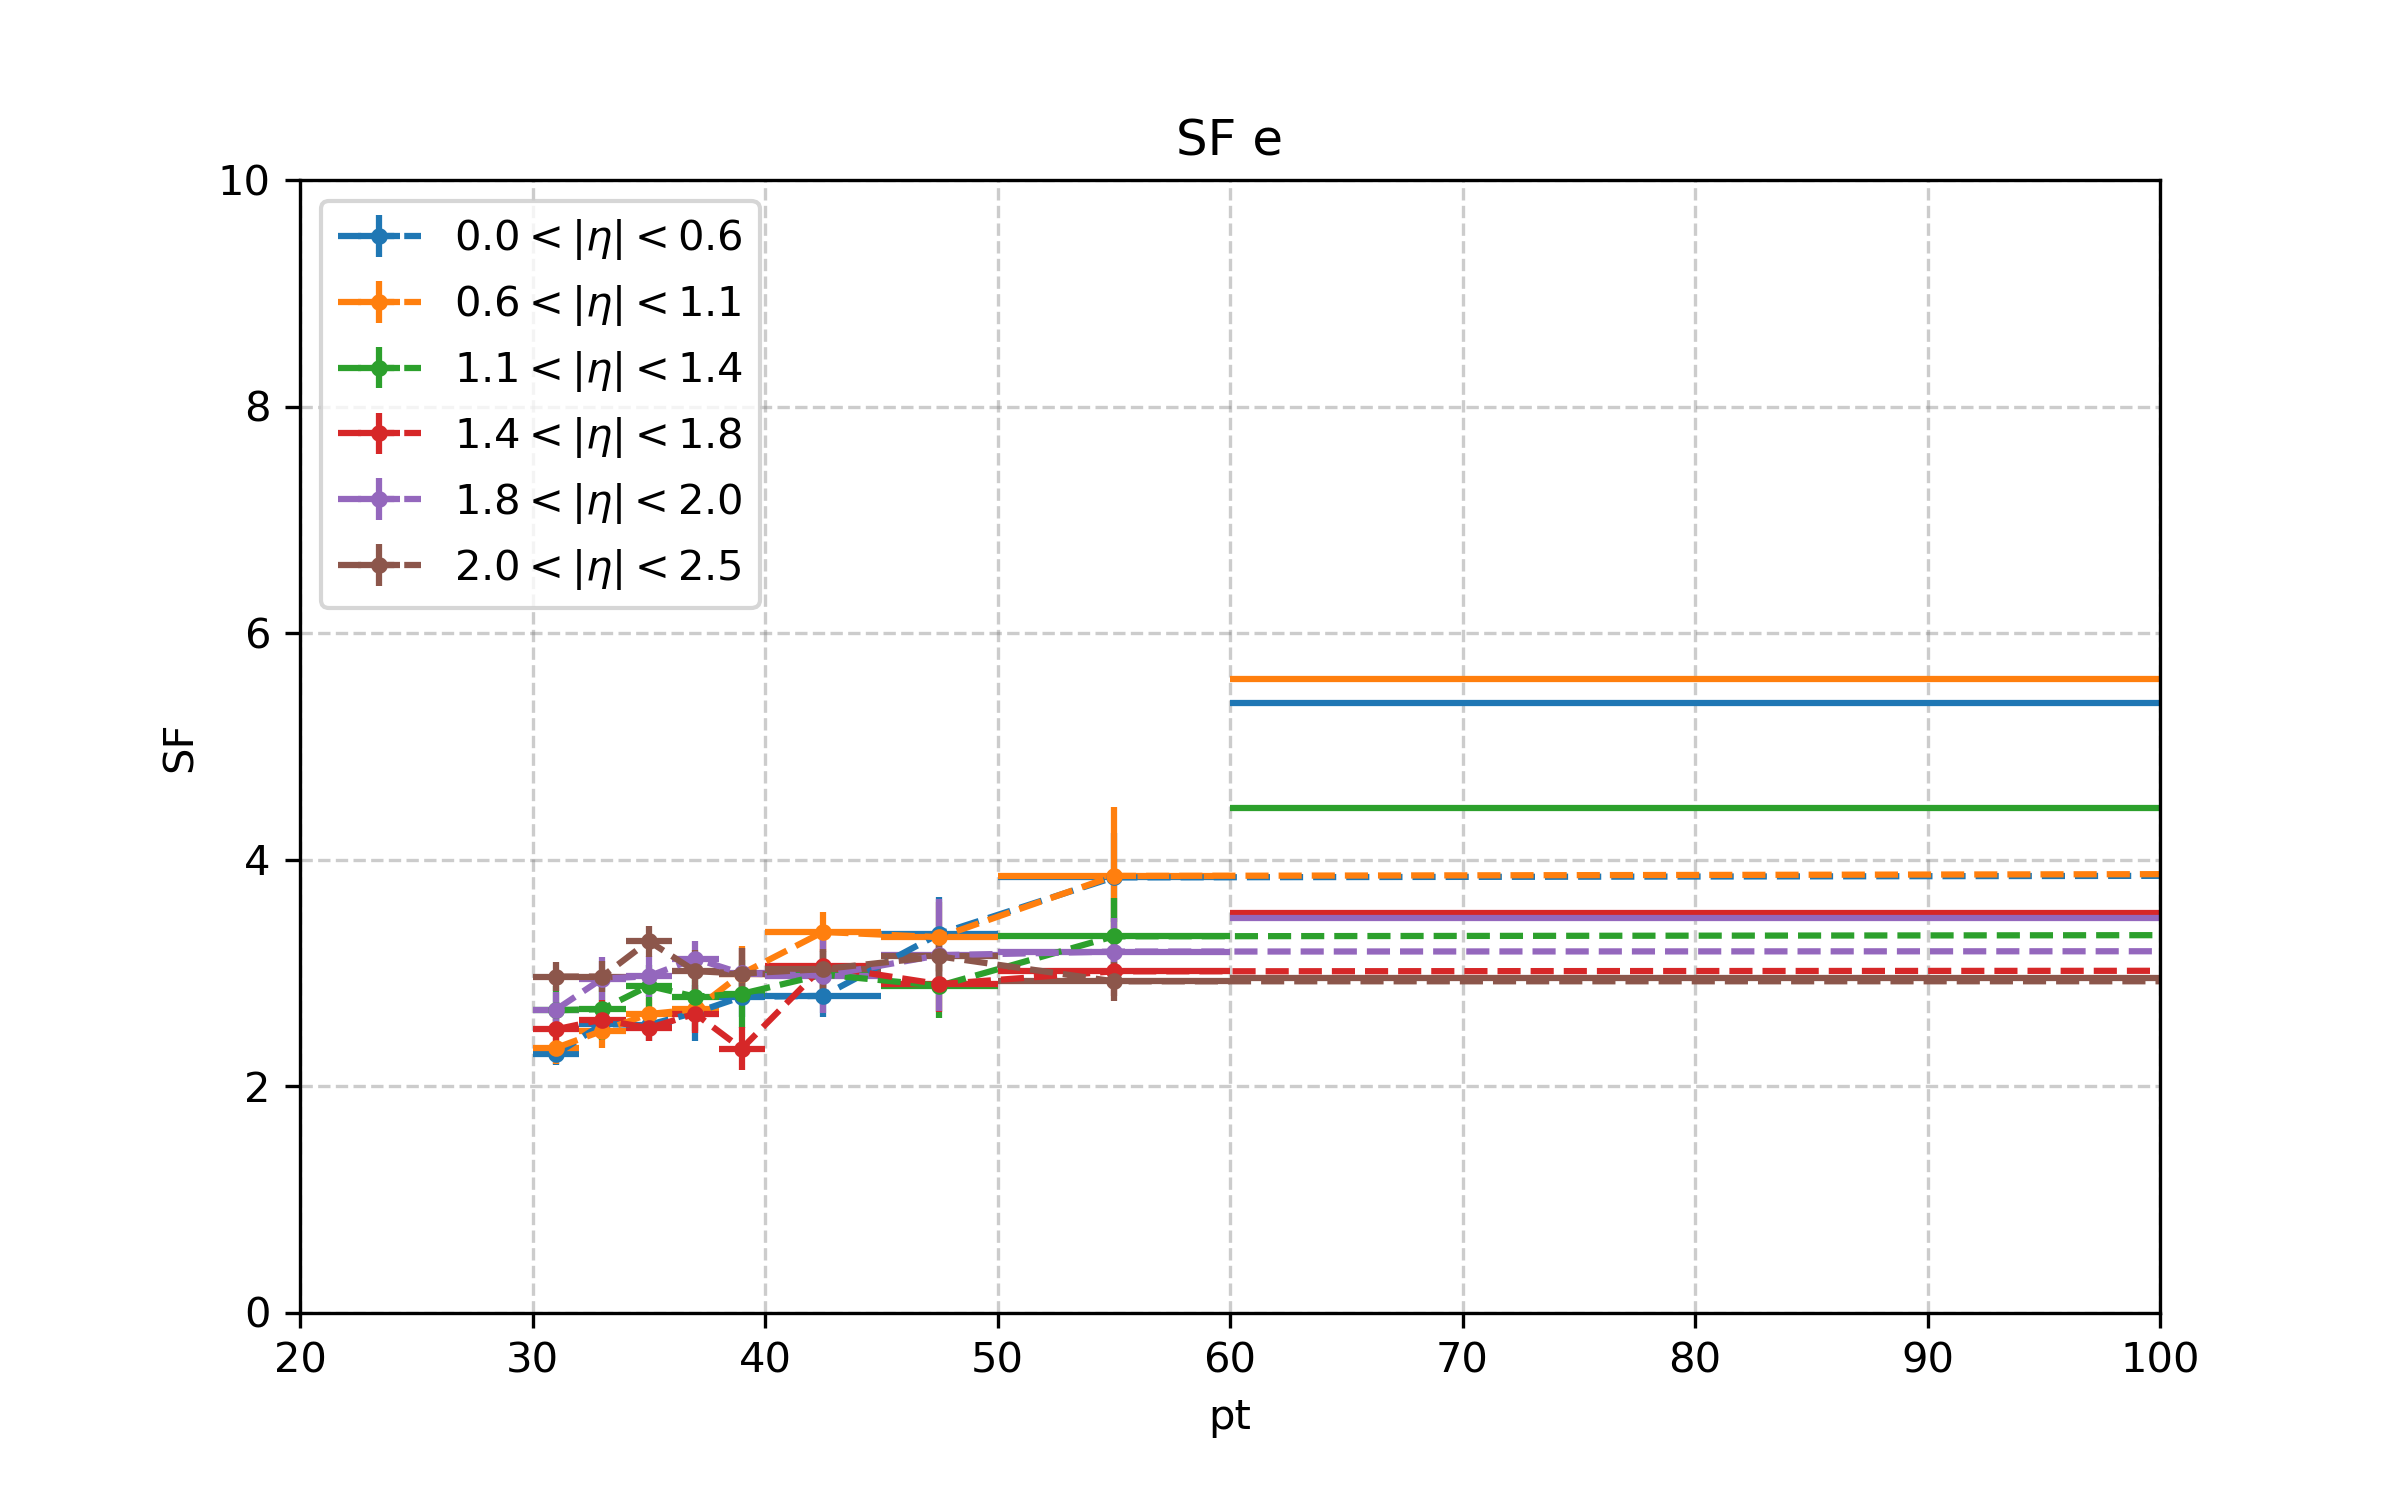
\includegraphics[width=0.49\textwidth]{chapters/Appendix/sectionQCD/figures/123j1b/SF_e_1d.png}
    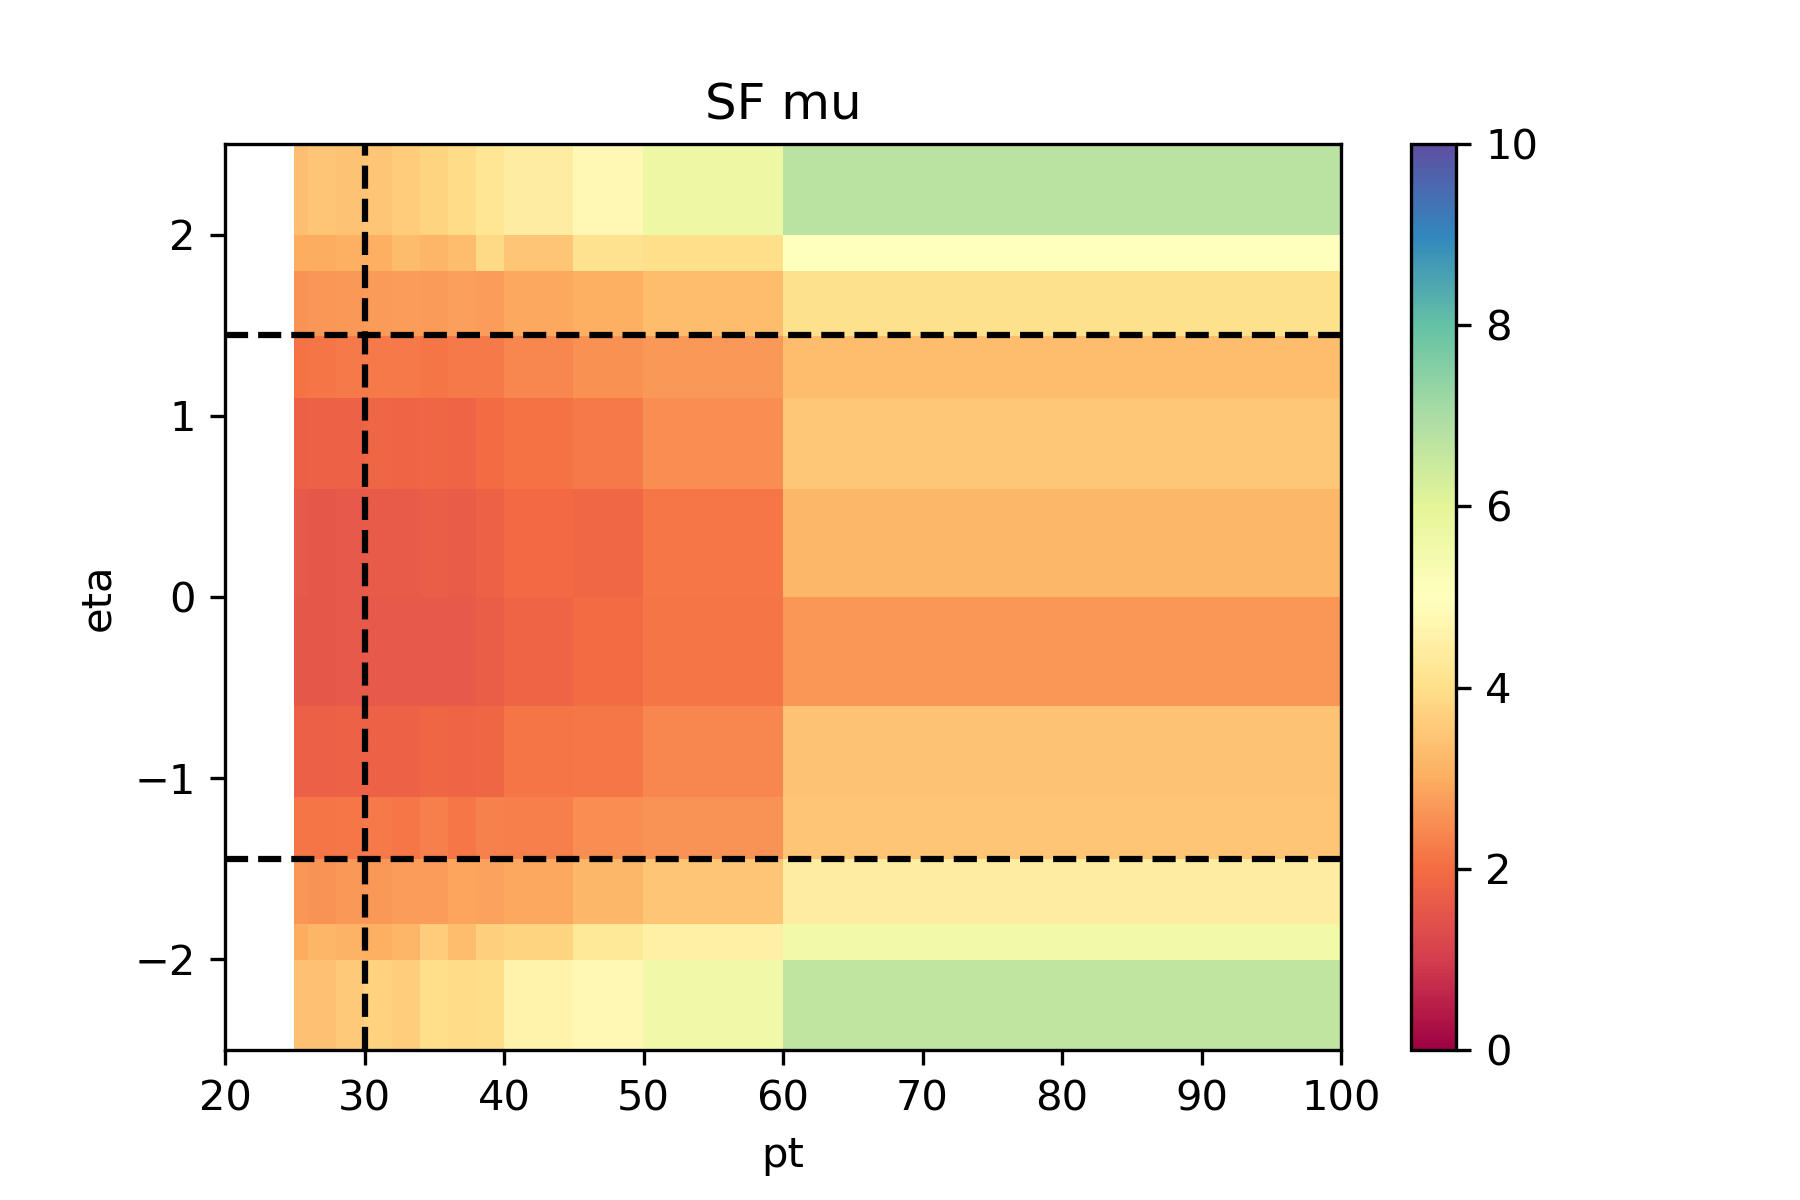
\includegraphics[width=0.49\textwidth]{chapters/Appendix/sectionQCD/figures/123j1b/SF_mu_2d.png}
    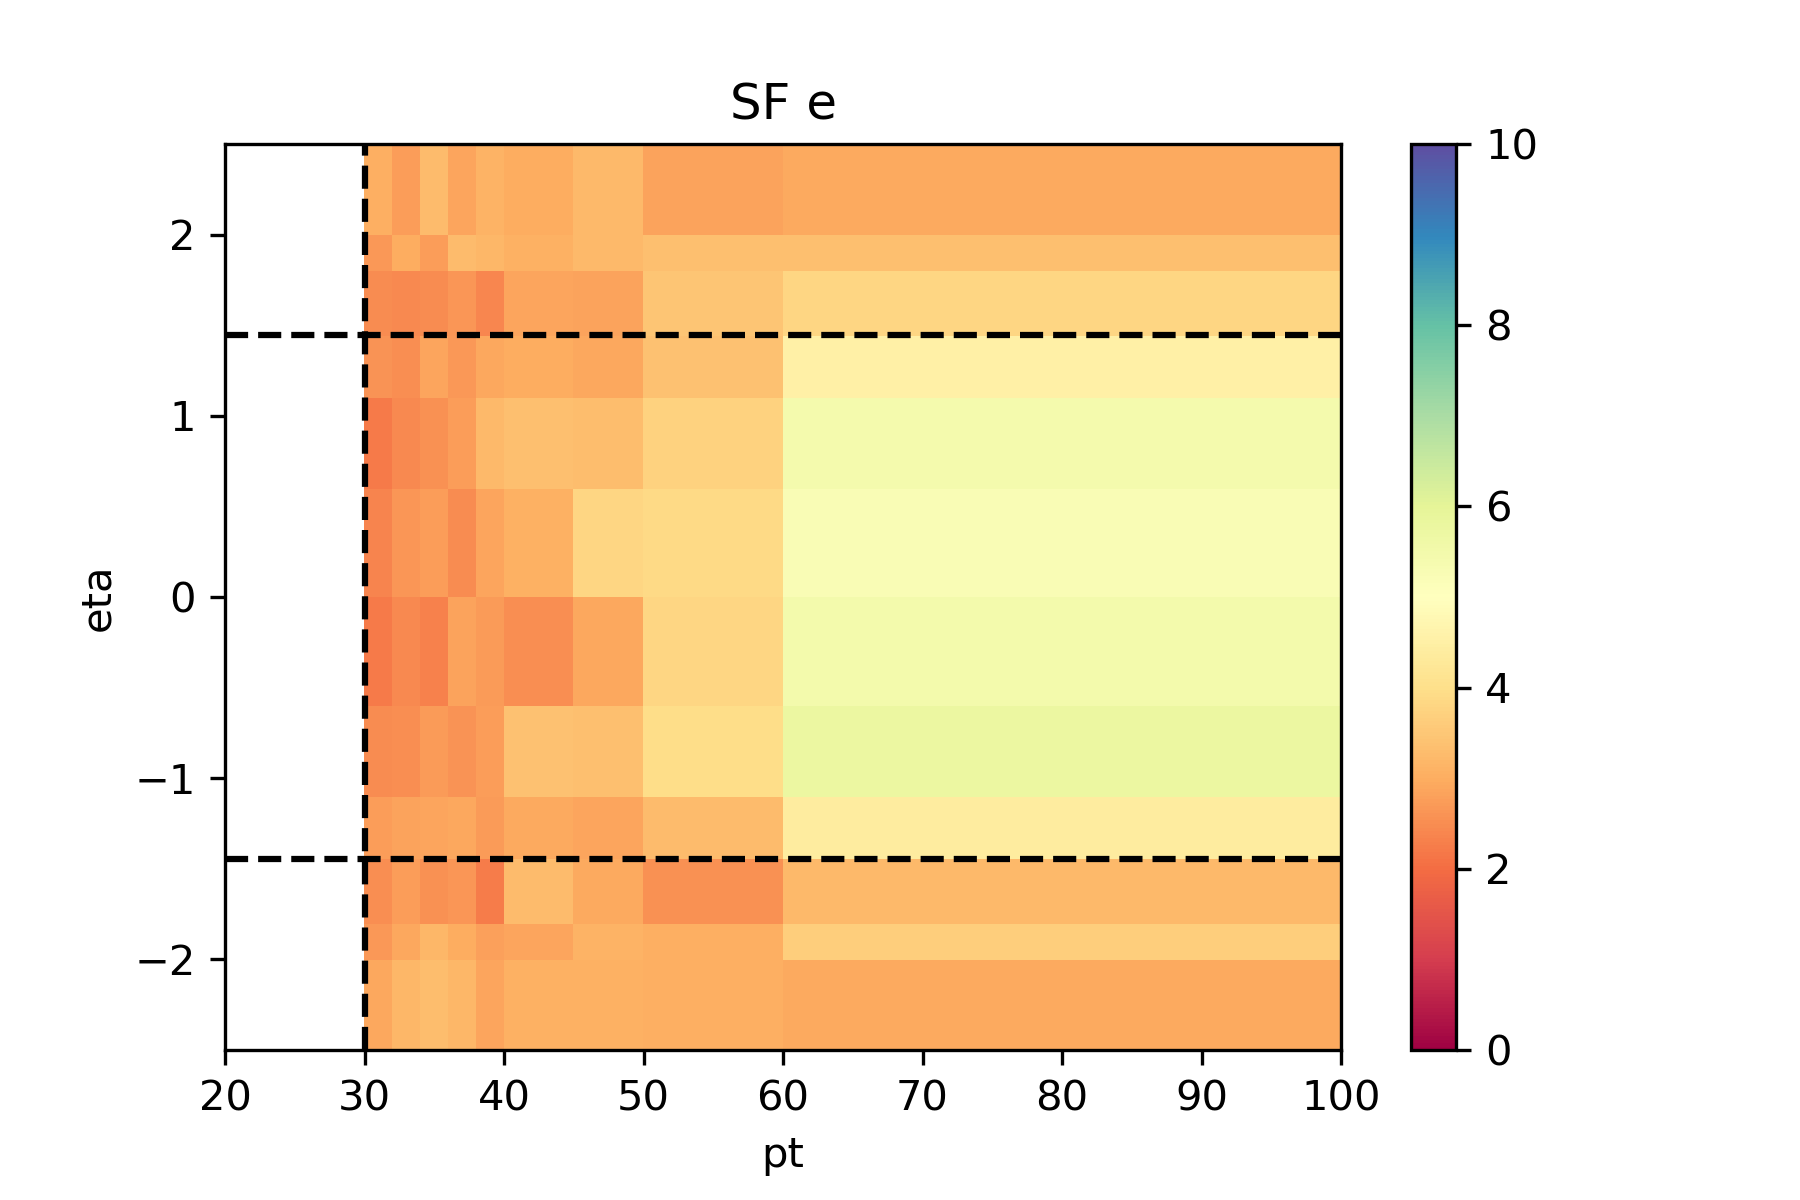
\includegraphics[width=0.49\textwidth]{chapters/Appendix/sectionQCD/figures/123j1b/SF_e_2d.png}

    \caption{iso-to-antiiso SF in the $\mu$+jet (left) and $e$+jet (right) channel 
    with $1\leq n_j <4, n_b\geq1$ side-band region.}
    \label{fig:appendix:123j1b_sf}
\end{figure}



\begin{figure}
    \centering
    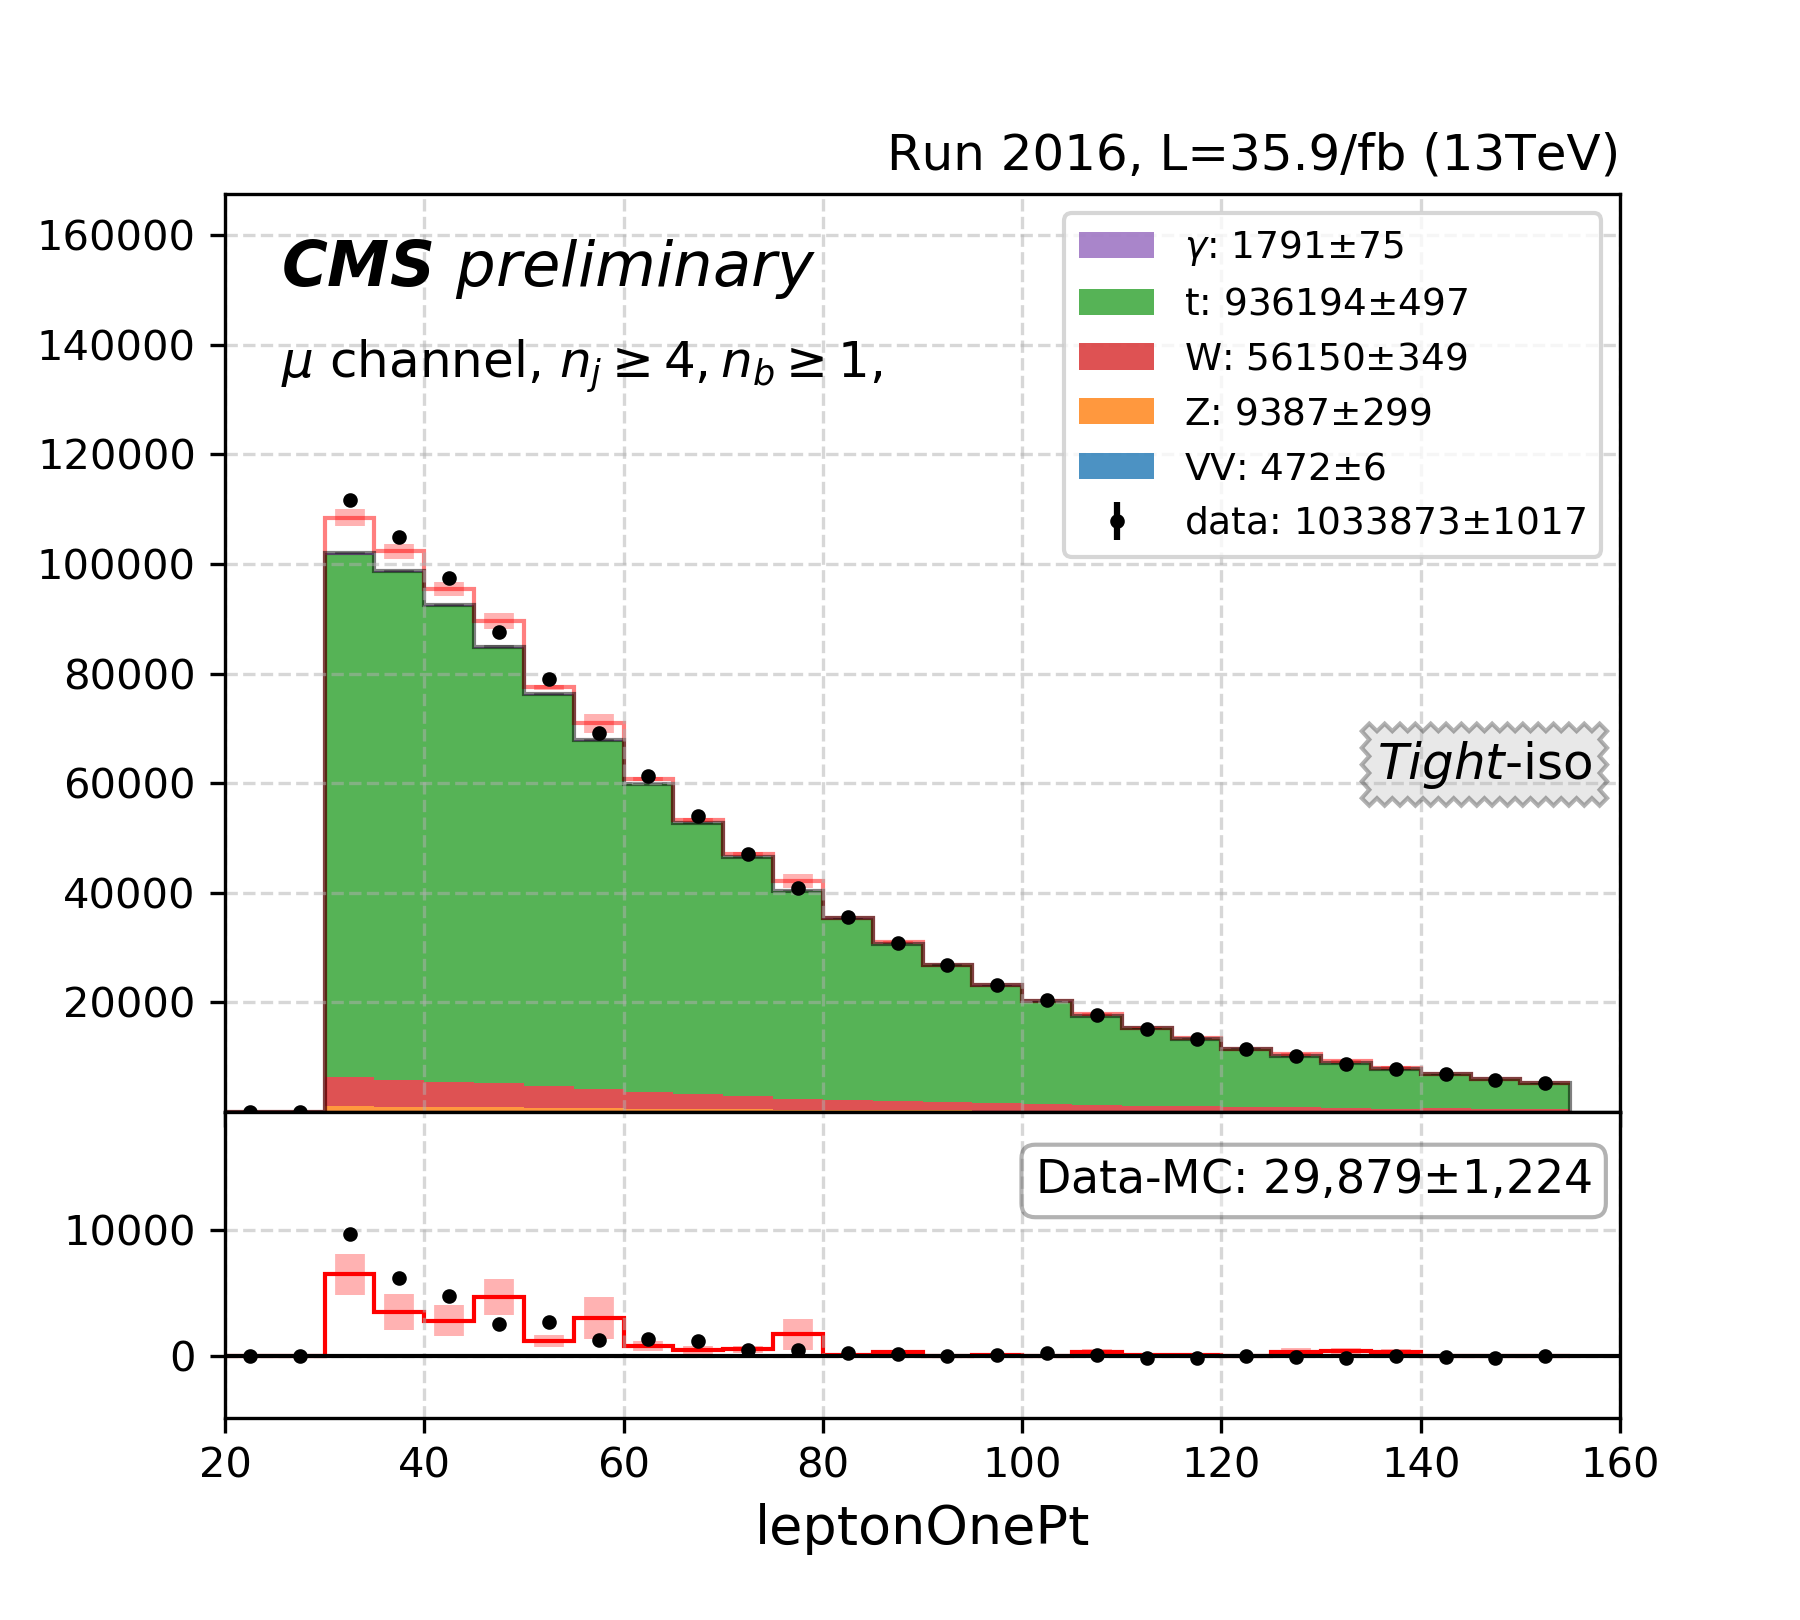
\includegraphics[width=0.24\textwidth]{chapters/Appendix/sectionQCD/figures/4j1b/mu_leptonOnePt_True_mcqcd.png}
    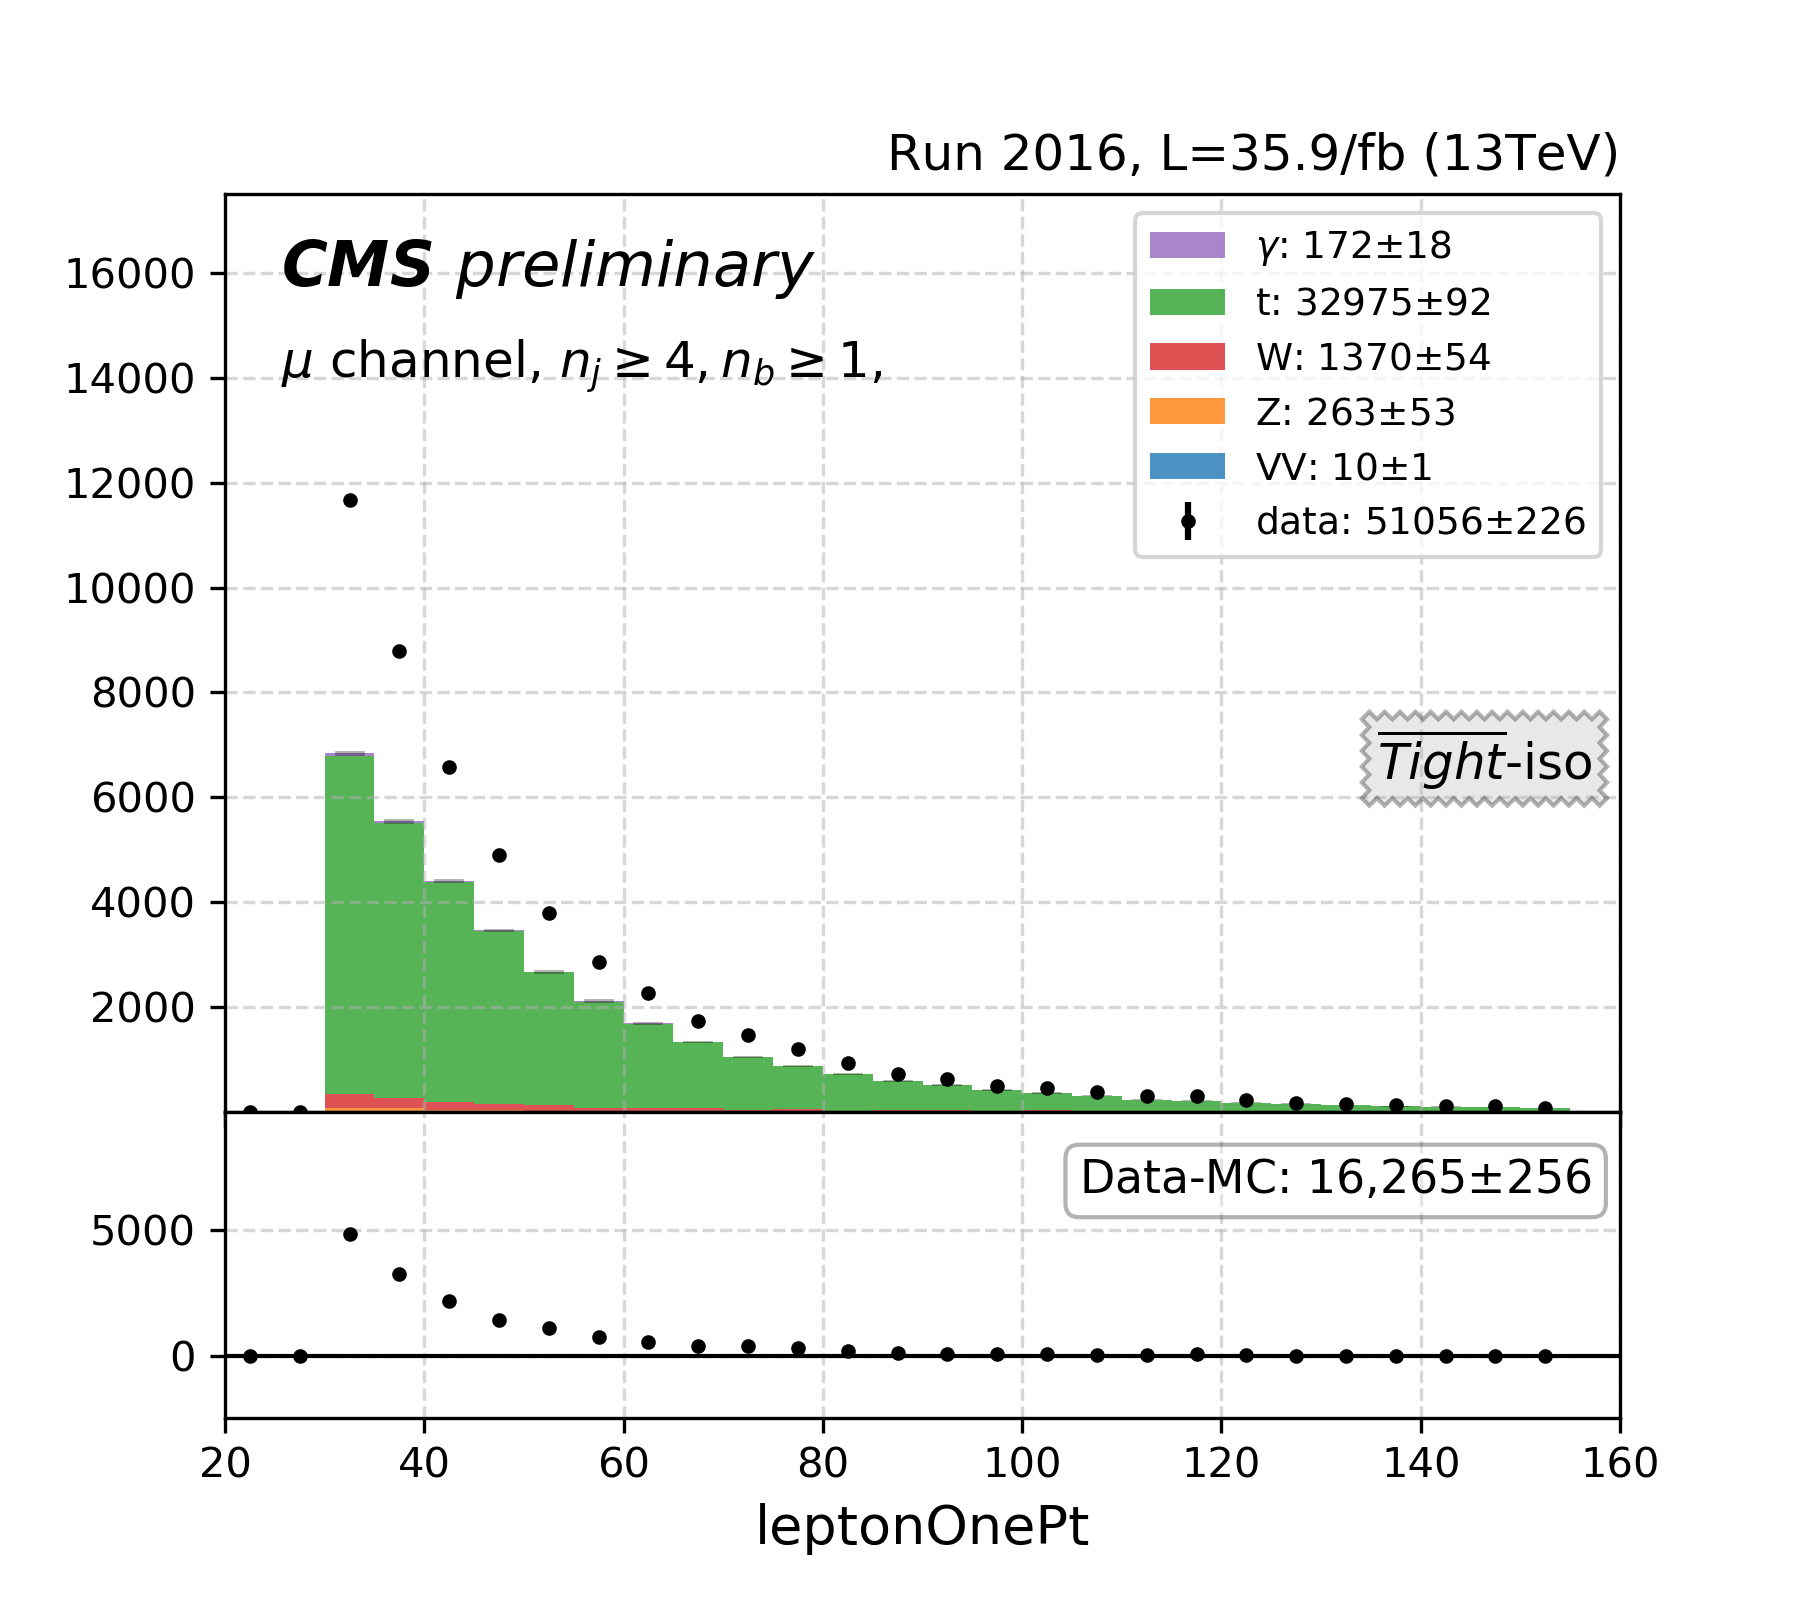
\includegraphics[width=0.24\textwidth]{chapters/Appendix/sectionQCD/figures/4j1b/mu_leptonOnePt_False.png}
    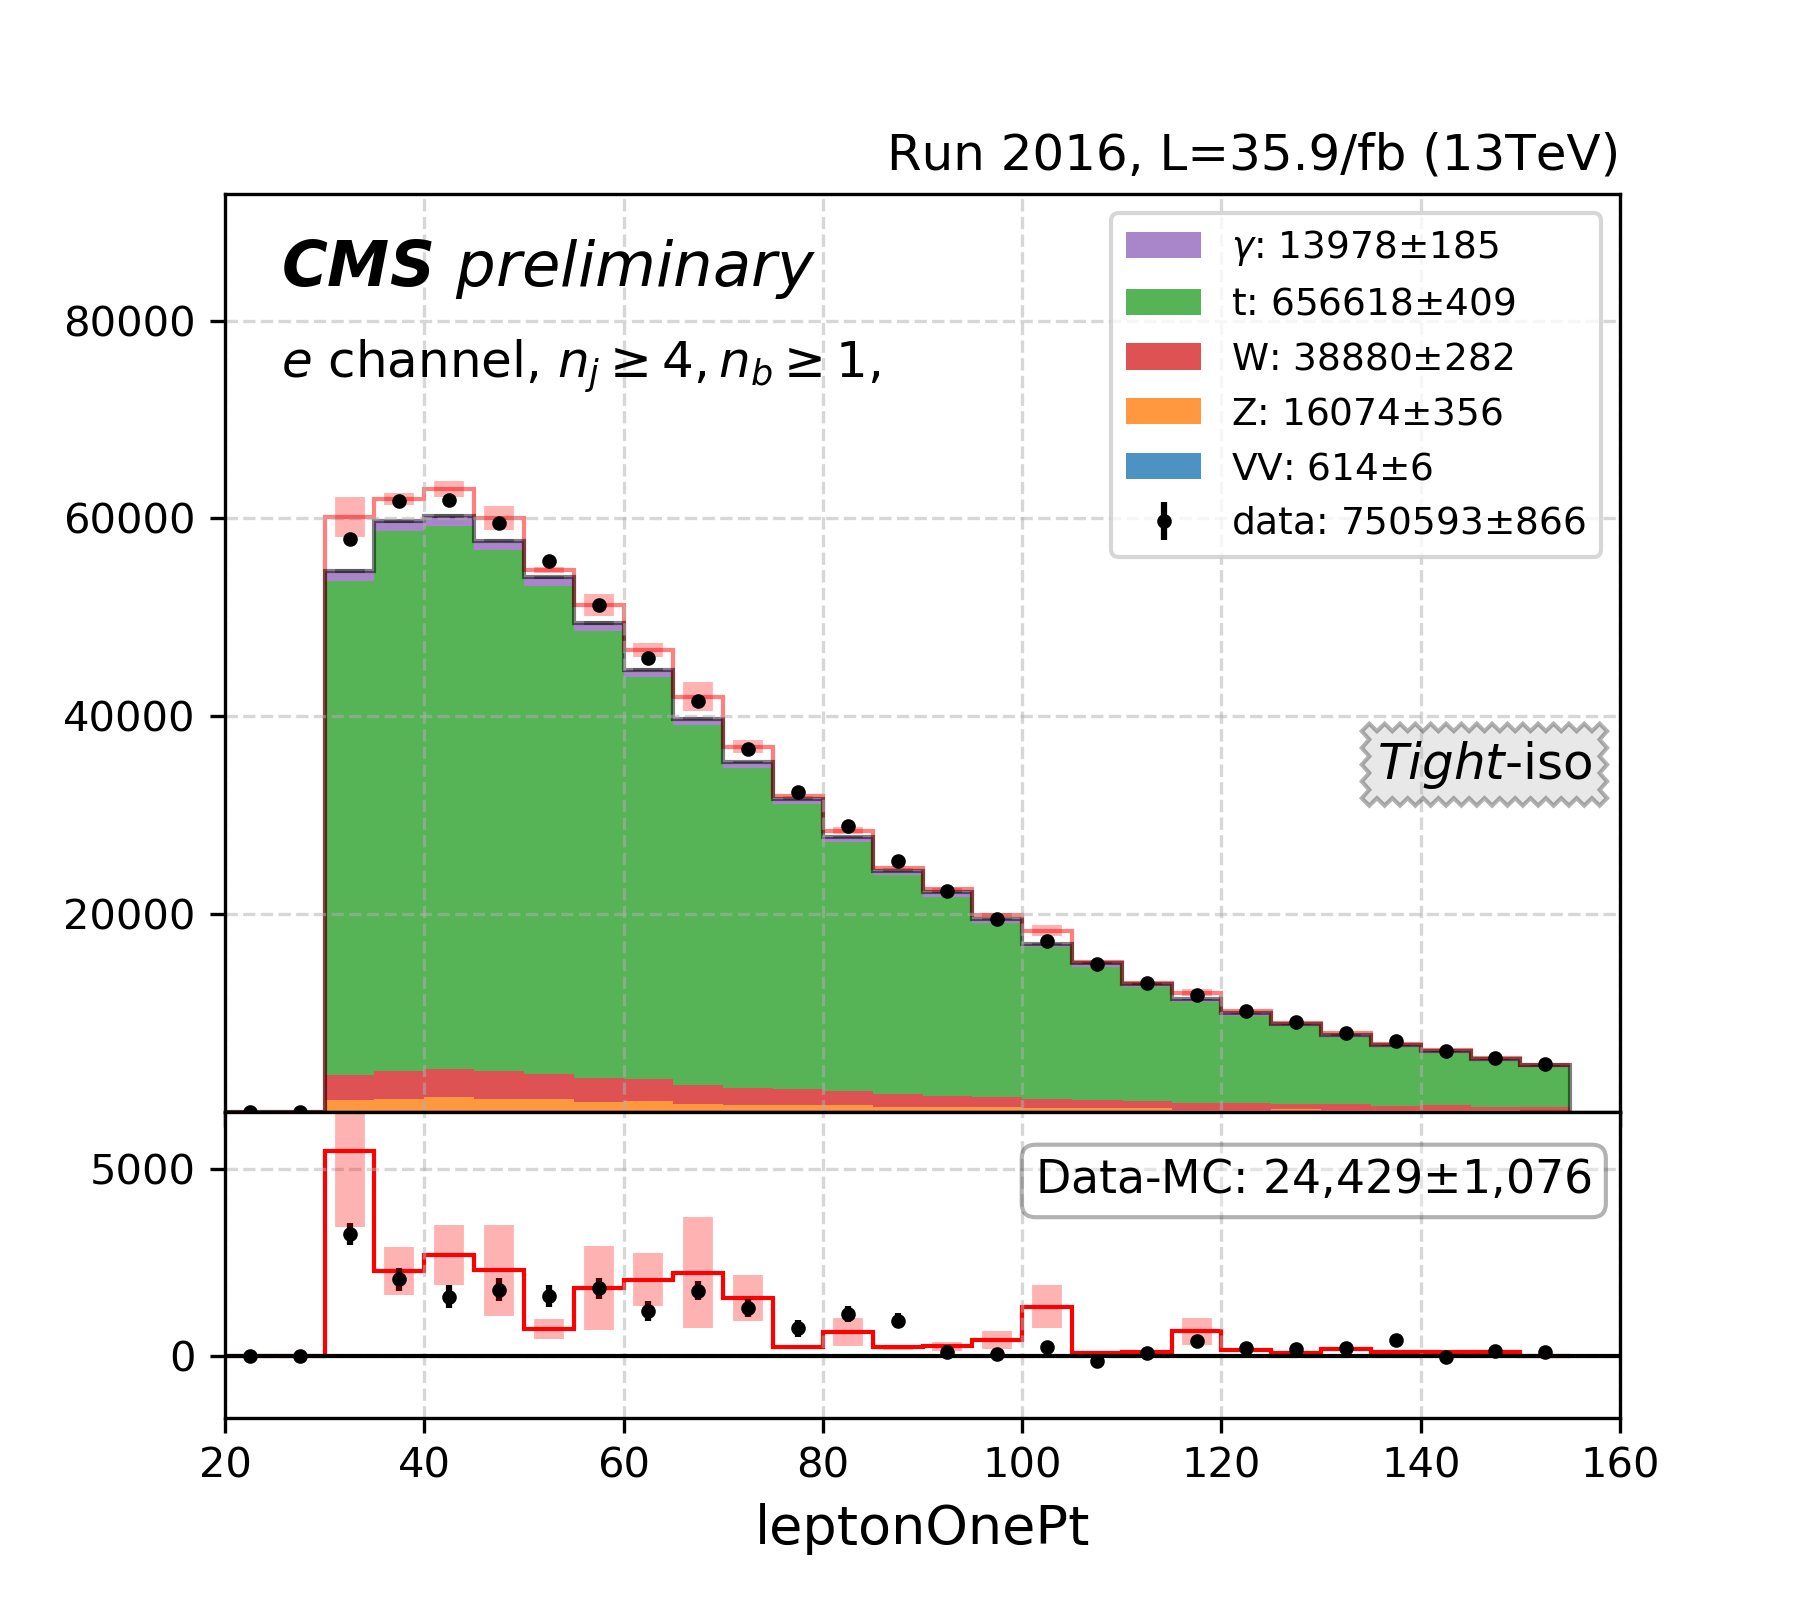
\includegraphics[width=0.24\textwidth]{chapters/Appendix/sectionQCD/figures/4j1b/e_leptonOnePt_True_mcqcd.png}
    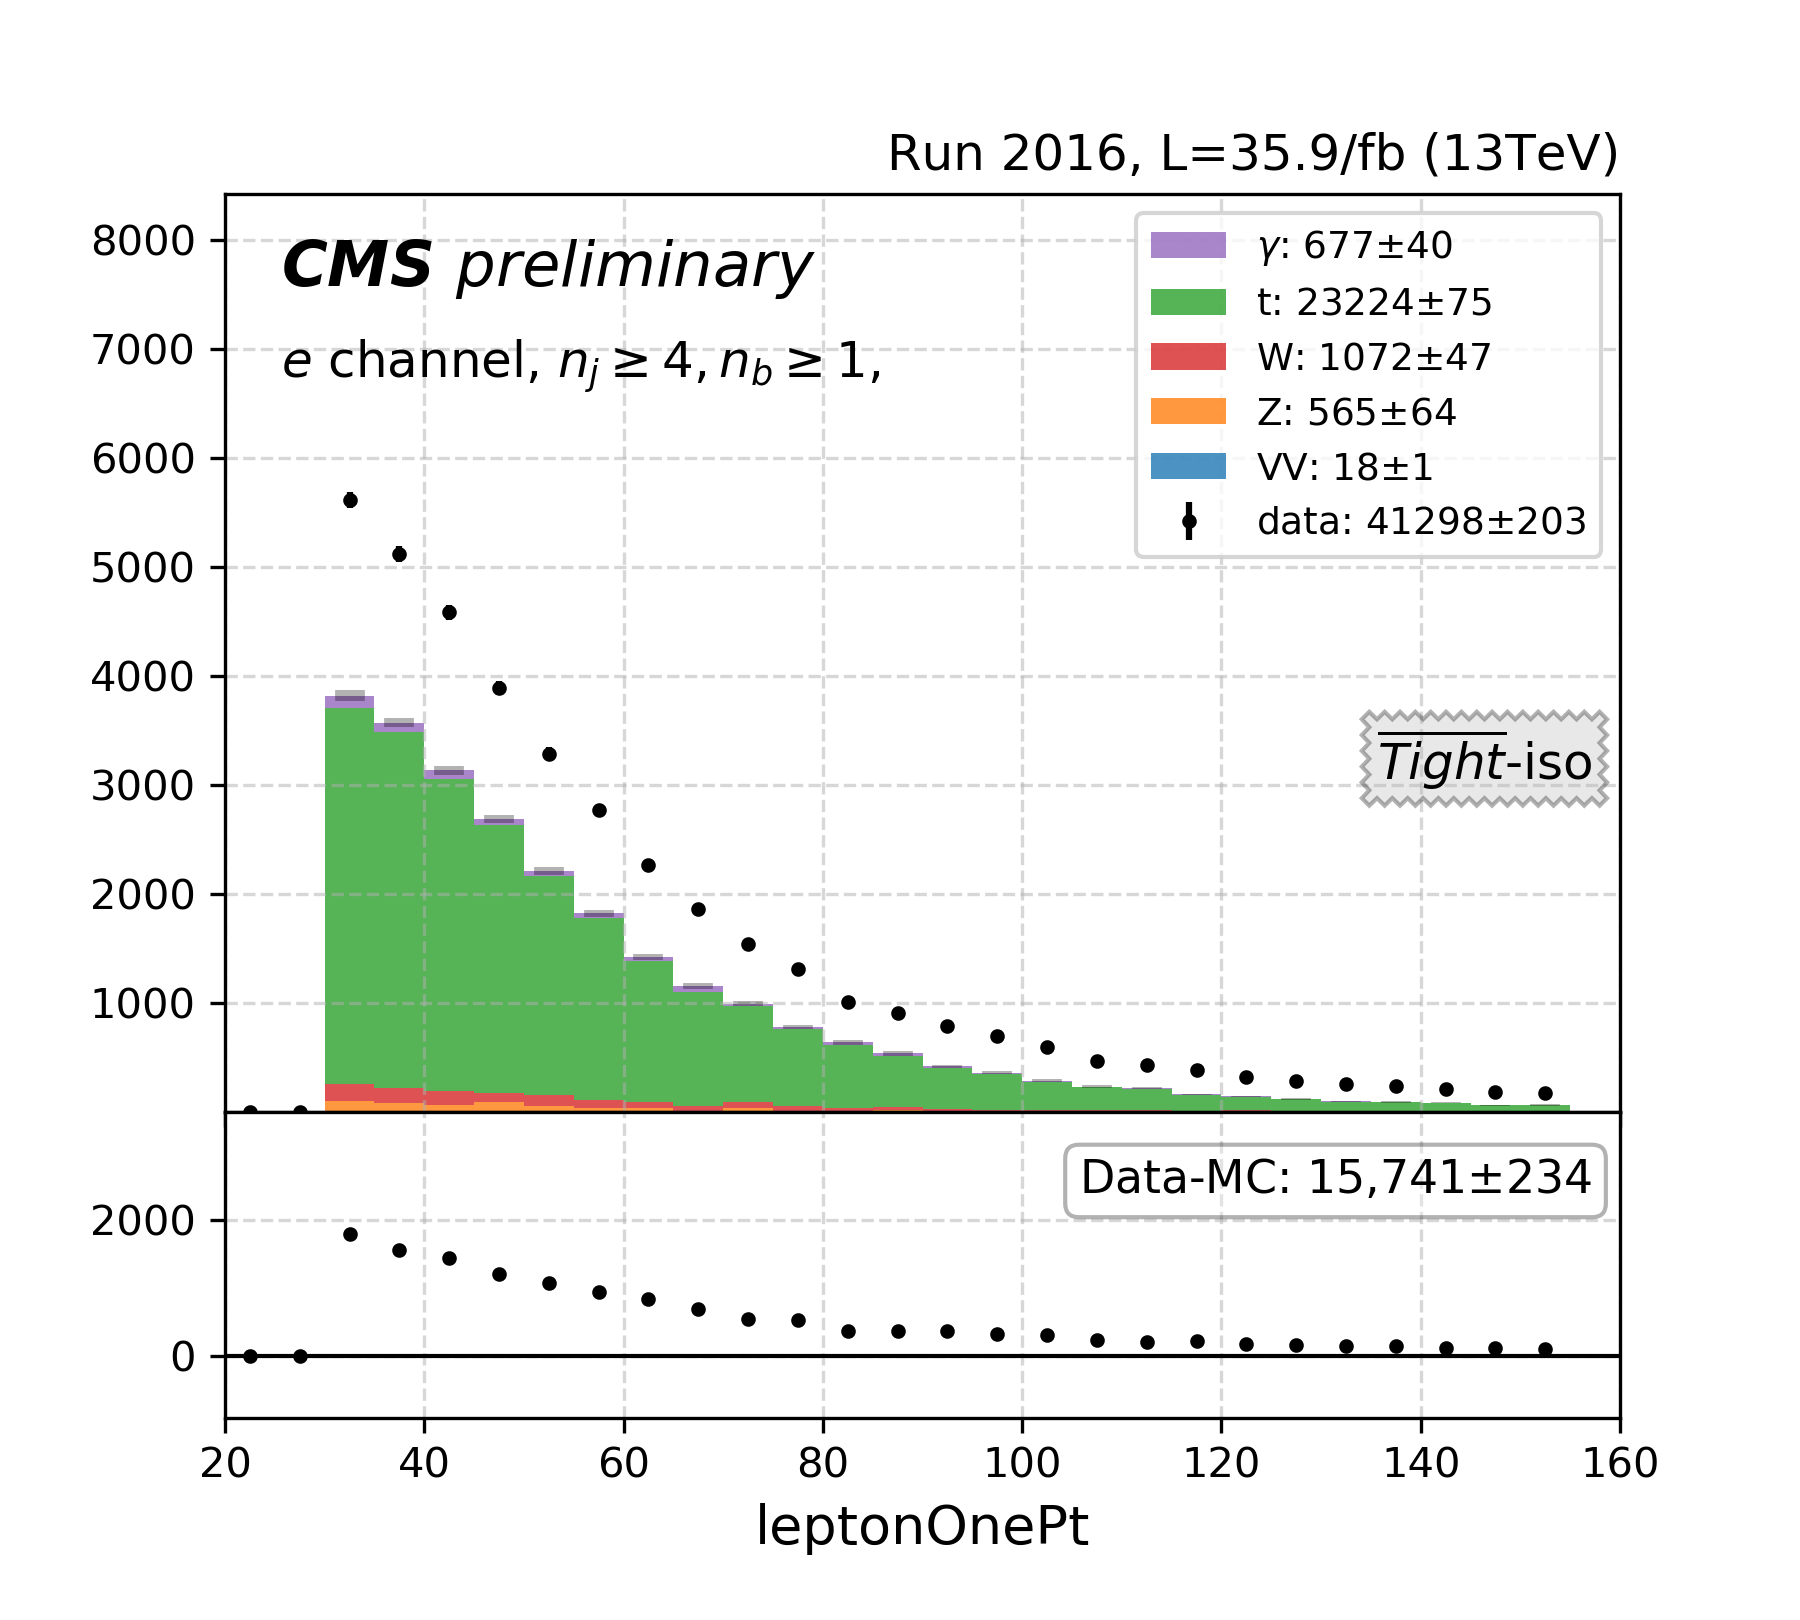
\includegraphics[width=0.24\textwidth]{chapters/Appendix/sectionQCD/figures/4j1b/e_leptonOnePt_False.png}
    
    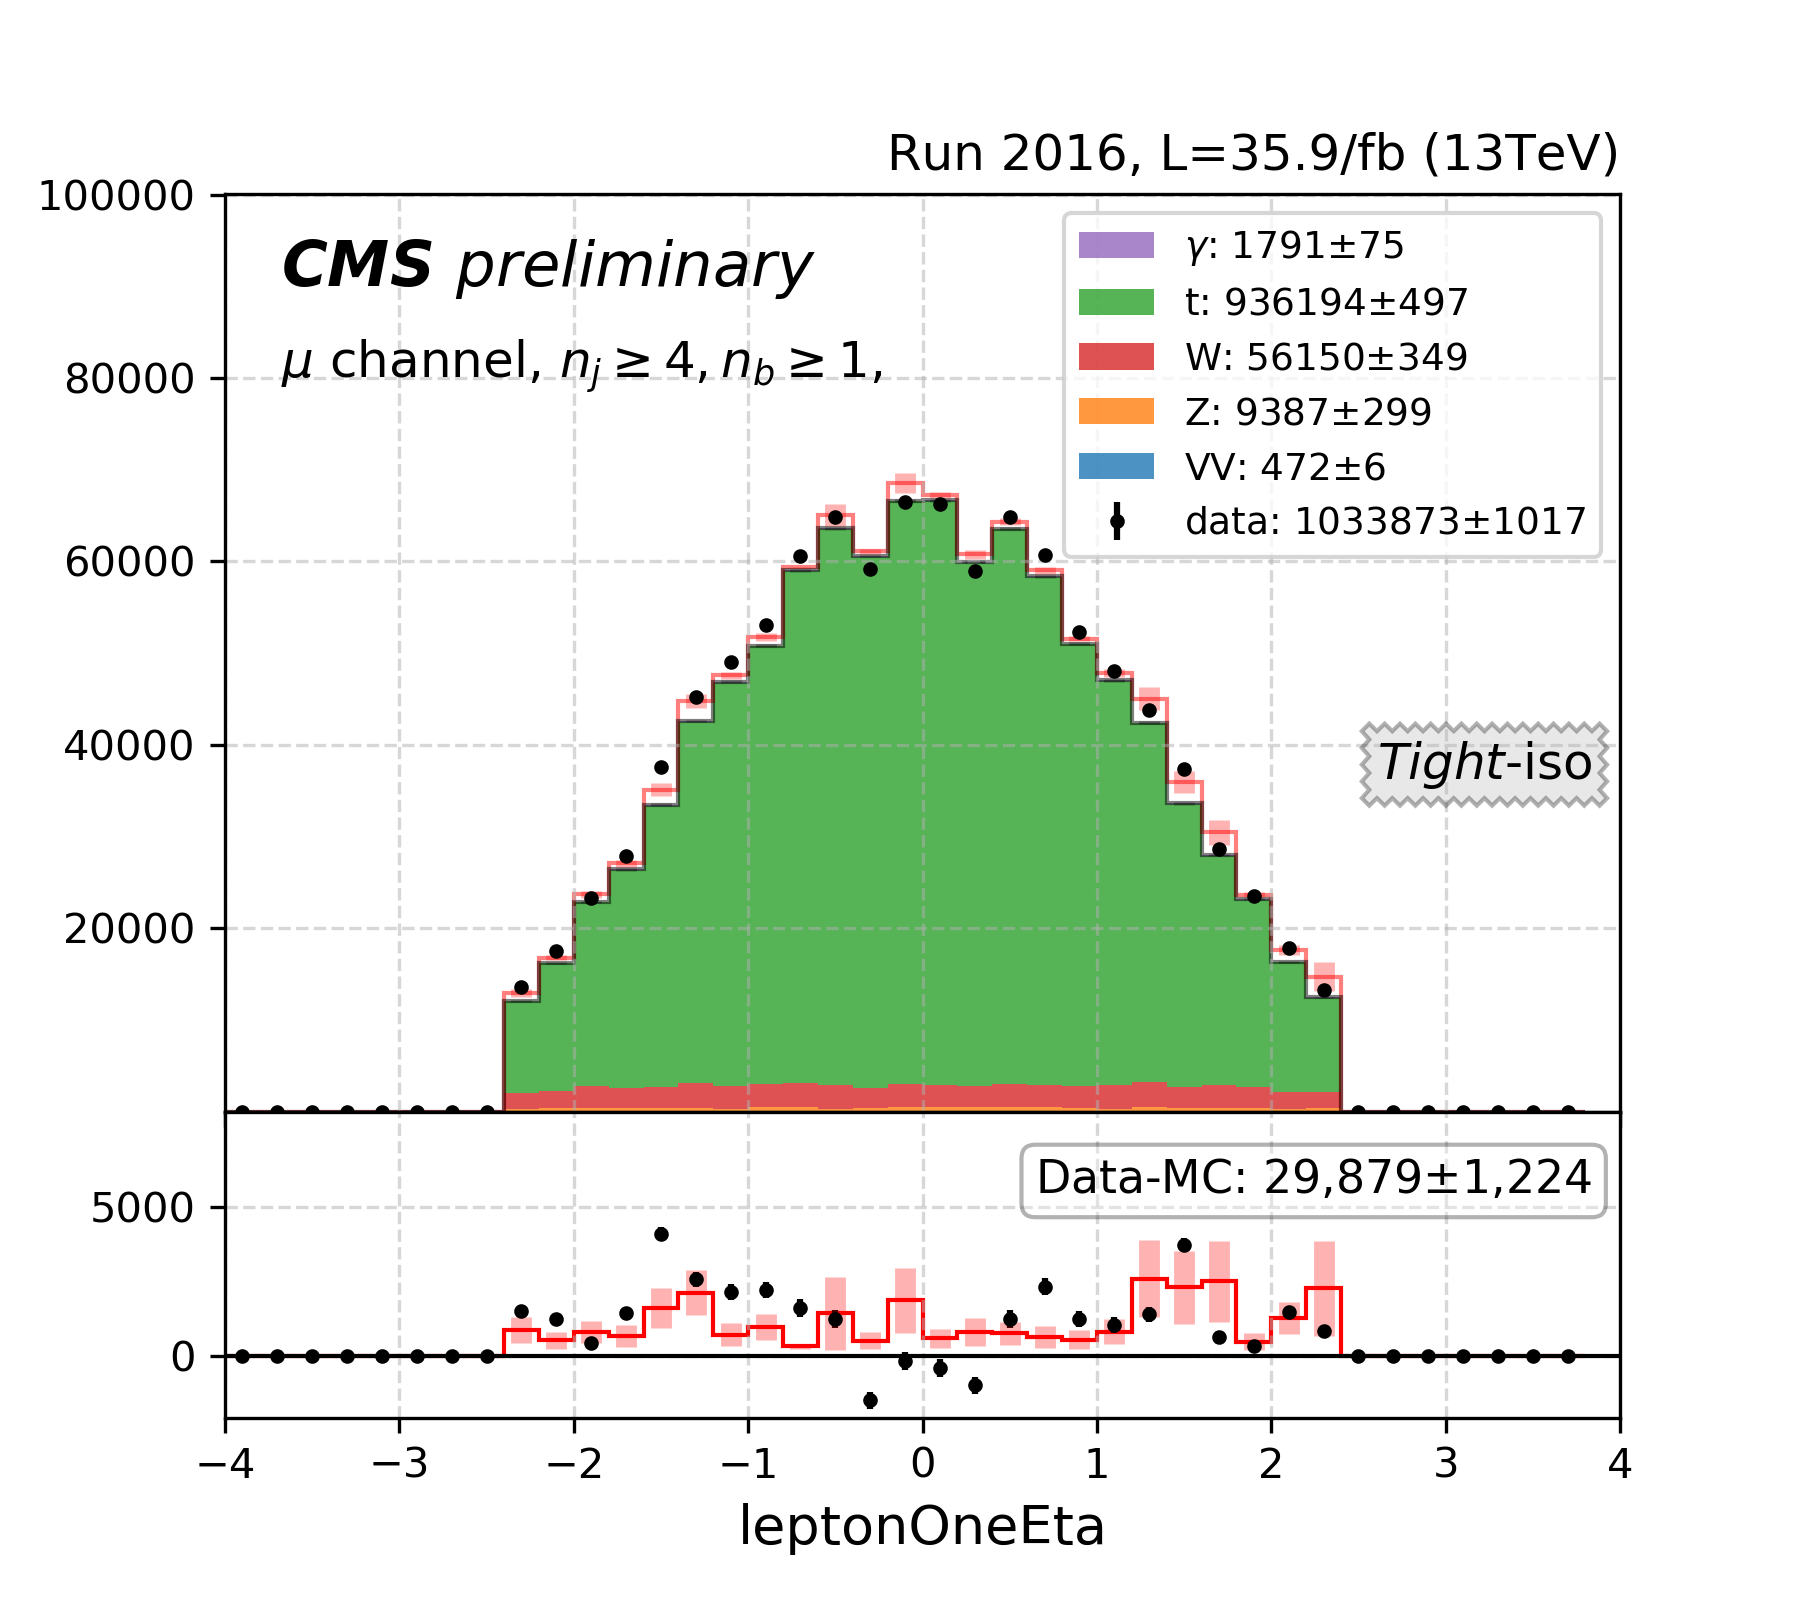
\includegraphics[width=0.24\textwidth]{chapters/Appendix/sectionQCD/figures/4j1b/mu_leptonOneEta_True_mcqcd.png}
    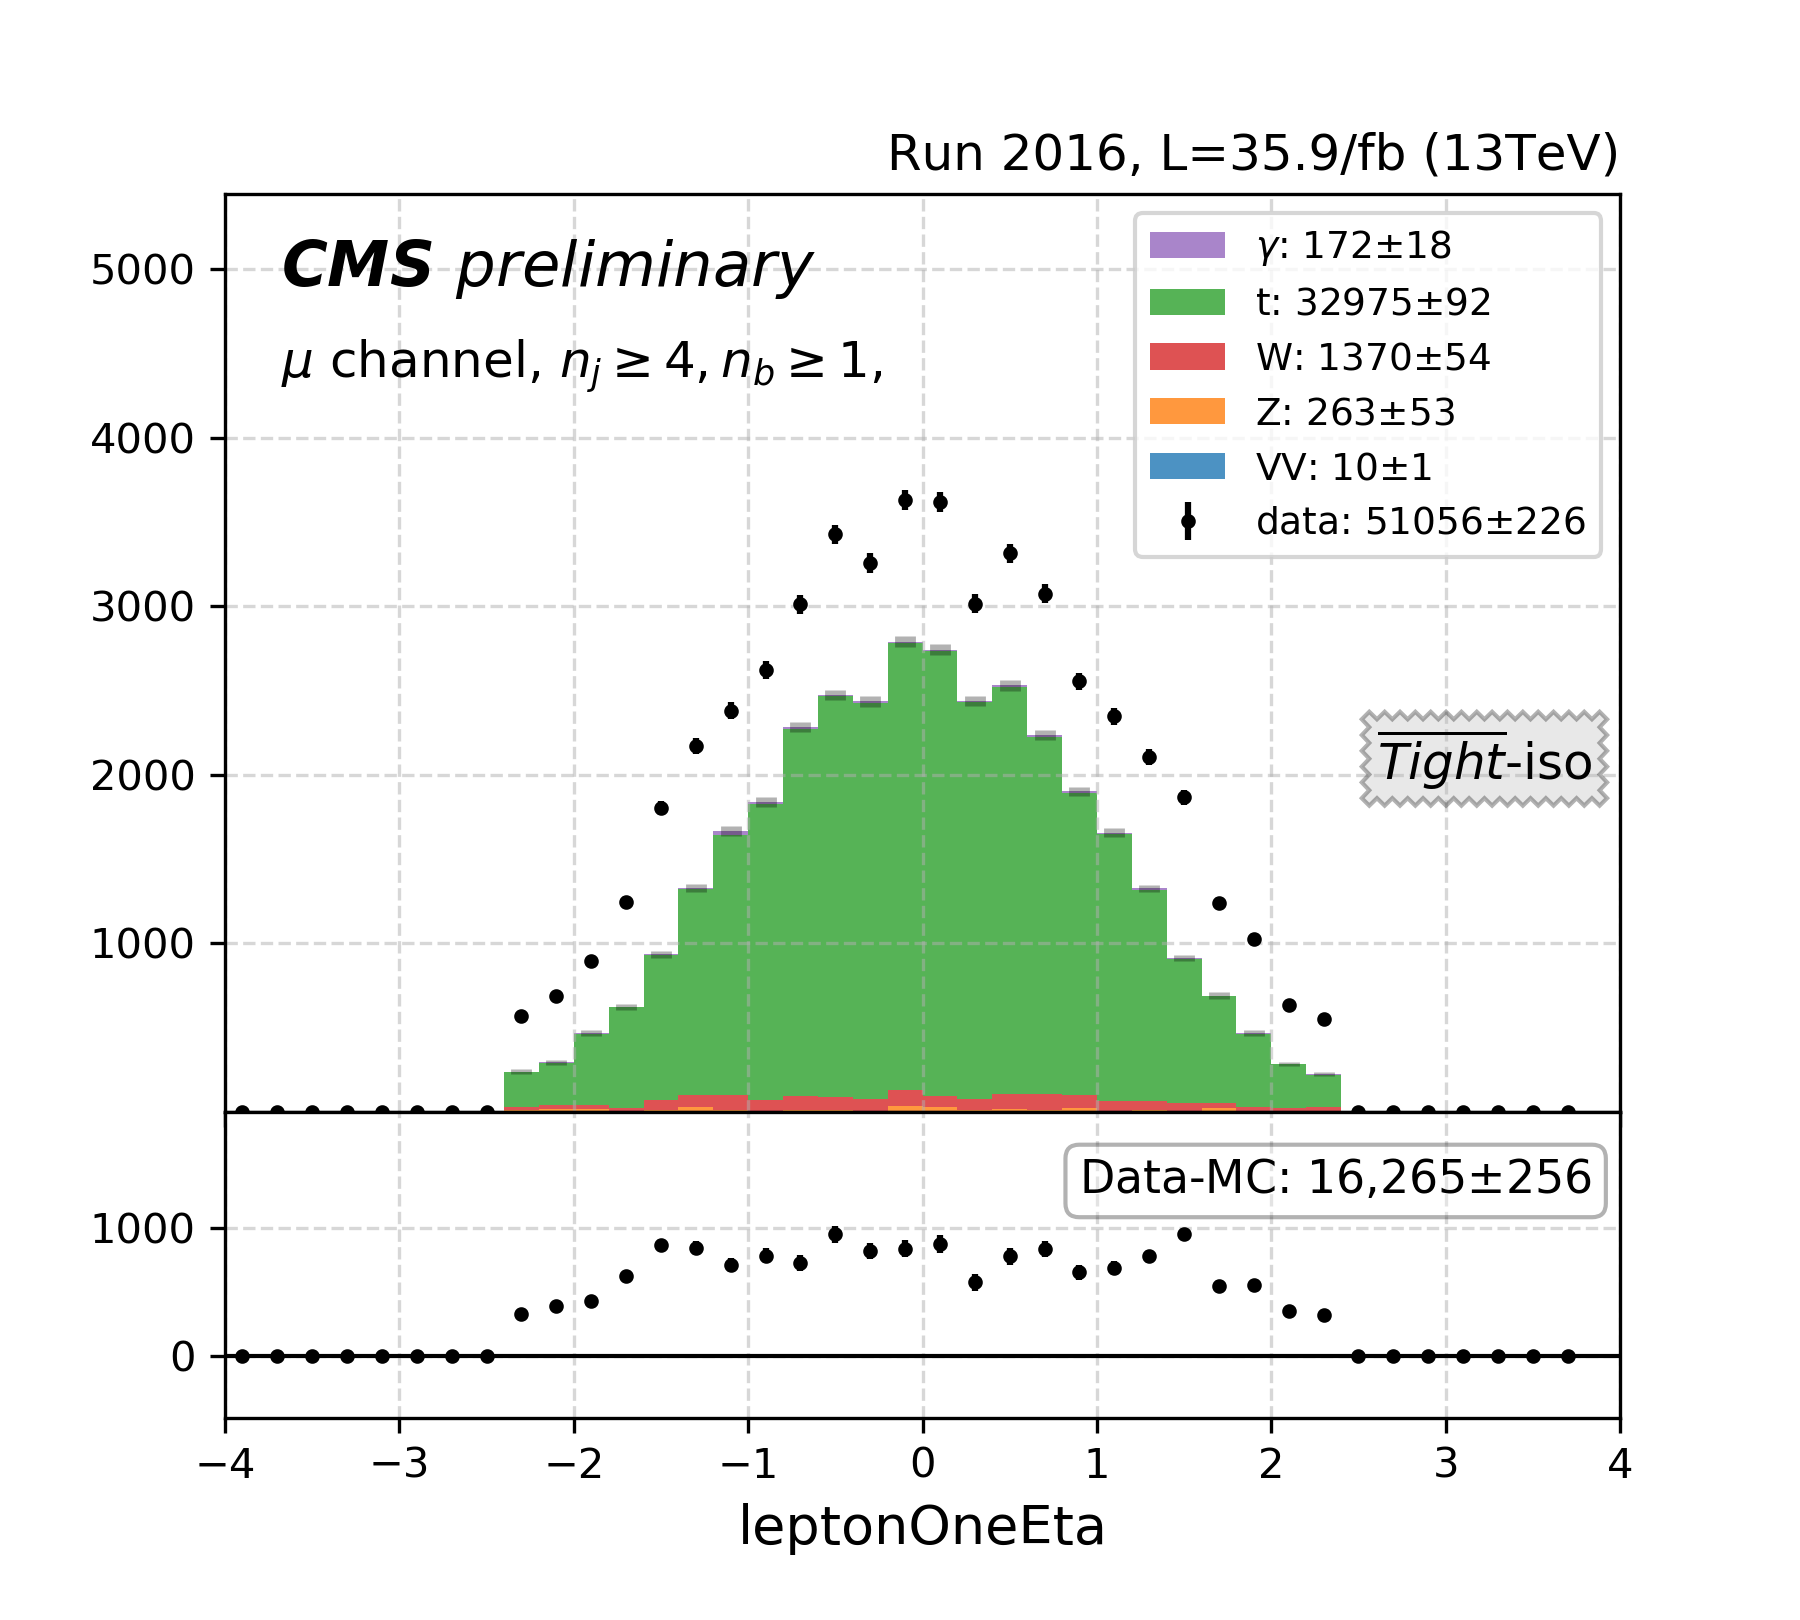
\includegraphics[width=0.24\textwidth]{chapters/Appendix/sectionQCD/figures/4j1b/mu_leptonOneEta_False.png}
    \includegraphics[width=0.24\textwidth]{chapters/Appendix/sectionQCD/figures/4j1b/e_leptonOneEta_True_mcqcd.png}
    \includegraphics[width=0.24\textwidth]{chapters/Appendix/sectionQCD/figures/4j1b/e_leptonOneEta_False.png}
    
    \includegraphics[width=0.24\textwidth]{chapters/Appendix/sectionQCD/figures/4j1b/mu_nJets_True_mcqcd.png}
    \includegraphics[width=0.24\textwidth]{chapters/Appendix/sectionQCD/figures/4j1b/mu_nJets_False.png}
    \includegraphics[width=0.24\textwidth]{chapters/Appendix/sectionQCD/figures/4j1b/e_nJets_True_mcqcd.png}
    \includegraphics[width=0.24\textwidth]{chapters/Appendix/sectionQCD/figures/4j1b/e_nJets_False.png}
    
    \includegraphics[width=0.24\textwidth]{chapters/Appendix/sectionQCD/figures/4j1b/mu_nBJets_True_mcqcd.png}
    \includegraphics[width=0.24\textwidth]{chapters/Appendix/sectionQCD/figures/4j1b/mu_nBJets_False.png}
    \includegraphics[width=0.24\textwidth]{chapters/Appendix/sectionQCD/figures/4j1b/e_nBJets_True_mcqcd.png}
    \includegraphics[width=0.24\textwidth]{chapters/Appendix/sectionQCD/figures/4j1b/e_nBJets_False.png}
    

    \caption{The iso and anti-iso region of $\mu$+jet (left two columns) and $e$+jet (right two columns) channel 
    with $n_j\geq4,n_b\geq1$, the signal region.}
    \label{fig:appendix:4j1b}
\end{figure}
\FloatBarrier